% !TeX spellcheck = pt_BR

\chapter{Dinâmica - Descrição Escalar}

\section*{O que é}

Vamos agora dar início a uma nova formulação da dinâmica -- do estudo das causas do movimento dos corpos. Contudo, construiremos agora uma linguagem 100\% escalar: trabalho e energia, os conceitos chave que criaremos para fazer essa descrição serão grandezas escalares, e não vetoriais.

Até aqui, a linguagem que utilizamos para descrever o movimento dos corpos foi
inteiramente \textit{vetorial}. Toda vez que desejávamos entender por que um objeto
se move como se move, recorríamos às Leis de Newton: identificávamos todas as forças
que agiam sobre ele, computávamos a resultante e concluíamos que
$\vec{F}_{\text{R}} = m\vec{a}$. Essa é uma linguagem poderosa, elegante e --- ao
menos nos casos que estudamos --- completamente suficiente para resolver qualquer
problema de dinâmica do Ensino Médio.

\begin{center}
    \emph{Por que, então, precisaríamos de uma segunda linguagem?}
\end{center}
 

 
A resposta honesta é: em muitos casos, não precisamos. Os problemas que veremos nas
primeiras páginas deste capítulo poderiam, sem exceção, ser resolvidos pelas Leis de
Newton. O leitor verá isso de forma explícita nos exemplos resolvidos, onde
apresentaremos as duas soluções lado a lado. Não é questão de necessidade --- é
questão de \textit{conveniência} e, mais do que isso, de \textit{alcance}. A
formulação escalar, baseada nos conceitos de trabalho e energia, revela aspectos da
dinâmica que a abordagem vetorial não ilumina com a mesma clareza, e resolve com
elegância situações onde a abordagem vetorial exigiria um esforço considerável.
 
Para compreender o que está em jogo, vale a pena considerar a natureza de cada
abordagem com mais cuidado.
 
\subsubsection*{A formulação vetorial}
 
A grande virtude da formulação newtoniana é a sua \textit{localidade}: ela descreve
o que acontece em cada instante, em cada ponto do espaço. Dado o estado do sistema
num instante $t$ --- posições e velocidades de todas as partículas ---, as leis de
Newton nos permitem calcular como esse estado evolui no instante seguinte. 
 
Essa virtude tem um preço. Para utilizá-la, é preciso conhecer todas as forças em
cada instante, que garantem que o objeto siga uma determinada trajetória. É preciso,
também, lidar com a natureza vetorial das grandezas em questão: decompor forças em
componentes, verificar sinais, cuidar de direções. Quando a trajetória é curvilínea,
quando as forças variam ao longo do percurso ou quando o problema envolve múltiplos
corpos interagindo, o aparato vetorial pode se tornar consideravelmente trabalhoso.
 
\subsubsection*{A formulação escalar: uma linguagem do início e do fim}
 
A formulação de trabalho e energia tem uma natureza diferente: ela é uma linguagem
do \textit{início e do fim}. Em vez de perguntar ``quais forças agem agora?'', ela
pergunta ``quanto a energia do sistema mudou entre o estado inicial e o estado
final?''. Não é necessário conhecer os detalhes do percurso, das forças e suas direções ou
da trajetória específica --- basta conhecer os estados nos extremos. Em muitos
problemas práticos, isso é exatamente o que se deseja saber, como veremos. E isso só pode ser feito porque existe -- como será discutido em breve -- uma \emph{lei de conservação}: a grandeza \emph{energia}, que será definida por nós, é um número que, sob certas condições, é sempre o mesmo, independente do que aconteça no sistema. Sendo assim, no meio de diversas mudanças de velocidade, de posição, de aceleração, ter em mente uma quantidade que nunca muda será o principal fato que nos ateremos para explorar o estudo desses sistemas.
 
A formulação escalar tem, em contrapartida, suas próprias limitações. Ela não fornece
informações sobre o que acontece \textit{durante} o percurso: não nos diz a posição
ou a velocidade em instantes intermediários, não indica a direção do movimento em
cada ponto, não revela as forças de contato que agem ao longo da trajetória. Quando
essas informações são necessárias, a formulação newtoniana é insubstituível.
 
As duas linguagens são, portanto, complementares: cada uma ilumina aspectos que a
outra deixa na sombra.
 
\subsubsection*{Uma disputa histórica de dois séculos}
 
O desenvolvimento histórico dessas duas formulações é, ele mesmo, uma história digna
de ser contada, pois revela como a física não avança em linha reta, mas por disputas,
mal-entendidos e, eventualmente, reconciliações.
 
Isaac Newton publicou os \textit{Principia Mathematica} em 1687, estabelecendo a
mecânica vetorial como a linguagem fundamental da dinâmica. Para Newton e seus
contemporâneos, a grandeza que mediava a ação de uma força sobre um corpo era a
\textit{quantidade de movimento} --- o que hoje chamamos de momento linear,
$\vec{p} = m\vec{v}$. Uma força era ``eficaz'' na medida em que modificava essa
quantidade.
 
Poucos anos antes, em 1686, Gottfried Wilhelm Leibniz havia proposto uma visão
diferente. Em um artigo de título provocativo --- \textit{Brevis demonstratio erroris
memorabilis Cartesii}, ou seja, ``Breve demonstração de um memorável erro de
Descartes'' ---, Leibniz argumentava que a grandeza fundamental não era $mv$, mas
sim $mv^2$, que ele chamou de \textit{vis viva} (``força viva'').

A disputa entre os partidários de $mv$ (os cartesianos e newtonianos) e os da
$mv^2$ (os leibnizianos) durou quase cinquenta anos e envolveu alguns dos maiores
intelectos da Europa. Em retrospecto, ambos os lados estavam certos: $mv$ é a
grandeza relevante quando se estuda a troca de movimento entre corpos (colisões,
impulsos), enquanto $mv^2$ é a grandeza relevante quando se estuda a capacidade de
um corpo de realizar trabalho contra uma força.\footnote{O leitor em breve entenderá isso. Inclusive, após terminar a leitura e estudo completo dessa seção, recomenda-se retornar e ler novamente esse texto introdutório. O autor acredita que o mesmo texto, sob a óptica de quem já estudou nos mínimos detalhes todo o tema, terá outra dimensão.} A controvérsia era, em grande medida,
um conflito de perguntas diferentes sendo respondidas com respostas diferentes --- e
tratadas, equivocadamente, como incompatíveis.\footnote{A reconciliação formal entre
as duas perspectivas foi gradual. Em 1743, d'Alembert argumentou que a disputa era
``apenas uma questão de palavras''. A unificação conceitual plena, com a formulação
do princípio da conservação da energia, viria apenas no século XIX.}
 
 
A consolidação final da formulação energética da mecânica, com o enunciado do
princípio de conservação da energia, ocorreu entre 1840 e 1850, com os trabalhos
independentes de Julius Robert von Mayer, James Prescott Joule e Hermann von
Helmholtz. Esse princípio --- que a energia total de um sistema isolado não pode ser
criada nem destruída, apenas transformada --- é hoje reconhecido como uma das leis
mais fundamentais e universais de toda a física, válida da mecânica clássica à teoria
quântica de campos.
 
\subsubsection*{O que faremos neste capítulo}
 
Neste capítulo, construiremos a formulação escalar da dinâmica a partir do zero. O
ponto de partida é a definição de \textit{trabalho} (Equação~\ref{eq_energia_trabalho}): a
medida de quanto uma força contribui para o deslocamento de um objeto. Em seguida, introduziremos o conceito de \textit{energia cinética}: o que os antigos chamavam de força viva (\textit{vis viva}), o termo do movimento associado a $mv^2$ (Equação \ref{eq_energia_energiacinetica}). A partir daí,
veremos que o trabalho total sobre uma partícula é exatamente igual à variação de
sua \textit{energia cinética} (Equação~\ref{eq_energia_teoremaenergiacinetica}) --- esse é o Teorema da Energia
Cinética, o elo que conecta e justifica a criação dos dois conceitos anteriores. Introduziremos, em seguida, o
conceito de \textit{energia potencial} --- gravitacional (Equação~\ref{eq_energia_potencialgravitacional}) e 
elástica (Equação~\ref{eq_energia_potencialelastica}) --- e culminaremos com o \textit{Princípio de
Conservação da Energia Mecânica} (Equação~\ref{eq_energia_conservacaodaenergiamecanica}), a ferramenta mais poderosa desta seção. Por fim, definiremos e exploraremos o conceito de potência (Equação \ref{eq_energia_potencia}), que é fundamental no estudo e análise de sistemas energéticos.
 
Em todo o caminho, manteremos um olho sobre a formulação newtoniana: os exemplos
resolvidos mostrarão, repetidamente, que as duas linguagens chegam ao mesmo resultado
--- como não poderia ser diferente, pois descrevem a mesma realidade física. O que
vai mudando, gradualmente, é a percepção do leitor de \textit{quando} cada uma é
mais conveniente. Essa percepção é, em si, uma habilidade valiosa que buscaremos desenvolver ao longo das próximas conversas.












\begin{secnivel}[Trabalho]{I}{Trabalho}
 

  \eqLdois{def}{eq_energia_trabalho}{W := F_{//} \cdot d}
  
\end{secnivel}







\secgfe{De onde vem}

O leitor que chega até aqui já conhece bem a linguagem vetorial da dinâmica:
forças, acelerações, Leis de Newton. Sabe que uma força resultante não nula produz
aceleração, e que essa aceleração modifica a velocidade do objeto ao longo do tempo.
É uma linguagem poderosa, mas que carrega consigo uma certa complexidade: ela é
vetorial, depende do tempo, e exige que se conheça, a cada instante, a força que age
sobre o sistema.
 
Surge então, naturalmente, uma pergunta: \textit{existe uma forma mais simples ---
escalar --- de descrever como o movimento de um objeto foi alterado por uma força?}
 
A resposta é sim, e o conceito que viabiliza essa nova linguagem é o de
\textbf{trabalho}.
 
Imagine que você empurra um objeto com uma força constante $\vec{F}$ e ele se
desloca de uma distância $d$. A pergunta central é: \emph{qual aspecto dessa situação é
fisicamente relevante para descrever o efeito que a força produziu no movimento?} A
resposta é bastante intuitiva: quanto maior a força e quanto maior o
deslocamento, maior o \emph{efeito produzido}. Uma força enorme aplicada em um deslocamento
ínfimo pode produzir o mesmo efeito que uma força modesta aplicada em um deslocamento
grande. O que importa, portanto, é o \textit{produto} das duas grandezas.


\vspace{0.3cm}
{
\centering
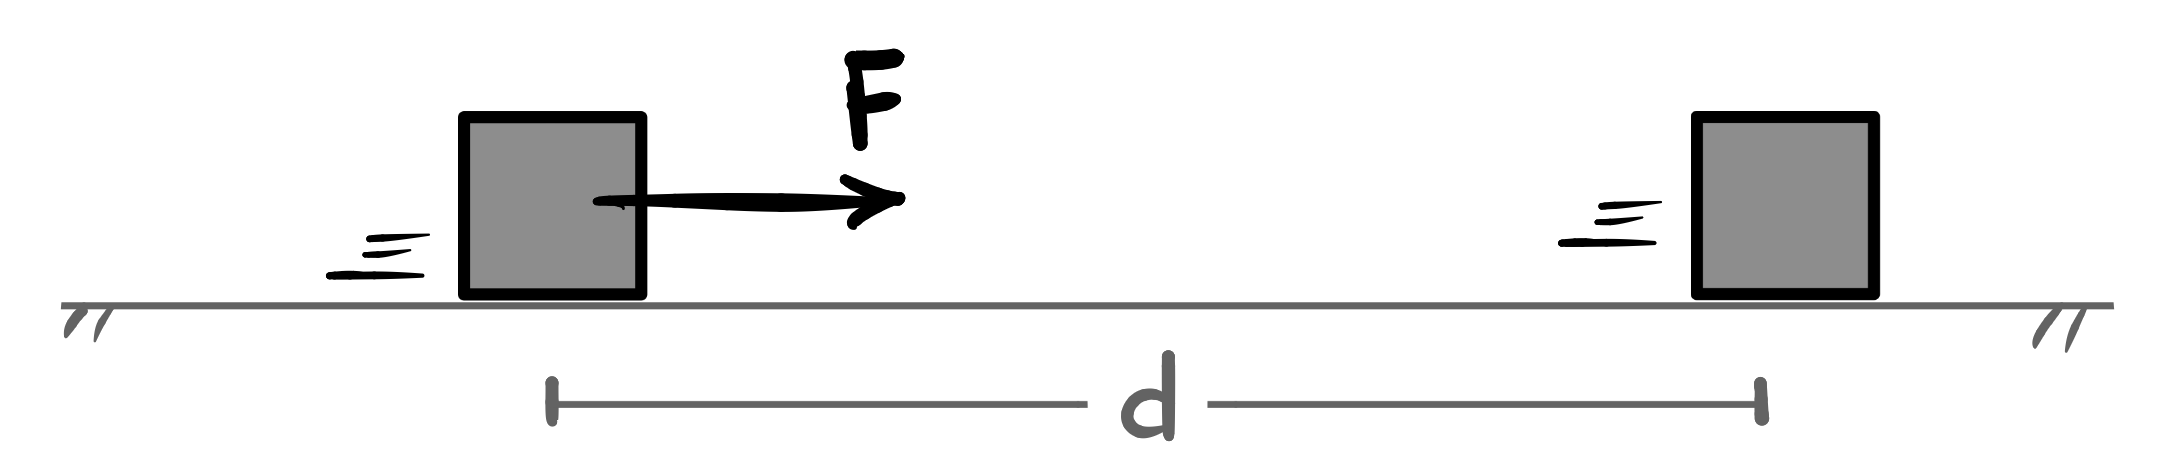
\includegraphics[width=0.6\linewidth]{imagensenergia/trabalhodefinicao3.png}
\captionof{figure}{O efeito da força $F$ sobre o movimento da caixa ao longo do deslocamento $d$ é tão mais intenso quanto maior for o produto $F \cdot d$.}
\label{fig_energia_trabalhodefinicao3}
} 
\vspace{0.3cm}

Sendo assim, é razoável que o leitor concorde que o \emph{efeito gerado sobre o movimento da caixa}\footnote{O que estamos chamando aqui de efeito em breve ganhará um nome mais adequado. Está relacionado à energia injetada na caixa por aquela força. Por enquanto, o leitor pode compreender isto como sendo o \emph{efeito sob o movimento da caixa}, ou seja, quanto maior for o produto $F \cdot d,$ mais velocidade essa caixa ganha devido à ação de tal força.} será tão maior quanto maior for o produto $F \cdot d,$ como mostra a Figura \ref{fig_energia_trabalhodefinicao3}.


 
Há, contudo, uma sutileza geométrica que não pode ser ignorada. Suponha que a
força aplicada seja oblíqua em relação ao deslocamento, como ilustrado na
Figura~\ref{fig_energia_trabalhodefinicao2}. 


\vspace{0.3cm}
{
\centering
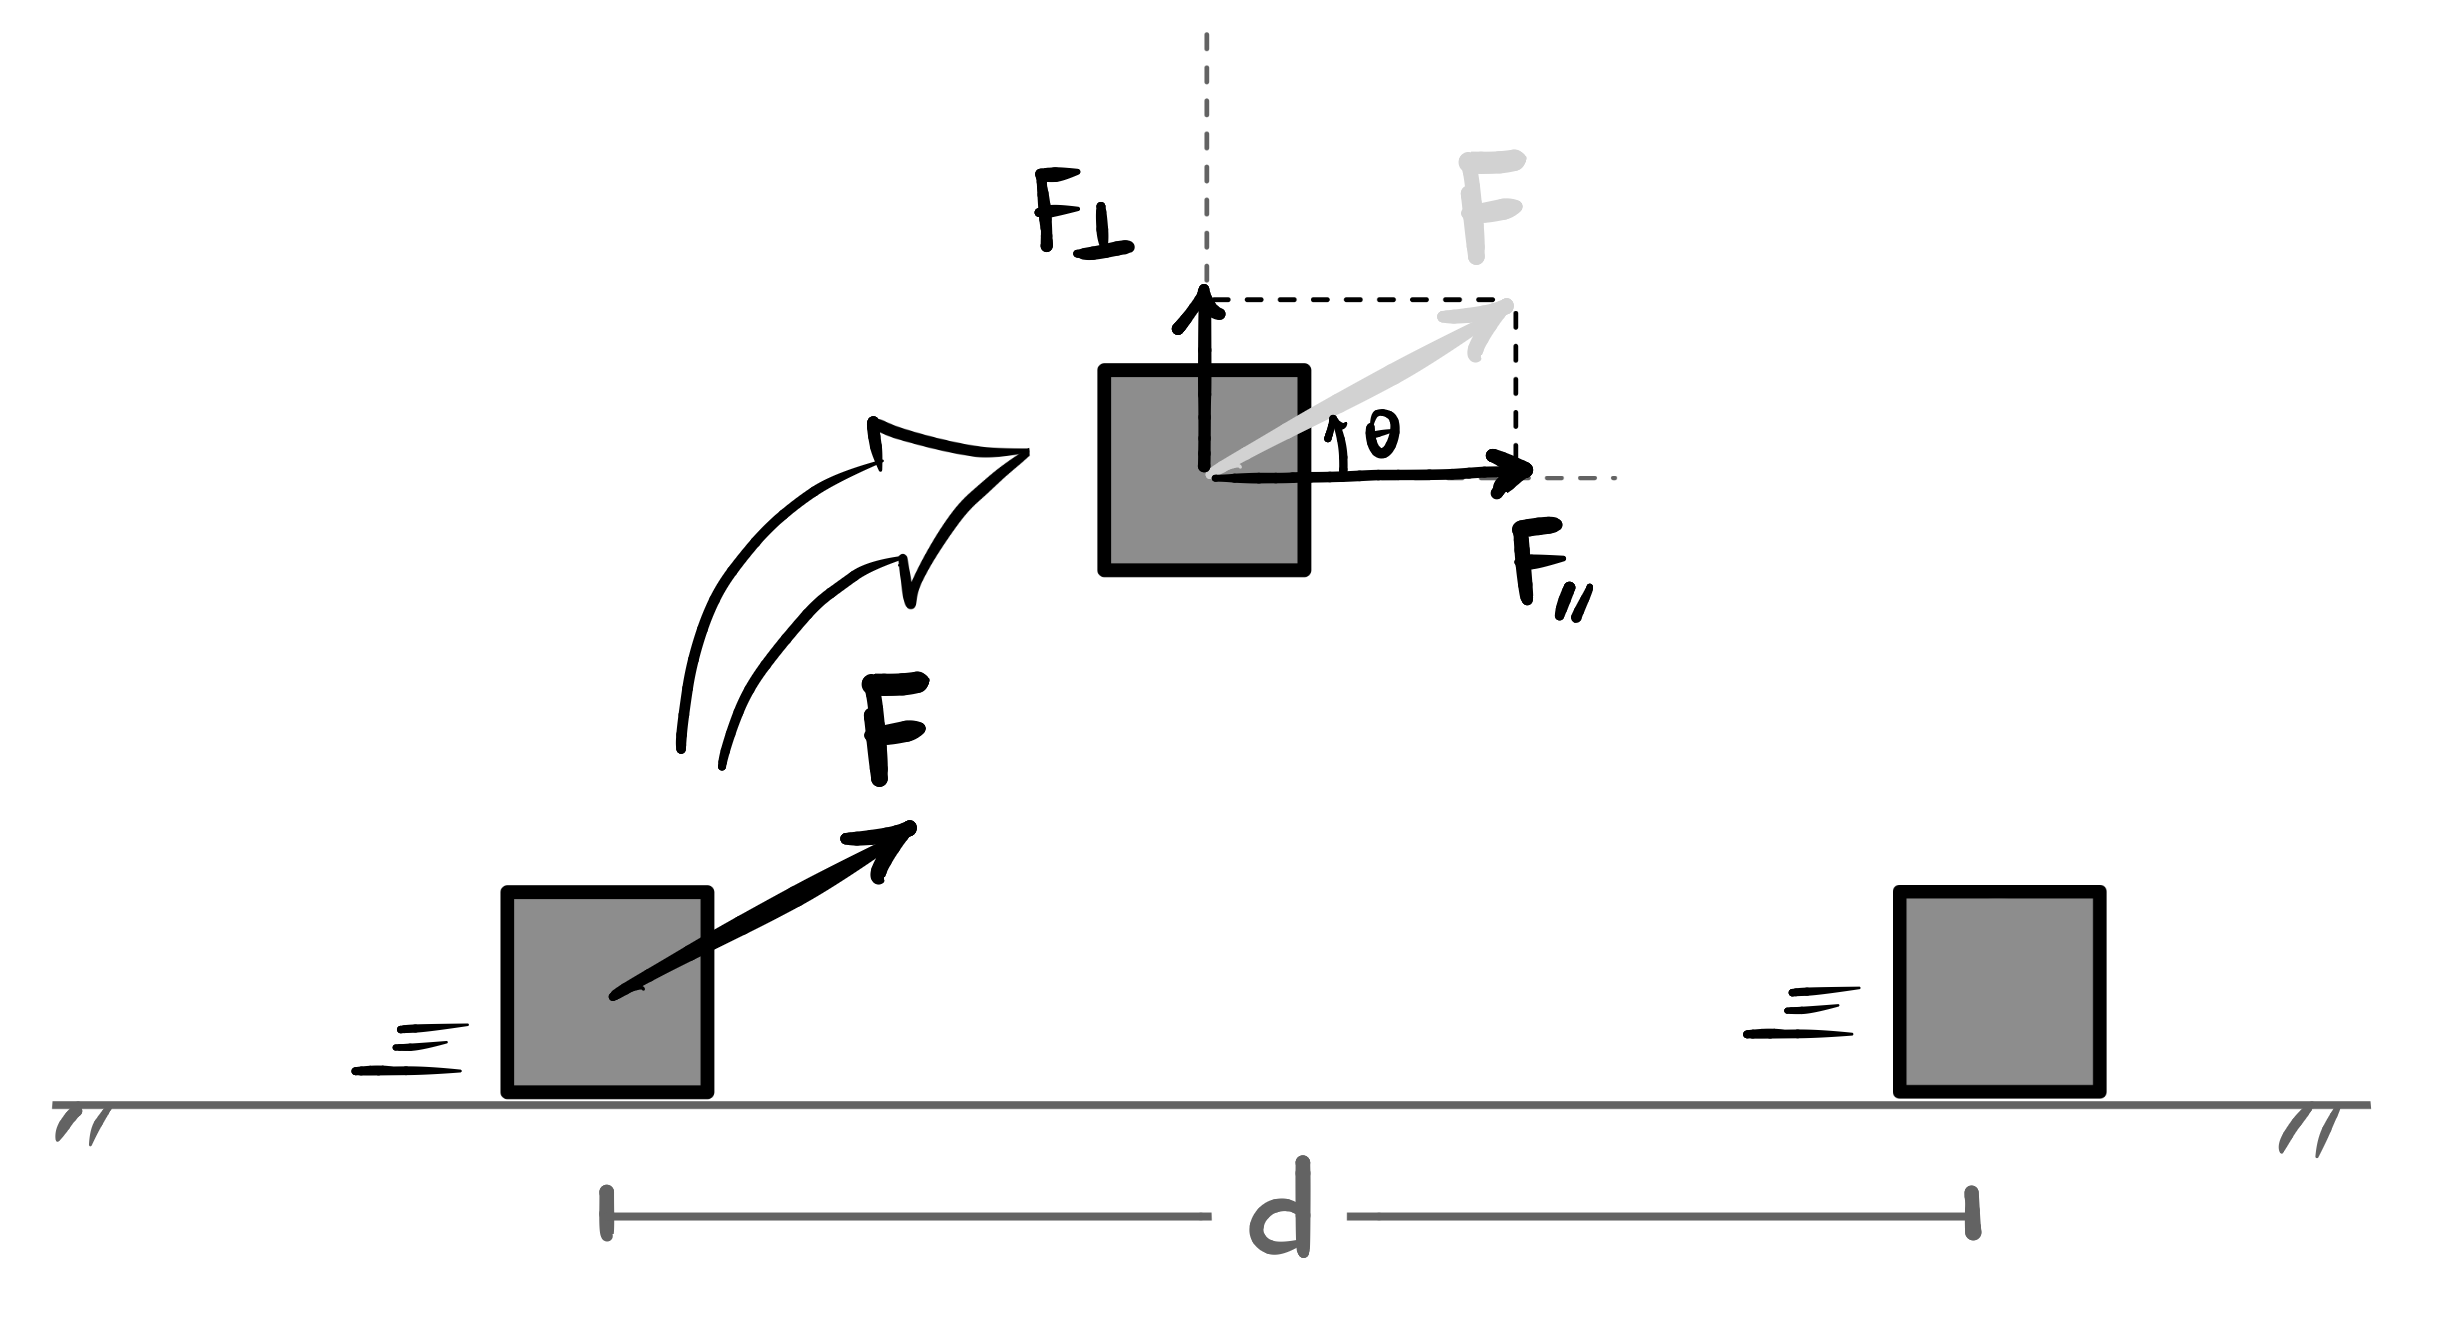
\includegraphics[width=0.5\linewidth]{imagensenergia/trabalhodefinicao2.png}
\captionof{figure}{Uma força oblíqua atuando sobre a caixa possui dois tipos de componentes: $F_{//} $ e $F_{\perp}$.}
\label{fig_energia_trabalhodefinicao2}
} 
\vspace{0.3cm}


A Figura \ref{fig_energia_trabalhodefinicao1} mostra separadamente o mesmo movimento, sob o efeito isolado de cada uma dessas componentes da força $F$. Note, pela primeira imagem, que a componente de força $F_{//}$ é aquela paralela à direção do movimento. É ela, portanto, quem possui a capacidade de alterar a magnitude do movimento -- fazer com que a caixa aumente ou diminua a sua velocidade. 


\vspace{0.3cm}
{
\centering
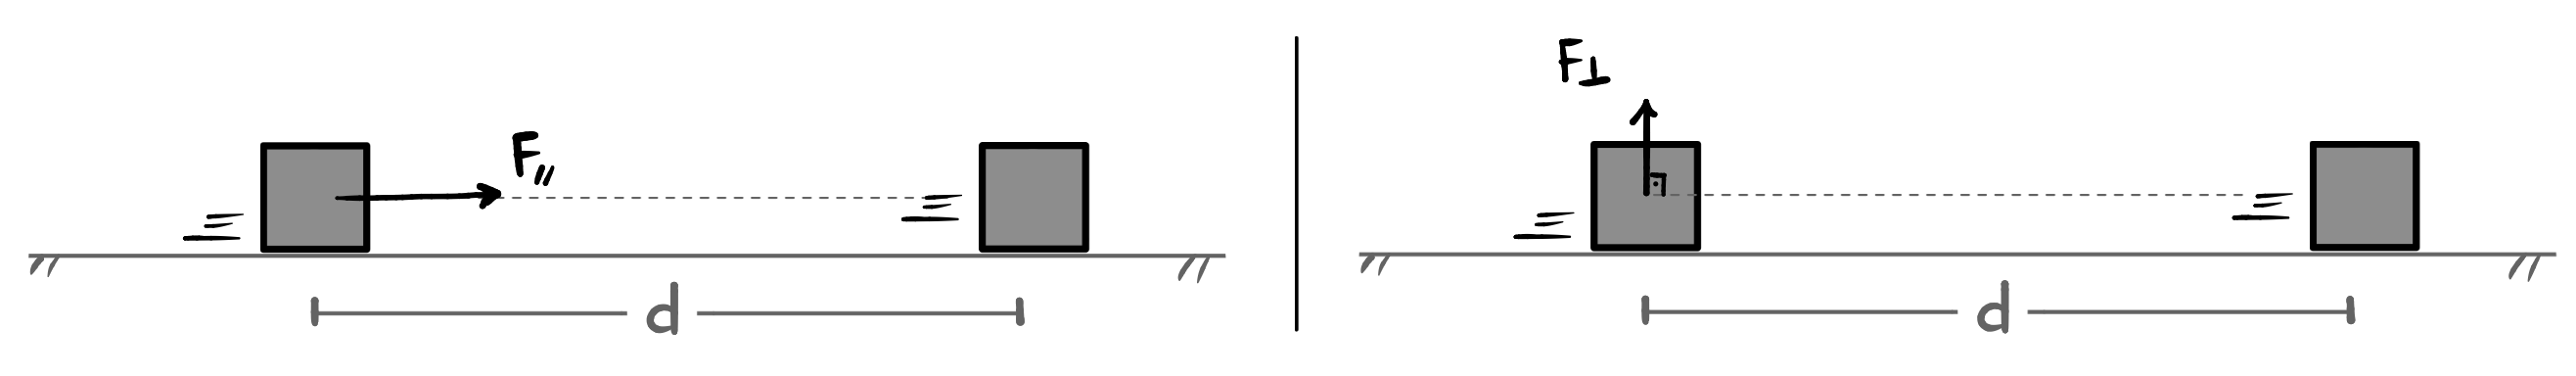
\includegraphics[width=0.8\linewidth]{imagensenergia/trabalhodefinicao1.png}
\captionof{figure}{Apenas a componente da força paralela ao deslocamento é capaz de alterar a magnitude do movimento (velocidade) da partícula.}
\label{fig_energia_trabalhodefinicao1}
} 
\vspace{0.3cm}


A componente $F_{\perp}$, sendo perpendicular à velocidade (e, portanto, perpendicular à direção de movimento) não tem capacidade de alterar a magnitude do movimento. Ela poderia, no máximo -- usando a linguagem de forças -- alterar a direção do movimento, caso agisse como resultante centrípeta. Lembre-se que, neste caso, ela produziria a aceleração centrípeta, responsável por alterar exclusivamente a direção da velocidade, mas não o seu módulo.

Sendo, portanto, apenas a componente de força $F_{//},$ paralela ao deslocamento, responsável por produzir tal deslocamento, dizemos que o \emph{efeito} total de tal força sobre o deslocamento da partícula é, na verdade, o produto $F_{//} \cdot d.$ A esse produto, que vínhamos chamando de \emph{efeito da força sobre o deslocamento,} chamamos de \textit{trabalho da força $F$.} Dizemos que a força $F$ realizou um trabalho sobre a caixa, ao longo do deslocamento $d.$ 

Note que isso é exatamente o que diz a Equação \eqref{eq_energia_trabalho}. A Figura \ref{fig_energia_trabalhodefinicao2} indica o triângulo de vetores decompostos, de onde podemos extrair que $F_{//} = F \cos \theta,$ de onde poderíamos escrever que 

$$ W = F_{//} \cdot d \implies W = F \cdot \cos \theta \cdot d, $$

\noindent que é a mesma equação, porém em um formato mais comum de ser encontrada nos livros de Física. Convido o leitor a notar três casos especiais que merecem atenção imediata:
 
\begin{itemize}
    \item [(i)] Se $\theta = 0^\circ$: a força é paralela ao deslocamento, $\cos 0^\circ = 1$, e o
    trabalho é máximo: $W = Fd$. É exatamente a situação da Figura \ref{fig_energia_trabalhodefinicao3}. Dizemos, nesse caso, que a força \emph{injeta} energia no sistema.
 
    \item [(ii)] Se $\theta = 90^\circ$: a força é perpendicular ao deslocamento,
    $\cos 90^\circ = 0$, e o trabalho é nulo: $W = 0$. Esse é o caso, por exemplo, da
    força normal e da força centrípeta --- ambas perpendiculares ao movimento, ambas
    sem realizar trabalho. Seria exatamente a mesma situação da segunda imagem da Figura \ref{fig_energia_trabalhodefinicao1}: uma força puramente perpendicular à $\vec v.$
 
    \item [(iii)] Se $90^\circ < \theta \leq 180^\circ$: o cosseno é negativo, e o trabalho é
    negativo. Isso ocorre quando a força se opõe ao deslocamento, como no caso da
    força de atrito ou da força de resistência do ar. Dizemos, nesse caso, que a
    força \textit{retira} energia do sistema, daí o seu sinal negativo.
\end{itemize}



 
A unidade de trabalho no SI é o \textbf{joule} (J), em homenagem ao físico inglês
James Prescott Joule (1818--1889), um dos fundadores do estudo da termodinâmica.
Portanto, segue que $1\,\text{J} = 1\,\text{N}\cdot\text{m}$. Essa é a unidade fundamental de energia -- como veremos em breve, trabalho é energia. É a forma sob a qual, através de uma força, podemos imprimir ou retirar energia de um sistema.

Note que o trabalho é, portanto, um número real --- uma grandeza \textbf{escalar}
---, ainda que seja construído a partir de duas grandezas vetoriais (a velocidade da partícula e a força que nela atua). O trabalho não aponta para lugar nenhum. Ele já é construído com base nas componentes de forças que apontam na direção do deslocamento.

A essa altura, pode parecer não ter sentido nenhum construir essa grandeza, mas, como veremos em breve, o trabalho será o meio pelo qual conseguiremos retirar ou adicionar \emph{energia} em um sistema. Essa própria grandeza -- a tal da energia -- será detalhada e estudada nas próximas equações.



\secgfe{Onde é usada}


O conceito de trabalho -- o alicerce da formulação escalar da dinâmica -- será central em todo o estudo daqui em diante. Todas as demais equações dessa seção envolverão, de forma explícita ou implícita, o conceito de trabalho.

O conceito de energia potencial -- que dá origem ao teorema da conservação da energia mecânica -- é construído com base na definição de trabalho. A forma específica com que definiremos energia cinética, na Equação \eqref{eq_energia_energiacinetica}, será feita daquela maneira por conta do conceito de trabalho, como ficará claro no desenvolvimento da Equação \eqref{eq_energia_teoremaenergiacinetica}, que relaciona essas duas grandezas no teorema da energia cinética.

Assim, o conceito de trabalho é central em toda a formulação escalar da dinâmica: ele é o alicerce sob o qual construiremos os demais conceitos e equações. Seria o análogo do conceito de força na formulação newtoniana: as forças são o alicerce -- o agente fundamental responsável por gerar a aceleração, que varia o movimento do corpo. Na formulação dinâmica, o \emph{trabalho de uma força} é quem ocupa este lugar: será ele o responsável pela variação da magnitude do movimento, como veremos em breve.





\secgfe{Erros comuns}

O erro mais comum é apenas multiplicar a força $F$ pelo deslocamento $d$ para computar o trabalho, fazendo $W= F\cdot d$, enquanto na verdade é preciso pegar a componente $F_{//}$ da força paralela à direção do deslocamento $d$: $W= F_{//} \cdot d.$ A diferença é sutil, mas muda tudo.

Considere, por exemplo, a situação da Figura \ref{fig_energia_trabalhoerroscomuns1}, que mostra um bloco que se desloca horizontalmente ao longo de uma superfície. Sendo sua massa $m=3$ kg, qual é o valor do trabalho da força normal quando o bloco se desloca por 10 metros?

\vspace{0.3cm}
{
\centering
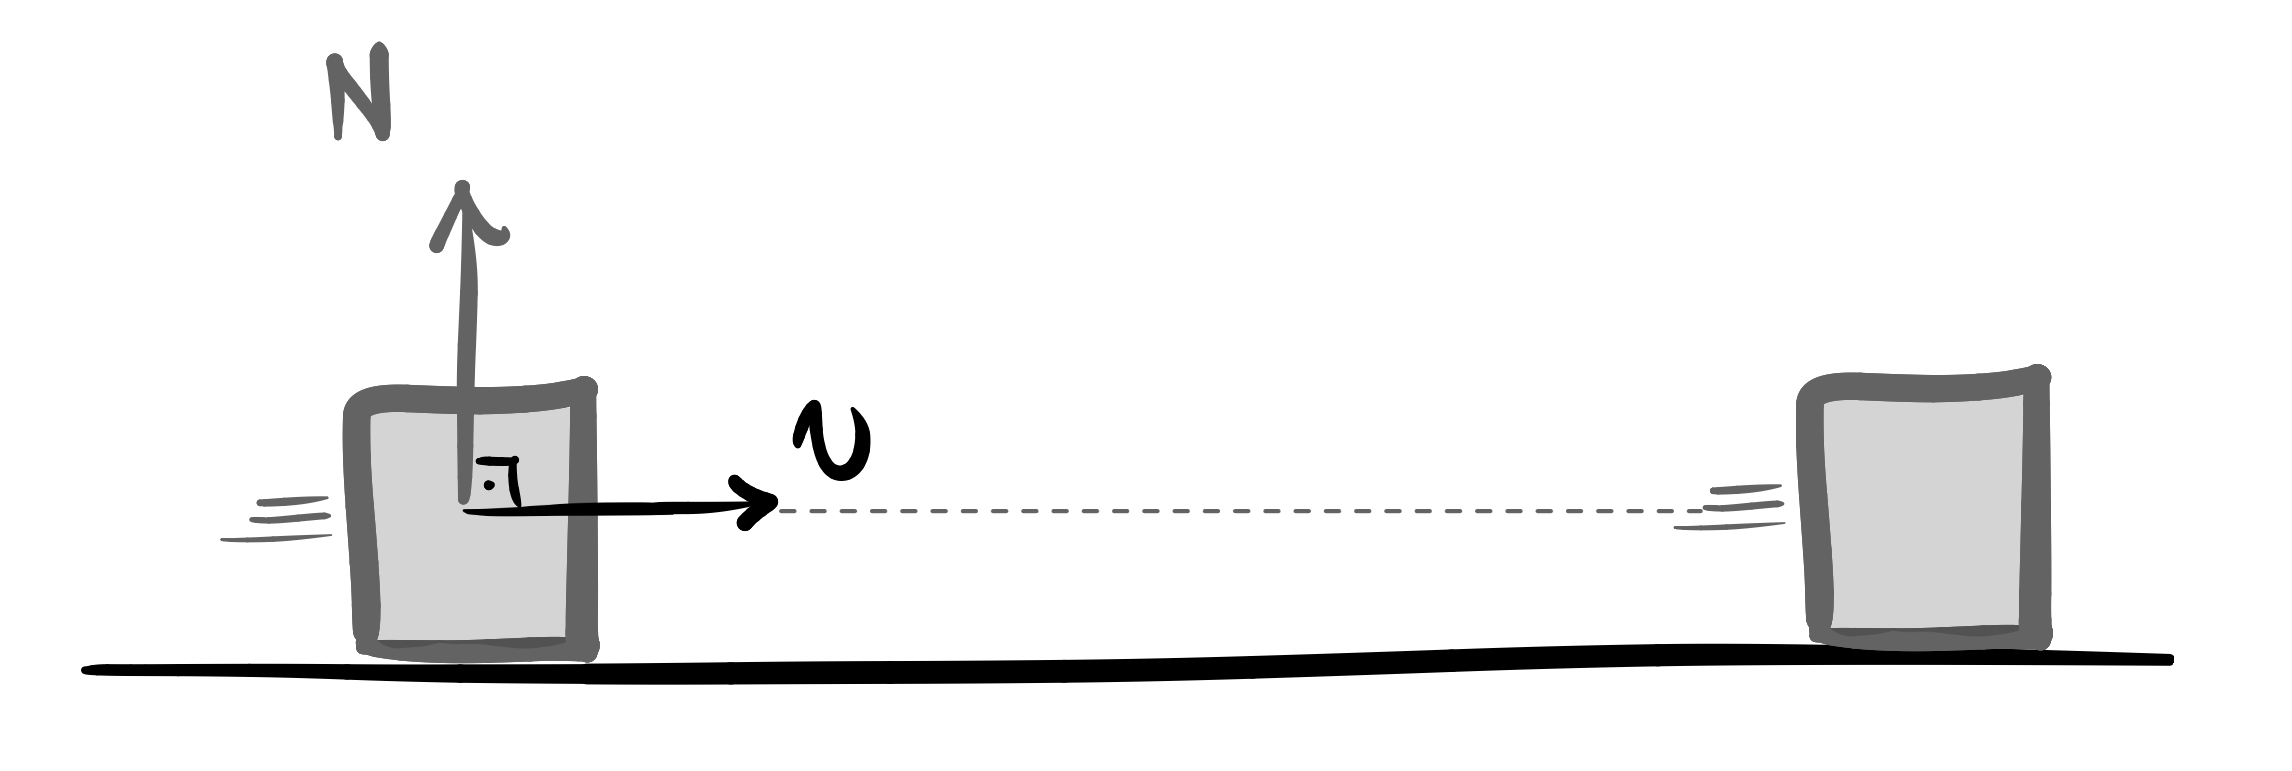
\includegraphics[width=0.55\linewidth]{imagensenergia/trabalhoerroscomuns1.png}
\captionof{figure}{Forças perpendiculares à direção de deslocamento não realizam trabalho.}
\label{fig_energia_trabalhoerroscomuns1}
} 
\vspace{0.3cm}


Ora, a normal é igual ao peso, haja vista que o bloco está em equilíbrio na vertical, logo, $N=P=mg=30$N. Assim, o trabalho da força normal que o solo faz sob o bloco seria

$$ W_\text{N} = N \cdot d = 30 \cdot 10 = 300 \text{ J.}$$

Isso, contudo, está errado. Veja que a componente da força normal (que é vertical) na direção do deslocamento (que é horizontal) é nula, isto é, $N_{//} = 0.$ A força normal, portanto, não realiza trabalho: $W_\text{N} = 0.$

Sempre que uma força é perpendicular à velocidade do corpo (e, portanto, perpendicular à direção de deslocamento) ela não irá realizar trabalho, haja vista que $F_{//} = 0:$ a força não possui componente paralela à direção do deslocamento (que é a direção do vetor velocidade $\vec v$ da partícula), haja vista que ela é perpendicular a tal direção. Assim, o trabalho da tração quando o bloco vai da posição $A$ até a posição $B$ no movimento pendular da Figura \ref{fig_energia_trabalhoerroscomuns2} é, também, nulo: a tração é sempre perpendicular à velocidade, de modo que $T_{//} = 0.$


\vspace{0.3cm}
{
\centering
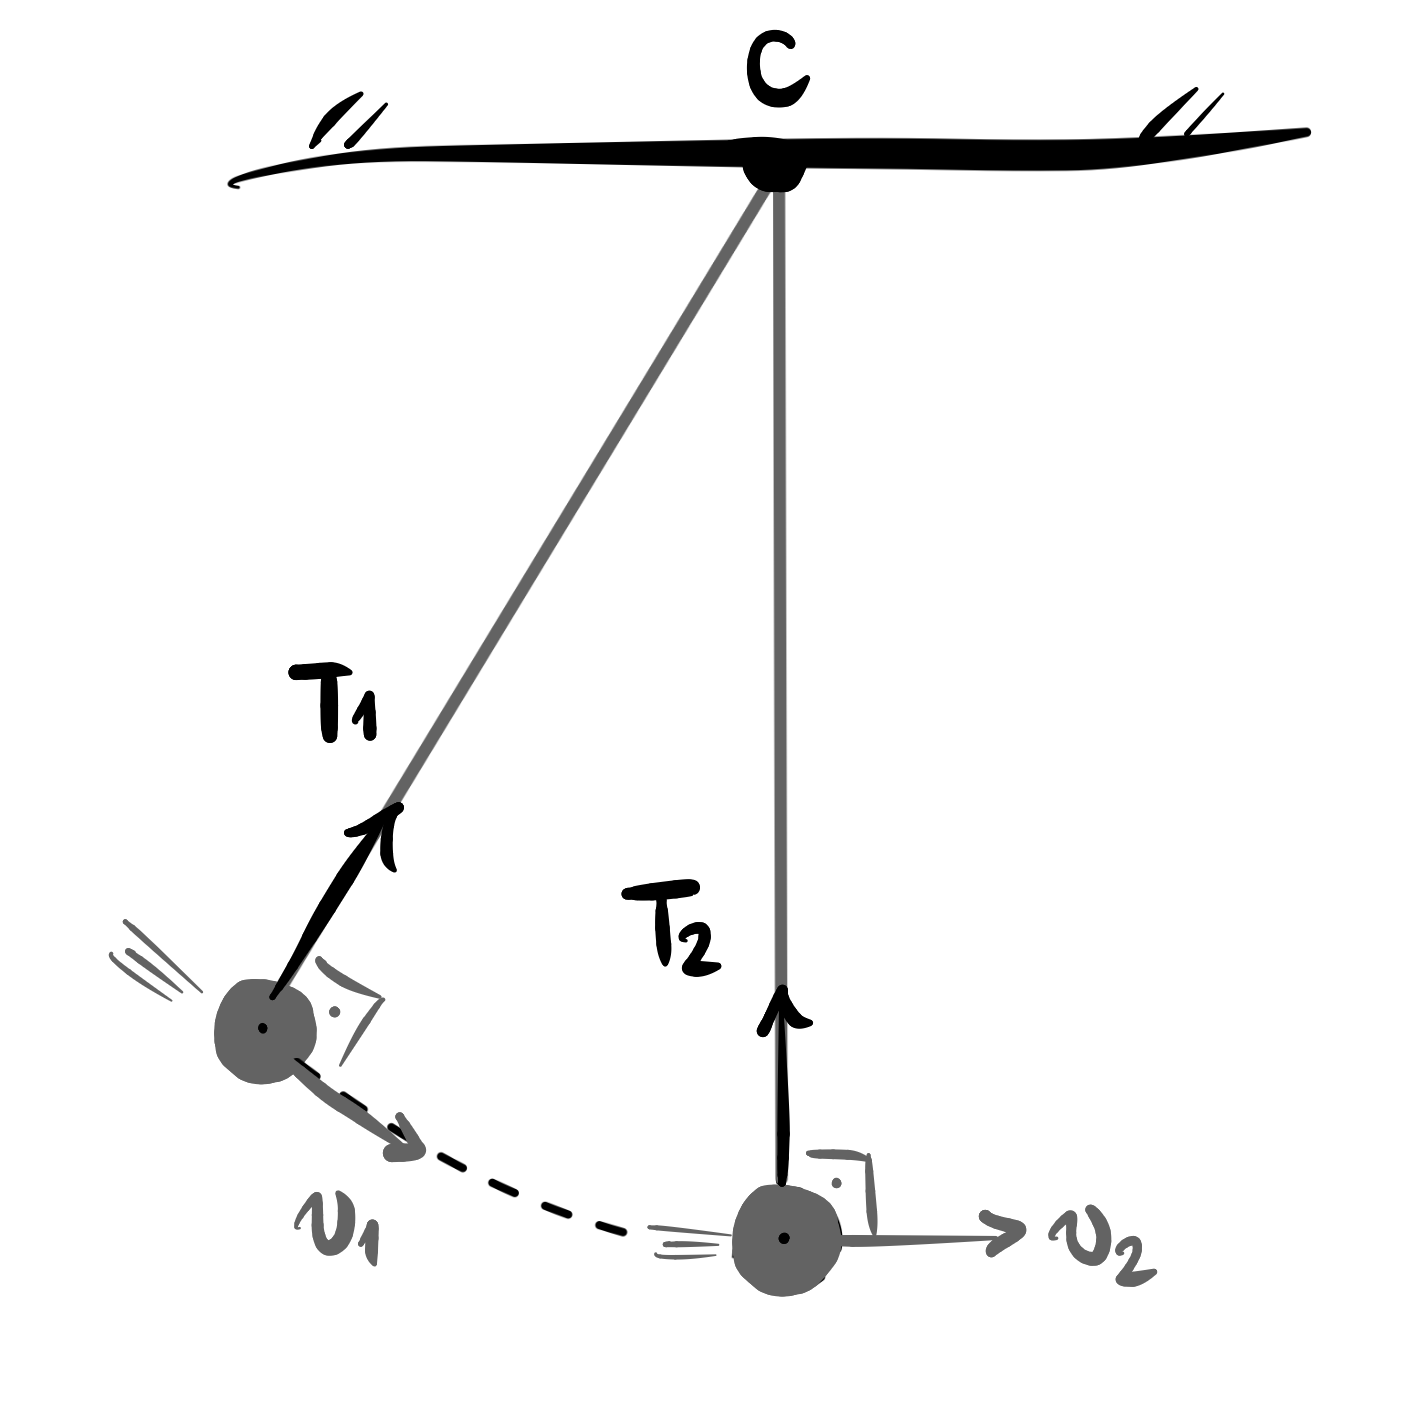
\includegraphics[width=0.35\linewidth]{imagensenergia/trabalhoerroscomuns2.png}
\captionof{figure}{O trabalho da tração.}
\label{fig_energia_trabalhoerroscomuns2}
} 
\vspace{0.3cm}



\secgfe{Observações}


A Equação~\eqref{eq_energia_trabalho} foi construída sob a hipótese de que a força é
constante ao longo do deslocamento. Mas o leitor já conhece, ao menos, uma força
que não satisfaz essa condição: a força elástica de uma mola, dada pela Lei de
Hooke, $F = kx$, cresce linearmente com a deformação e, portanto, \textit{muda de
valor a cada ponto} do percurso. Como calcular o trabalho nesse caso?
 
O caminho não é difícil, mas exige uma mudança de perspectiva. Considere a situação
da Figura~\ref{fig_energia_trabalhoforcaelastica}: a mola é comprimida de $x_0$ e, ao ser solta,
empurra um bloco da posição $x = x_0$ até a posição natural $x = 0$. À medida que o
bloco se move, a força que a mola exerce sobre ele diminui --- de $kx_0$ no início
a zero no final. Não podemos, portanto, multiplicar ``a força'' pelo deslocamento:
\textit{não há uma única força} ao longo do percurso.

 O leitor já conhece essa situação, é a mesma discutida no Apêndice \ref{apendice_areagraficovxt}: neste caso, o trabalho é computado pela área abaixo do gráfico da força pelo deslocamento.

\vspace{0.3cm}
{
\centering
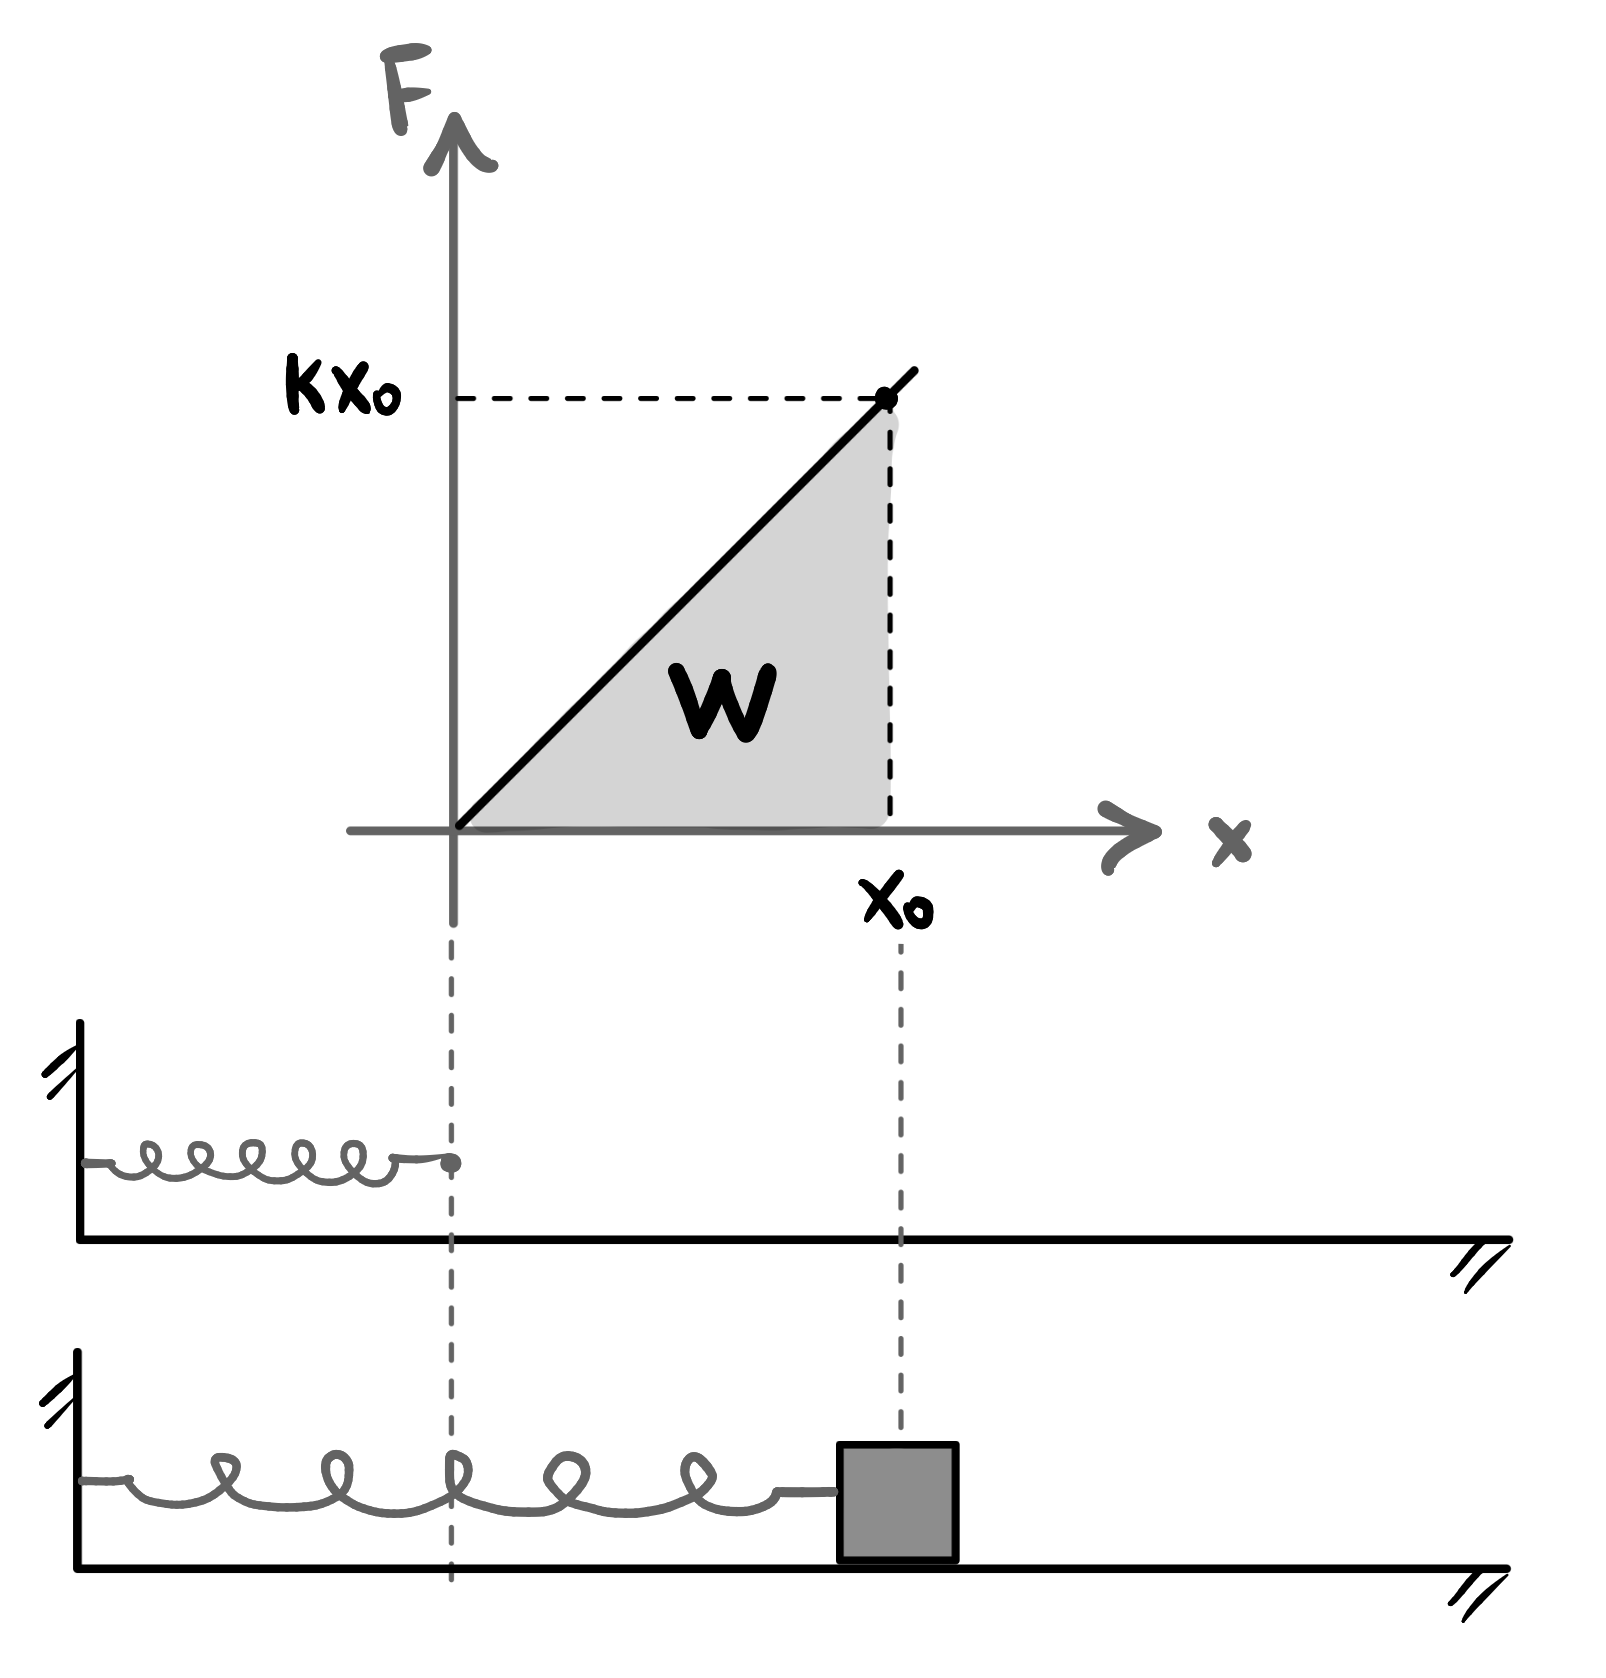
\includegraphics[width=0.5\linewidth]{imagensenergia/trabalhoforcaelastica.png}
\captionof{figure}{O trabalho da força elástica.}
\label{fig_energia_trabalhoforcaelastica}
} 
\vspace{0.3cm}


 
Para a força elástica $F(x) = kx$, o gráfico $F \times x$ é uma reta que parte da
origem, como mostra a Figura \ref{fig_energia_trabalhoforcaelastica}. A área sob essa reta, de $x = 0$ até $x = x_0$, é um triângulo de base $x_0$ e altura $kx_0$:
%
\begin{equation*}
    W_{\text{elást}} = \frac{1}{2} \cdot x_0 \cdot kx_0 = \frac{1}{2}kx_0^2.
\end{equation*}
%
Esse resultado --- que o leitor encontrará novamente na Equação~\eqref{eq_energia_potencialelastica},
ao estudar a energia potencial elástica --- não poderia ser obtido simplesmente
por $W = F \cdot d$, pois não existe um valor único de $F$ ao longo do percurso. Assim, quando a mola puxa a caixa de $x_0$ até $x=0$ -- seu comprimento natural -- a quantidade de energia (o trabalho feito pela mola) que ela injeta na caixa é igual a $\sfrac{kx_0^2}{2}.$
 
A mesma lógica se aplica a qualquer força variável paralela à direção do deslocamento: seu trabalho, ao deslocar um corpo de $x_1$ até $x_2,$ será igual à área abaixo do gráfico $F(x)$, entre $x_1$ e $x_2.$
 
% Há uma observação final que merece destaque: quando a força é negativa em um certo
% intervalo (ou seja, aponta em sentido contrário ao deslocamento), a ``área'' sob a
% curva nesses trechos é \textit{negativa} --- geometricamente, a curva fica abaixo
% do eixo $x$. O trabalho total é, então, a \textbf{área algébrica}: soma das áreas
% positivas com as áreas negativas, levantando em conta seus sinais. É por esse motivo, aliás, que o trabalho do
% atrito é negativo: seu gráfico $F \times x$ é uma reta horizontal \textit{abaixo}
% do eixo, e sua área é, portanto, negativa por definição.




\vspace{0.3cm}

\begin{exemplo}[Nível I]\label{exemplo_energia_trabalhoex01}


Um operário empurra uma caixa ao longo de um corredor horizontal liso, aplicando
uma força horizontal constante de $80\,\text{N}$ por uma distância de $5\,\text{m}$.
Qual é o trabalho realizado por essa força?

\resolucao

A força aplicada é horizontal e o deslocamento também é horizontal, de modo que o
ângulo entre eles é $\theta = 0°$. Aplicando diretamente a definição de trabalho:
%
\begin{equation*}
    W = F\cos\theta \cdot d = 80 \cdot \cos 0° \cdot 5 = 80 \cdot 1 \cdot 5
    = \boxed{400\,\text{J}.}
\end{equation*}
 
Note que a massa da caixa não foi necessária para o cálculo --- ela seria relevante
se precisássemos calcular a aceleração produzida pela força, mas o trabalho depende
apenas da força, do deslocamento e do ângulo entre eles: ele representa o quanto de energia foi injetada na caixa, o que a faz ganhar mais movimento. Quanto de velocidade esse ganho de energia representa será algo que discutiremos nas próximas seções.

\end{exemplo}


\vspace{0.3cm}





\begin{exemplo}[Nível II]\label{exemplo_energia_trabalhoex02}

Um bloco de $4\,\text{kg}$ é puxado a partir do repouso ao longo de uma superfície
horizontal rugosa por uma força $F = 30\,\text{N}$ que faz um ângulo de $37^\circ$ com a
horizontal. O coeficiente de atrito cinético entre o bloco e a superfície é
$\mu_c = 0{,}25$. Calcule o trabalho realizado por cada força que age sobre o bloco
ao longo de um deslocamento de $6\,\text{m}$, e determine o trabalho total.
Adote $g = 10\,\text{m/s}^2$, $\cos 37^\circ = 0{,}8$ e $\sin 37^\circ = 0{,}6$.

\resolucao

O primeiro passo é identificar todas as forças que atuam sobre o bloco: o peso
$\vec{P}$, a normal $\vec{N}$, a força aplicada $\vec{F}$ e a força de atrito
$\vec{F}_\text{AT}$. 



\vspace{0.3cm}
{
\centering
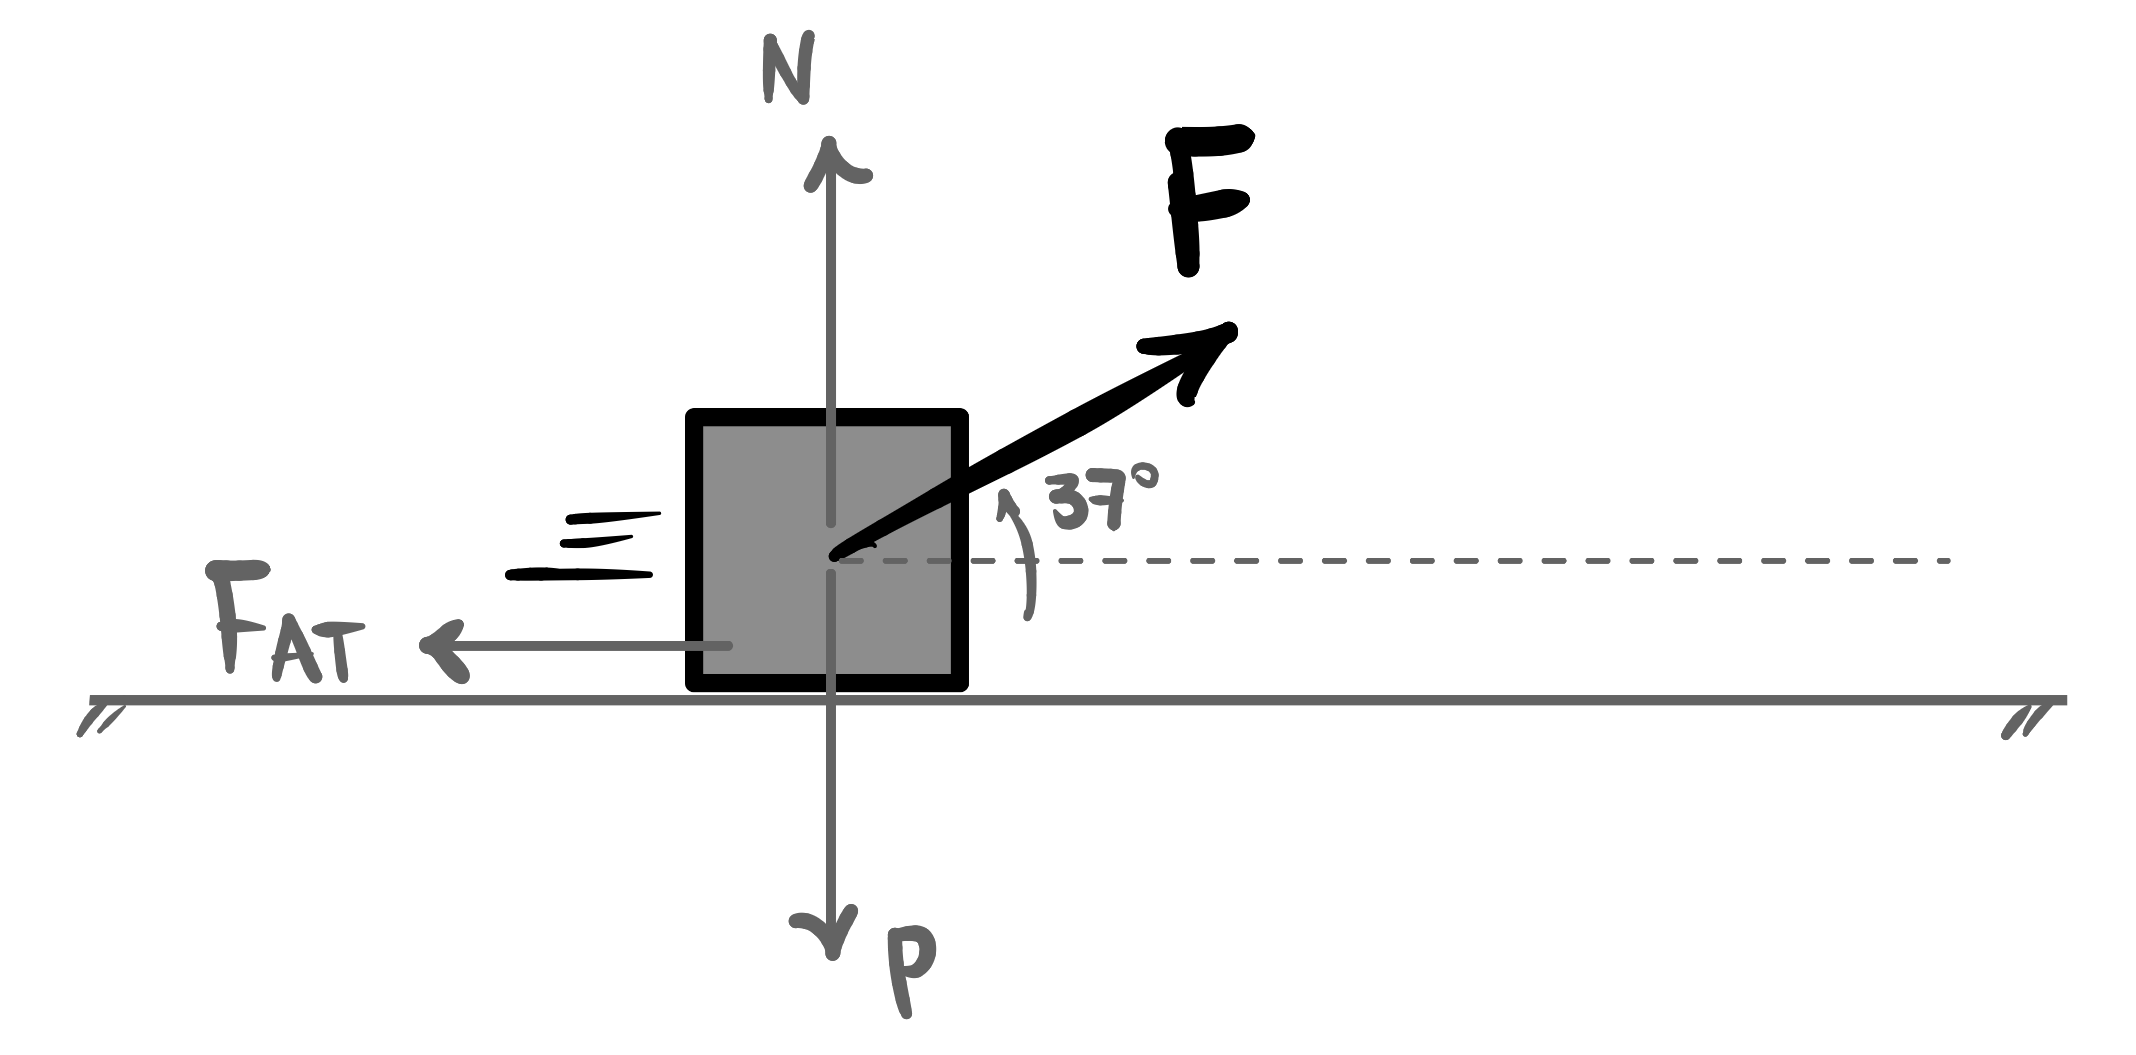
\includegraphics[width=0.4\linewidth]{imagensenergia/trabalhoexemplonivel2.png}
\captionof{figure}{}
\label{fig_energia_trabalhoexemplonivel2}
} 
\vspace{0.3cm}



A Figura \ref{fig_energia_trabalhoexemplonivel2} ilustra o diagrama de forças. Avaliemos cada uma delas separadamente. \\
 
\textbf{Peso e normal:} Ambos são perpendiculares ao deslocamento horizontal

($\theta = 90^\circ$), portanto:
%
\begin{equation*}
    W_P = 0 \qquad \text{e} \qquad W_N = 0.
\end{equation*}
 
\textbf{Força aplicada:} a componente paralela ao deslocamento é
$F_{//} = F\cos 37^\circ = 30 \cdot 0{,}8 = 24\,\text{N}$. Logo:
%
\begin{equation*}
    W_F = F\cos 37^\circ \cdot d = 24 \cdot 6 = 144\,\text{J}.
\end{equation*}
 
\textbf{Força de atrito:} para calculá-la, precisamos da normal. O equilíbrio
vertical do bloco exige que $F_{\text{R}_y}=0,$ ou seja:
%
\begin{equation*}
    N + F\sin 37^\circ = mg \implies N = mg - F\sin 37^\circ = 40 - 30 \cdot 0{,}6
    = 40 - 18 = 22\,\text{N}.
\end{equation*}
%
Note que a componente vertical da força aplicada \textit{reduz} a normal,
diminuindo assim o atrito. A força de atrito cinético é:
%
\begin{equation*}
    F_\text{AT} = \mu_c N = 0{,}25 \cdot 22 = 5{,}5\,\text{N},
\end{equation*}
%
e seu trabalho, sendo ela oposta ao movimento ($\theta = 180^\circ$), é:
%
\begin{equation*}
    W_{\text{F}_{AT}} = -F_\text{AT} \cdot d = -5{,}5 \cdot 6 = -33\,\text{J}.
\end{equation*}
 
\textbf{Trabalho total:}
%
\begin{equation*}
    W_{\text{total}} = W_F + W_{\text{F}_{AT}} + W_P + W_N = 144 + (-33) + 0 + 0
    = \boxed{111\,\text{J}.}
\end{equation*}

Isso representa a \emph{energia total} que foi injetada no sistema: 144J foram injetados, 33J dissipados, e o resultado líquido foram $111$J de energia que a caixa ganhou -- o que se converteu em um aumento do seu movimento (sua velocidade). Note que somar os trabalhos é tarefa simples: é simplesmente somar números. Não é necessário se preocupar com direção, ângulos e decomposições -- essa é a vantagem de se trabalhar com grandezas escalares em relação às vetoriais.

\end{exemplo}


\vspace{0.3cm}





\begin{exemplo}[Nível III]\label{exemplo_energia_trabalhoex03}

Uma caixa de massa $m$ é empurrada para cima ao longo de um plano inclinado de
ângulo $\alpha$ e comprimento $L$, com coeficiente de atrito cinético $\mu_c$.
A força aplicada é paralela ao plano. Ao chegar ao topo, a caixa é abandonada e
desliza de volta até a base. Determine:
\begin{enumerate}
    \item [a)] O trabalho total realizado pelo atrito ao longo do percurso completo
    (subida + descida).
    \item [b)] O trabalho total realizado pelo peso ao longo do percurso completo.
    \item [c)] Para que valores de $\mu_c$ a caixa \emph{não} retorna espontaneamente
    após ser abandonada no topo?
\end{enumerate}

\resolucao

\textit{a)} Trabalho do atrito.
 
A força de atrito cinético tem módulo $F_\text{AT} = \mu_c mg\cos\alpha$ em qualquer ponto
do percurso. O que muda entre a subida e a descida é a \textit{direção} do atrito
--- ele sempre se opõe ao movimento. Assim, o vetor $F_\text{AT}$ faz sempre $180^\circ$ com a velocidade $\vec v,$ e, portanto, em ambos os trechos o atrito realiza trabalho
\textit{negativo}:
%
\begin{align*}
    W_{F_{AT},\,\text{subida}}  &= -\mu_c mg\cos\alpha \cdot L, \\
    W_{F_{AT},\,\text{descida}} &= -\mu_c mg\cos\alpha \cdot L.
\end{align*}
 
O trabalho total do atrito no percurso completo é, portanto:
%
\begin{equation*}
     \boxed{W_{F_{AT}} =-2\mu_c mgL\cos\alpha.}
\end{equation*}
 
O sinal é sempre negativo, independentemente do sentido do movimento: o atrito é
uma força dissipativa e \textit{sempre} retira energia do sistema. \\
 
\textit{b)} Trabalho do peso:
 
O peso realiza trabalho negativo na subida (a componente $P_{//} = P \sin \alpha$ se opõe à velocidade neste trecho, ou seja, $\theta = 180^\circ$) e positivo na descida (a componente $P_{//} = P \sin \alpha$ está na mesma direção e sentido de $\vec v$ neste trecho, ou seja, $\theta = 0^\circ$):
%
\begin{align*}
    W_{P,\,\text{subida}}  &= -(mg \sin\alpha )L, \\
    W_{P,\,\text{descida}} &= + (mg \sin\alpha)L.
\end{align*}
 
O trabalho total do peso é:
%
\begin{equation*}
    \boxed{W_P = -mgL\sin\alpha + mgL\sin\alpha = 0.}
\end{equation*}
 
Em breve veremos que forças desse tipo são chamadas de \textit{conservativas}: o trabalho que realiza em um percurso de
ida e volta é sempre nulo, independentemente do caminho percorrido. Voltaremos a
esse conceito ao estudar a energia potencial gravitacional -- o peso será uma força deste tipo. \\
 
\textit{c)} Condição para que a caixa não retorne:
 
Para que a caixa não deslize de volta ao ser abandonada no topo, o atrito estático
deve ser capaz de equilibrar a componente do peso ao longo do plano. Usando
$\mu_e \approx \mu_c$, a condição é:
%
\begin{equation*}
    mg\sin\alpha \leq \mu_c\, mg\cos\alpha \implies \boxed{\mu_c \geq \tan\alpha,}
\end{equation*}

\noindent exatamente aquela construída no desenvolvimento da Equação \eqref{eq_dinamicanewtoniana_gsintheta}. Para planos com inclinação $\alpha$, é necessário que o coeficiente de atrito seja
ao menos igual a $\tan\alpha$ para que a caixa permaneça parada no topo.



\end{exemplo}


\vspace{0.3cm}











\begin{secnivel}[Energia Cinética]{I}{Energia Cinética}
 

  \eqLdois{def}{eq_energia_energiacinetica}{E_\text{C} := \dfrac{1}{2}mv^2}
  
\end{secnivel}







\secgfe{De onde vem}

Quando este que vos escreve iniciou seus estudos de Física, ainda adolescente, durante o ensino médio, foi tomado por uma terrível sensação: a de que o tempo inteiro os físicos inventavam grandezas, davam nomes estranhos e criavam complicadas fórmulas matemáticas para os tais conceitos inventados, sem nenhum tipo de razão clara aparente. A fim de não causar sensação semelhante ao leitor, essa subseção será, talvez, mais longa que o habitual. Mas trará um pouco de história de modo a deixar o mais evidente, claro e intuitivo que se possa a razão de criar a grandeza dada pela Equação \eqref{eq_energia_energiacinetica}. Se o autor há de lograr êxito nessa empreitada, deixo para julgamento do leitor, ao fim da seção. Vamos aos fatos.

\subsubsection*{O problema}

Um objeto em movimento possui algo que um objeto em repouso não possui. Isso é óbvio -- o que não é óbvio é como medir esse ``algo'' com precisão.
 
Vamos formular a pergunta de maneira mais precisa: \emph{quando um corpo em movimento
colide contra uma parede e para, que grandeza física determina o estrago causado?}
 
Estamos perguntando, em outras palavras: qual é a medida correta do ``potencial
destrutivo'' de um objeto em movimento? Essa pergunta foi o
epicentro de uma das maiores controvérsias da história da física, que envolveu os maiores
nomes do século XVII e XVIII, e sua resposta é precisamente o que chamamos hoje de
energia cinética.
 
As duas candidatas naturais à resposta eram:
 
\begin{itemize}
    \item [(i)] A grandeza $mv$ -- proposta pelo francês Descartes, que a chamava de
          \textit{quantidade de movimento}. É exatamente aquilo que estudamos na Equação \eqref{eq_newton_momentolinear}.
    \item [(ii)] A grandeza $mv^2$ -- proposta pelo alemão Leibniz, que a chamava de
          \textit{vis viva} (força viva).
\end{itemize}
 
\noindent Ambas dependem da massa e da velocidade. Qual das duas mede o estrago?
E por quê?
 
%-------------------------------------------------------------
\subsubsection*{O experimento da argila}
 
Por volta de 1722, o físico holandês Willem Jacob \mbox{'s~Gravesande} realizou um
experimento que, com o benefício do tempo, parece conclusivo. Ele deixava cair bolas de
bronze de diferentes massas e de diferentes alturas sobre uma placa de argila mole,
e media a profundidade da marca deixada por cada bola.
 
A pergunta experimental era precisa: se dobrarmos a velocidade de impacto, a marca
na argila dobra, quadruplica, ou segue outra lei?
 
O leitor poderia tentar responder antes de prosseguir. Se a grandeza relevante fosse
$mv$, dobrar a velocidade dobraria $mv$ e, esperaríamos, dobraria o estrago. Se fosse
$mv^2$, dobrar a velocidade quadruplicaria $mv^2$ e, esperaríamos, quadruplicaria
o estrago.\footnote{É natural que, quanto maior fosse a massa $m$ de um corpo, maior seria o estrago para uma mesma velocidade de impacto, razão pela qual a massa $m$ aparece nas duas expressões.}
 
Os dados obtidos foram inequívocos: \textit{a profundidade da marca era
proporcional ao quadrado da velocidade}, não à velocidade. Ao dobrar a velocidade de
impacto, a marca na argila quadruplicava. Ao triplicar a velocidade, a marca tornava-se
nove vezes mais profunda. O estrago seguia $v^2$, não $v$. Leibniz tinha razão, e Descartes estava errado (ao menos nesse aspecto).
 
Mas como Gravesande controlava a velocidade das bolas? Afinal, é difícil
lançar uma bola com velocidade exatamente conhecida. A solução foi elegante: ele não
lançava as bolas horizontalmente — ele as \textit{deixava cair de alturas variadas}.
Galileu já havia demonstrado (e o leitor conhece este problema) que a velocidade
adquirida em queda livre a partir do repouso satisfaz:
 
\[
    v^2 = 2gh \implies h = \frac{v^2}{2g}
\]
 
\noindent Portanto, a altura de queda é proporcional ao quadrado da velocidade
de impacto. Ao variar a altura, Gravesande variava $v^2$ de forma controlada
e conhecida.
 
O resultado observado foi:
 
\[
    \text{profundidade da marca} \;\propto\; h \;\propto\; v^2
\]
 
\noindent A grandeza que determina o estrago, portanto, é $mv^2$, não $mv$.
 
%-------------------------------------------------------------
\subsubsection*{Por que $mv$ falha: o argumento das bolas gêmeas}
 
Existe uma forma ainda mais direta de ver por que $mv$ não pode ser a medida certa do
``potencial destrutivo''. Considere o seguinte experimento mental.
 
Temos duas bolas, $A$ e $B$. A bola $A$ tem massa $4m$ e velocidade $v$. A bola $B$ tem massa $m$
e velocidade $4v$. As duas têm exatamente o mesmo momento linear:
 
\[
    p_A = 4m \cdot v = 4mv \qquad \text{ e } \qquad p_B = m \cdot 4v = 4mv.
\]
 
\noindent Se $mv$ fosse a medida do estrago, as duas bolas deveriam causar marcas
idênticas na argila. Mas lançá-las mentalmente contra uma parede basta para sentir que
algo está errado: a bola $B$, quatro vezes mais rápida, deve ser muito mais ``perigosa''
do que a bola $A$, quatro vezes mais lenta e pesada.\footnote{Imagine uma bala de revólver -- alta velocidade e pequena massa -- colidindo contra uma parede de concreto versus uma bola de boliche -- baixa velocidade e alta massa -- colidindo contra a mesma parede: qual delas causaria maior estrago?}
 
Os dados de Gravesande confirmam essa intuição:
 
\[
    E_{c,A} = \frac{4m \cdot v^2}{2} = 2mv^2
    \qquad
    E_{c,B} = \frac{m \cdot (4v)^2}{2} = 8mv^2
\]
 
\noindent A bola~B tem \textbf{quatro vezes} mais energia cinética que a bola~A,
apesar de terem o mesmo momento linear. Ela causa marcas quatro vezes mais profundas.
O momento linear não captura isso; a energia cinética, proporcional ao produto $mv^2,$ sim.
 
%-------------------------------------------------------------
\subsubsection*{O argumento da distância de frenagem}
 
Existe uma terceira forma de ver a mesma coisa, sem argila nem experimentos de queda —
usando apenas a física do freio.
 
Suponha que uma força de frenagem constante $F$ age sobre um carro de massa $m$ em
movimento, até pará-lo completamente. A distância percorrida até a parada é a
\textit{distância de frenagem} $d$. Pela Equação de Torricelli,
com $v_f = 0$:
 
\[
    0 = v^2 - 2\,\frac{F}{m}\,d
    \implies
    d = \frac{mv^2}{2F} \implies d = \dfrac{\dfrac{mv^2}{2}}{F}.
\]
 
\noindent A distância de frenagem é proporcional a $\dfrac{mv^2}{2}$ -- e não a $mv$.
Isso tem consequências importantes:
 
\begin{itemize}
    \item [(i)] Um carro a 60\,km/h tem distância de frenagem $d$.
    \item [(ii)] O mesmo carro a 120\,km/h (velocidade dobrada) tem distância de frenagem $4d$.
\end{itemize}
 
Dobrar a velocidade não dobra a distância de frenagem, mas sim quadruplica-a. A grandeza que determina o quão difícil é parar um objeto --
e, portanto, o quão grande é o impacto se ele não for parado a tempo -- é
$\frac{mv^2}{2}$, não $mv$.
 
Certa ocasião este que vos escreve viu uma campanha publicitária de segurança, feita pelo governo, alertando que ``\emph{dobrar a velocidade dobra o perigo}''. Essa afirmação é, do ponto de vista da Física, bastante otimista:
dobrar a velocidade quadruplica a energia cinética, quadruplica a distância de frenagem,
e quadruplica, em primeira aproximação, a severidade do impacto. O perigo cresce com o quadrado da velocidade, e não com a velocidade em si: trata-se do valor de $mv^2$, e não de $mv.$
 
%-------------------------------------------------------------
\subsubsection*{A guerra de cem anos: $mv$ contra $mv^2$}
 
Os três argumentos acima — a argila, as bolas gêmeas, a distância de frenagem —
parecem suficientes para encerrar a questão. Mas não foi bem assim.
 
A disputa entre $mv$ e $mv^2$ durou quase um século e dividiu a Europa intelectual. Para entendê-la, precisamos compreender por que Descartes não
estava simplesmente errado: ele estava medindo outra coisa.
 
\medskip

René Descartes argumentou que Deus havia criado o universo com uma quantidade total
de movimento que se conservava. Para ele, a grandeza conservada era $mv$ — e ele não
estava de todo errado. Em colisões entre objetos, o momento linear total \textit{se
conserva}. Isso é uma lei da natureza, verdadeira e universal (como vimos na
Equação \ref{eq_newton_convervacaomomentolinear}). O que Descartes errou foi achar que $mv$ era a única grandeza relevante para o movimento.
 
\medskip

Em 1686, Gottfried Wilhelm Leibniz publicou um texto — a \textit{Brevis
demonstratio erroris memorabilis Cartesii} (Breve demonstração de um erro memorável
de Descartes) — no qual usou exatamente o argumento da queda livre. Galileu já havia
estabelecido que um objeto em queda livre a partir do repouso adquire velocidade $v$
ao percorrer altura $h$, com $h \propto v^2$. Leibniz argumentou: a altura $h$ que
um objeto pode atingir mede o seu ``efeito'' — o quanto ele pode \textit{fazer}.
E esse efeito é proporcional a $v^2$, não a $v$.
 
Dois objetos que sobem até a mesma altura têm o mesmo ``efeito'' — independentemente
de suas massas e velocidades individuais. A grandeza que é igual nesse caso é $mv^2$,
não $mv$.
 
O argumento é mais sutil do que parece. Leibniz está dizendo: a medida correta da
capacidade de um corpo de \textit{produzir efeitos mecânicos} é $mv^2$. E os
experimentos de Gravesande — realizados décadas depois — confirmaram isso
diretamente.
 
\medskip

A querela rapidamente extrapolou os dois protagonistas e mobilizou uma geração inteira
de físicos e filósofos. Do lado cartesiano: matemáticos e filósofos franceses,
defensores da herança de Descartes. Do lado de Leibniz: os irmãos Bernoulli,
Christian Wolff, e a tradição alemã e suíça. A disputa tinha também uma dimensão política: a rivalidade entre Newton e Leibniz
sobre a invenção do Cálculo envenenava todos os debates da época. Matemáticos ingleses,
leais a Newton, tendiam a se alinhar com os cartesianos. Matemáticos continentais
tendiam ao lado de Leibniz. 
 
\medskip

Nenhum personagem dessa história merece mais destaque do que Gabrielle Émilie
Le Tonnelier de Breteuil, Marquesa du Châtelet — matemática e física francesa do
século~XVIII. Ela era fluente em latim, inglês e italiano; havia traduzido os
\textit{Principia} de Newton para o francês (tradução que permanece canônica até hoje);
e havia estudado profundamente tanto os cartesianos quanto Leibniz.
 
Du Châtelet ficou convencida de que Leibniz estava certo. Para provar
experimentalmente, ela analisou com rigor os experimentos de Gravesande
com as bolas de argila: a profundidade da marca era proporcional à altura de queda,
que era proporcional a $v^2$ — confirmando que a grandeza relevante era $mv^2$,
não $mv$.
 
Em sua obra monumental \textit{Institutions de Physique} (1740), ela sintetizou Newton
e Leibniz de uma forma que a maioria dos físicos da época era incapaz de fazer. Ela não
apenas defendeu a vis viva — ela explicou por que $mv$ e $mv^2$ não eram
concorrentes, mas medidas de coisas distintas.
 
Du Châtelet raramente recebe o crédito que merece. Em muitos livros, a história pula
de Leibniz diretamente para d'Alembert — como se o debate tivesse se resolvido sozinho.
Ela foi, na prática, a figura central que o consolidou com base experimental e
conceitual rigorosa.
 
\medskip

Em 1743, o matemático francês Jean le Rond d'Alembert declarou que a disputa era uma \textit{questão
de definição}, não de física. Ambos os lados tinham razão — cada um media uma grandeza
diferente, e ambas eram úteis e reais:
 
\begin{itemize}
    \item $mv$ é o \textbf{momento linear} — uma grandeza vetorial, sempre conservada
    em sistemas isolados de forças externas.
    \item $mv^2$ é a \textbf{vis viva} — uma grandeza escalar, conservada em colisões
    elásticas, que mede a capacidade do objeto de produzir efeitos mecânicos.
\end{itemize}
 
\noindent Cem anos de polêmica dissolvidos em um parágrafo. 
 
\medskip

Note que Leibniz usava $mv^2$ — sem o fator $\sfrac{1}{2}$. Esse fator entrou no
século~XIX, quando se formalizou o conceito de \textit{trabalho}
como $W = F \cdot d$. Para que a equação demonstrável que conecta trabalho e energia
cinética -- a Equação \eqref{eq_energia_teoremaenergiacinetica} -- tivesse a forma mais limpa possível, sem coeficientes
adicionais, convencionou-se definir $E_c := \sfrac{mv^2}{2}$ em vez de $mv^2$. Por fim, o nome \textbf{energia cinética} — do grego \textit{kin\={e}tikos}, relativo ao
movimento -- foi cunhado por William Thomson (Lord Kelvin) em 1849, substituindo
definitivamente o arcaico ``vis viva''.


Dado todo o contexto histórico do surgimento do conceito de Energia Cinética, espero que o leitor se sinta mais confortável em receber a definição feita pela Equação \eqref{eq_energia_energiacinetica}. Por fim, cabe comentar o caráter \emph{escalar} de tal grandeza: apesar da velocidade $\vec v$ ser um vetor, o que entra no cálculo da energia cinética é apenas o \emph{módulo} de tal vetor. Assim, uma partícula com velocidade de módulo $10$ m/s possui uma certa energia cinética, que é a mesma independente para aonde aponte o vetor velocidade. A energia cinética, portanto, não possui direção e sentido: ela é representada apenas por um número -- trata-se, portanto, de uma grandeza escalar.



\secgfe{Onde é usada}



Definir energia cinética seria um exercício vazio se ela não aparecesse em lugar
nenhum além da própria definição. Mas o leitor que avançar pelos capítulos seguintes
vai perceber algo curioso: a grandeza $\frac{mv^2}{2}$, que acabamos de nomear, já
estava presente em problemas que resolvemos antes sem chamá-la por esse nome. Ela
estava escondida nas equações de Torricelli, nas colisões, nas análises de queda
livre. 
 
Vejamos dois contextos importantes, já conhecidos pelo leitor, em que a grandeza aparece e faz diferença.
 
%-------------------------------------------------------------
\medskip
\subsubsection{Contexto 1: A queda livre.}
\medskip
 
Considere uma pedra de massa $m$ lançada verticalmente para cima com velocidade
inicial $v_0$. Qual é a altura máxima que ela atinge? O leitor já resolveu esse problema pela Equação de Torricelli:
 
\[
    0 = v_0^2 - 2g h_{\max}
    \implies
    h_{\max} = \frac{v_0^2}{2g}
\]
 
Mas observe o que essa expressão diz à luz da energia cinética. Multiplicando
numerador e denominador por $m$:
 
\[
    h_{\max} = \frac{mv_0^2}{2mg} = \dfrac{\dfrac{mv^2}{2}}{mg} = \frac{E_{\text{C}_0}}{mg}
\]
 
A altura máxima é exatamente igual à energia cinética inicial $E_{\text{C}_0}$ dividida pelo peso $mg$ da pedra.
Ou, reorganizando:
 
\[
    E_{\text{C}_0} = m g h_{\max}.
\]

Veremos, em breve, sob a ótica de novos conceitos, que a equação acima representa uma \emph{conversão} de energia: a energia de um certo tipo (energia cinética, associada ao movimento e medida por $mv^2/2$) foi convertida em uma energia de outro tipo, associada à altura $h$, à massa $m$ da pedra e ao valor da gravidade $g$ (chamaremos, em breve, tal energia de potencial gravitacional, computada por $mgh.)$ Note que isso representa o trabalho da força peso: $W_\text{P} = P \cdot d = (mg) \cdot h$.
 
Isso não é coincidência. É o embrião do Princípio de Conservação de Energia
Mecânica, que estudaremos formalmente na Equação \eqref{eq_energia_conservacaodaenergiamecanica}. Por enquanto, vale registrar:
a energia cinética de uma pedra em movimento é numericamente igual ao trabalho que
a gravidade precisaria fazer para levá-la da velocidade inicial $v_0$ até o repouso (ou o contrário).


 
%-------------------------------------------------------------
\medskip
\subsubsection{Contexto 2: Colisões.}
\medskip

Considere, por exemplo, a situação da Figura \ref{fig_energia_colisaoenergia}, que mostra duas partículas de mesma massa, se movendo de modo a sofrerem uma colisão frontal. Quais são as velocidades das partículas após a colisão?



\vspace{0.3cm}
{
\centering
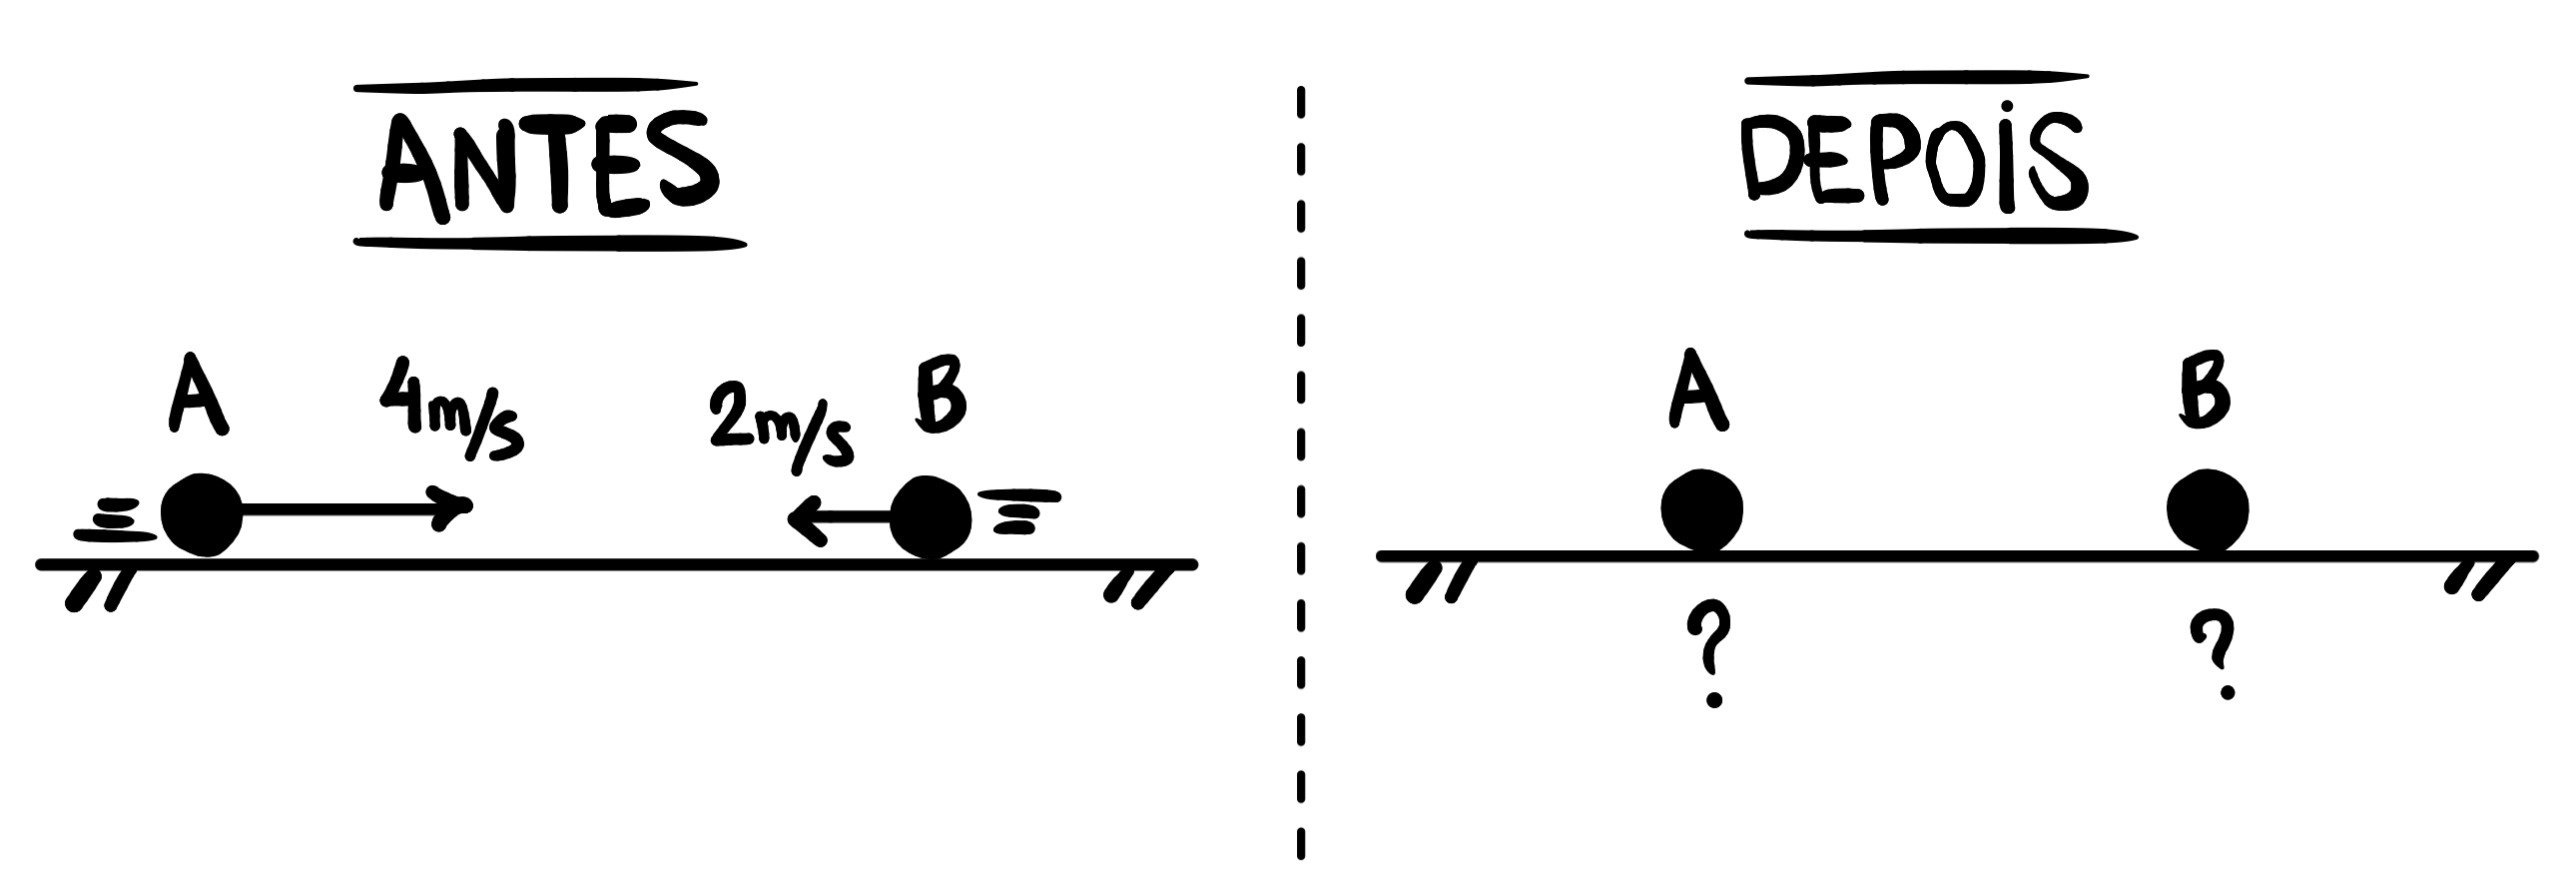
\includegraphics[width=0.7\linewidth]{imagensenergia/colisaoenergia.png}
\captionof{figure}{Colisão elástica entre duas partículas de massas iguais.}
\label{fig_energia_colisaoenergia}
} 
\vspace{0.3cm}

Assumindo que o sentido positivo é para a direita, teremos, da conservação do momento linear:

$$ p_0 = p_f \implies 4m + (-2m) = mv_A + mv_B \implies \boxed{v_A + v_B = 2.}$$

Note, portanto, que é impossível resolver o problema apenas com a conservação do momento linear: tem-se duas incógnitas -- $v_A$ e $v_B$ -- mas apenas uma equação. Se nos for informado, contudo, que trata-se de uma \emph{colisão elástica}, isto é, um tipo específico de colisão no qual a \emph{energia cinética} se conserva, seremos munidos de uma nova equação que nos permitirá relacionar as incógnitas $v_A$ e $v_B$:

$$ E_{\text{C}_0} =  E_{\text{C}_f} \implies \dfrac{1}{2}m4^2 + \dfrac{1}{2}m2^2 = \dfrac{1}{2}mv_A^2 + \dfrac{1}{2}mv_B^2 \implies \boxed{v_A^2 + v_B^2 = 20.}$$

Ora, temos agora duas equações relacionando as incógnitas. Isolando $v_B$ na primeira, temos $v_B = (2 - v_A),$ o que, na segunda, nos leva a

$$ v_A^2 + (2-v_A)^2 = 20, $$

\noindent que, desenvolvendo o produto notável, nos leva a equação do segundo grau $v_A^2 - 2 v_A -8 = 0,$ cujas soluções são $v_A = 4 $ m/s ou $v_A = -2$ m/s. Para cada uma dessas, encontra-se o respectivo valor de $v_B,$ dado por $v_B = (2 - v_A),$ de modo que as soluções são:

$$ v_A = -2 \text{ m/s} \text{ e } v_B = 4 \text{ m/s} \quad \text{ ou } \quad   v_A = 4 \text{ m/s} \text{ e } v_B = -2 \text{ m/s}.$$

A segunda situação representa, na verdade, a situação inicial, de modo que ela é descartada: após o choque certamente as partículas não se moverão com as mesmas velocidades. Sendo assim, após a colisão vemos que a partícula $A$ se moverá com velocidade de 2 m/s para a esquerda -- exatamente a mesma velocidade que a partícula $B$ tinha, antes da colisão -- enquanto que a partícula $B$ se moverá com velocidade de 4 m/s para a direita -- exatamente a mesma velocidade que a partícula $A$ tinha, antes da colisão. Desse modo, as \textbf{partículas -- de mesma massa, ao sofrerem uma colisão elástica -- trocam de vetor velocidade após o choque.} Este é um resultado importante que terá consequências relevantes. O segundo exemplo dessa seção irá explorar uma delas.





\secgfe{Erros comuns}



Um erro bastante comum é confundir os conceitos -- e as proporcionalidades da velocidade -- do momento linear com a energia cinética.

É o erro mais frequente em questões de colisão -- e tem uma ironia histórica por trás. Como já dito, durante cem anos, os próprios físicos cometeram versões desse erro.
 
% \medskip
% \begin{center}
% \begin{tabular}{llll}
% \hline
% \textbf{Grandeza} & \textbf{Fórmula} & \textbf{Tipo} & \textbf{Conserva-se quando\ldots}\\
% \hline
% Momento linear   & $p = mv$                   & Vetor   & Sistema isolado — sempre\\
% Energia cinética & $E_c = \dfrac{mv^2}{2}$    & Escalar & Colisão elástica apenas\\
% \hline
% \end{tabular}
% \end{center}
% \medskip
 
Um exemplo concreto: dois objetos de mesma massa colidem frontalmente com velocidades
iguais e opostas, e grudam. O momento total antes é zero — e permanece zero depois
(os objetos ficam em repouso). A energia cinética antes era
$2 \cdot \frac{mv^2}{2} = mv^2$; depois é zero. Toda ela foi convertida em calor e deformação. Momento conservado; energia cinética não. O aluno que confunde as duas grandezas vai tentar ``conservar'' a errada e obter resultado incorreto.
 
Outro aspecto importante é sobre a proporcionalidade: dobrar a velocidade não faz dobrar a energia cinética.
 
Como $E_c \propto v^2$, dobrar a velocidade \textbf{quadruplica} a energia cinética:
 
\[
    v \;\to\; 2v
    \implies
    E_c' = \frac{m(2v)^2}{2} = 4\cdot\frac{mv^2}{2} = 4E_c.
\]
 
O experimento de Gravesande mostrava isso diretamente na argila: dobrar a velocidade de impacto deixava uma marca quatro vezes mais profunda, não duas vezes. O mesmo vale para freios: um carro a 120\,km/h não precisa do dobro da distância de
frenagem de um carro a 60\,km/h -- precisa de quatro vezes aquela distância.





\secgfe{Observações}




Duas observações são relevantes de serem pontuadas neste momento. A primeira é sobre a unidade de medida da energia cinética, a qual pode ser facilmente desenvolvida:

$$ [E_\text{C}] = \text{kg} \cdot \left( \dfrac{m}{s} \right)^2 = \text{kg} \cdot \text{m}^2/\text{s}^2 = (\text{kg} \cdot \text{m}/\text{s}^2) \cdot \text{m} = [F] \cdot [d] = \text{J (Joule),}$$


\noindent ou seja, como esperado, a energia cinética tem unidade de energia -- a mesma do trabalho --, o Joule (J).

Outra observação é sobre uma forma de escrever a energia cinética em termos do momento linear $p.$ Como dito, as duas grandezas -- momento linear e energia cinética --, apesar de semelhantes, não medem exatamente a mesma coisa. Podemos, inclusive, relacioná-las, partindo da definição de momento:

$$ p = mv \implies v = \dfrac{p}{m},$$

\noindent o que, na definição de energia cinética, implica

$$ E_\text{C} = \dfrac{1}{2} mv^2 = \dfrac{1}{2} \cancel m \dfrac{p^2}{m^\cancel 2} \implies \boxed{E_\text{C} = \dfrac{p^2}{2m}.}$$


Note que, como o momento linear $p$ cresce linearmente com a velocidade $v$, e como a energia cinética cresce quadraticamente com $v,$ isso implica que a energia cinética cresce com o quadrado do momento linear $p,$ como mostra a relação acima.




\vspace{0.3cm}

\begin{exemplo}[Nível I]\label{exemplo_energia_ecineticaex01}

Uma bola de futebol de 450\,g é chutada e atinge velocidade de 72\,km/h.
Qual é sua energia cinética?
 

\resolucao

Convertendo para unidades do SI:
 
\[
    m = 450\,\text{g} = 0{,}450\,\text{kg},
    \qquad
    v = 72\,\frac{\text{km}}{\text{h}} = 20\,\text{m/s}.
\]
 
Aplicando a definição:
 
\[
    E_c = \frac{mv^2}{2}
        = \frac{0{,}450 \cdot 20^2}{2}
        = \frac{0{,}450 \cdot 400}{2}
        = \frac{180}{2}
        = 90\,\text{J}.
\]
 
 
\medskip
Para contextualizar: 90\,J é aproximadamente a energia necessária para erguer uma
laranja (150\,g) até a altura de um prédio de 20 andares (60\,m). Tudo isso armazenado
numa bola de futebol depois de um chute.

\end{exemplo}


\vspace{0.3cm}





\begin{exemplo}[Nível II - Colisões e Energia.] \label{exemplo_energia_ecineticaex02}

Mostre que, em uma colisão elástica -- isto é, uma colisão em que a energia cinética se conserva -- entre duas partículas de massas iguais, as massas trocarão de vetor velocidade após a colisão.

Aplique isso para o pêndulo de Newton: colisão entre sucessivas bolinhas de mesma massa, uma ao lado da outra.

\resolucao

Sejam $v_1$ e $v_2$ as velocidades das duas partículas
(massa $m$ cada) antes da colisão, e $v_1'$ e $v_2'$ após.
As conservações do momento linear e da energia cinética exigem, respectivamente, que

\[
    mv_1 + mv_2 = mv_1' + mv_2'
    \implies
    v_1 + v_2 = v_1' + v_2' \implies \boxed{(v_1 - v_1') = (v_2' - v_2).}
    \tag{I}
\]

\[
    \frac{1}{2}mv_1^2 + \frac{1}{2}mv_2^2
    = \frac{1}{2}mv_1'^2 + \frac{1}{2}mv_2'^2
    \implies
    v_1^2 + v_2^2 = v_1'^2 + v_2'^2,
\]

\noindent em que a última relação pode ser escrita, usando a diferença de quadrados, como


\[
    v_1^2 - v_1'^2 = v_2'^2 - v_2^2
    \implies
    \boxed{(v_1 - v_1')(v_1 + v_1') = (v_2' - v_2)(v_2' + v_2).}
    \tag{II}
\]

\noindent Dividindo (II) por (I), membro a membro:\footnote{O fator $v_1 - v_1' = v_2' - v_2 \neq 0$.}

\[
    v_1 + v_1' = v_2' + v_2
    \tag{III}
\]

\noindent O sistema formado por (I) e (III) é linear:

\[
    \begin{cases}
        v_1 + v_2 = v_1' + v_2'\\[4pt]
        v_1 + v_1' = v_2 + v_2'
    \end{cases}
\]

\noindent Subtraindo a primeira da segunda:

\[
    v_2 - v_1' = v_1' - v_2
    \implies
    \boxed{v_1' = v_2.} 
\]

\noindent Substituindo em (I):

\[
    \boxed{v_2' = v_1.}
\]

\noindent ou seja, as duas partículas \textbf{trocam exatamente suas
velocidades} após a colisão elástica, como queríamos demonstrar.
\medskip
\hline
\medskip
\noindent\textbf{Aplicação ao pêndulo de Newton}

\medskip

No pêndulo de Newton, várias bolinhas idênticas de massa
$m$ estão em contato numa fila, como mostra a Figura \ref{fig_energia_pendulonewton1}.


\vspace{0.3cm}
{
\centering
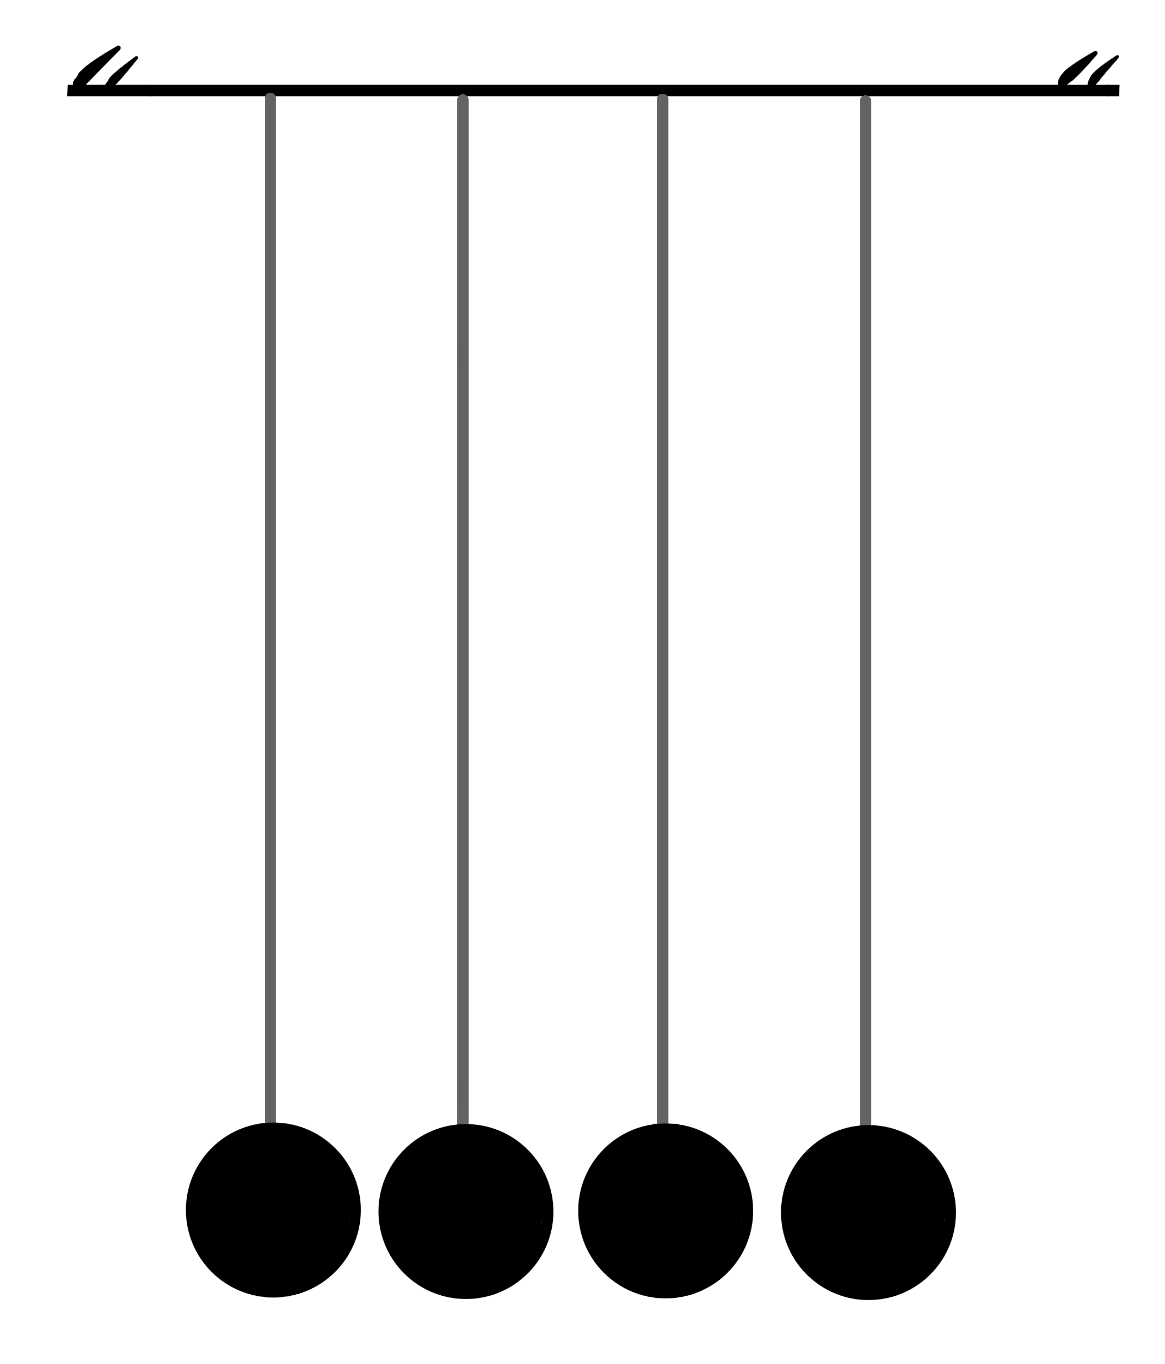
\includegraphics[width=0.25\linewidth]{imagensenergia/pendulonewton1.png}
\captionof{figure}{O pêndulo de Newton.}
\label{fig_energia_pendulonewton1}
} 
\vspace{0.3cm}

Considere a situação em que puxa-se duas bolinhas para a esquerda, abandonando-as, como mostra a Figura \ref{fig_energia_pendulonewton2}. A imagem do meio mostra as duas bolinhas se aproximando, com velocidade $v_0$ cada, das demais bolinhas do sistema, que se encontram paradas. Seria possível, após as colisões, que apenas uma única bolinha saísse do lado direito, com o dobro da velocidade?




\vspace{0.3cm}
{
\centering
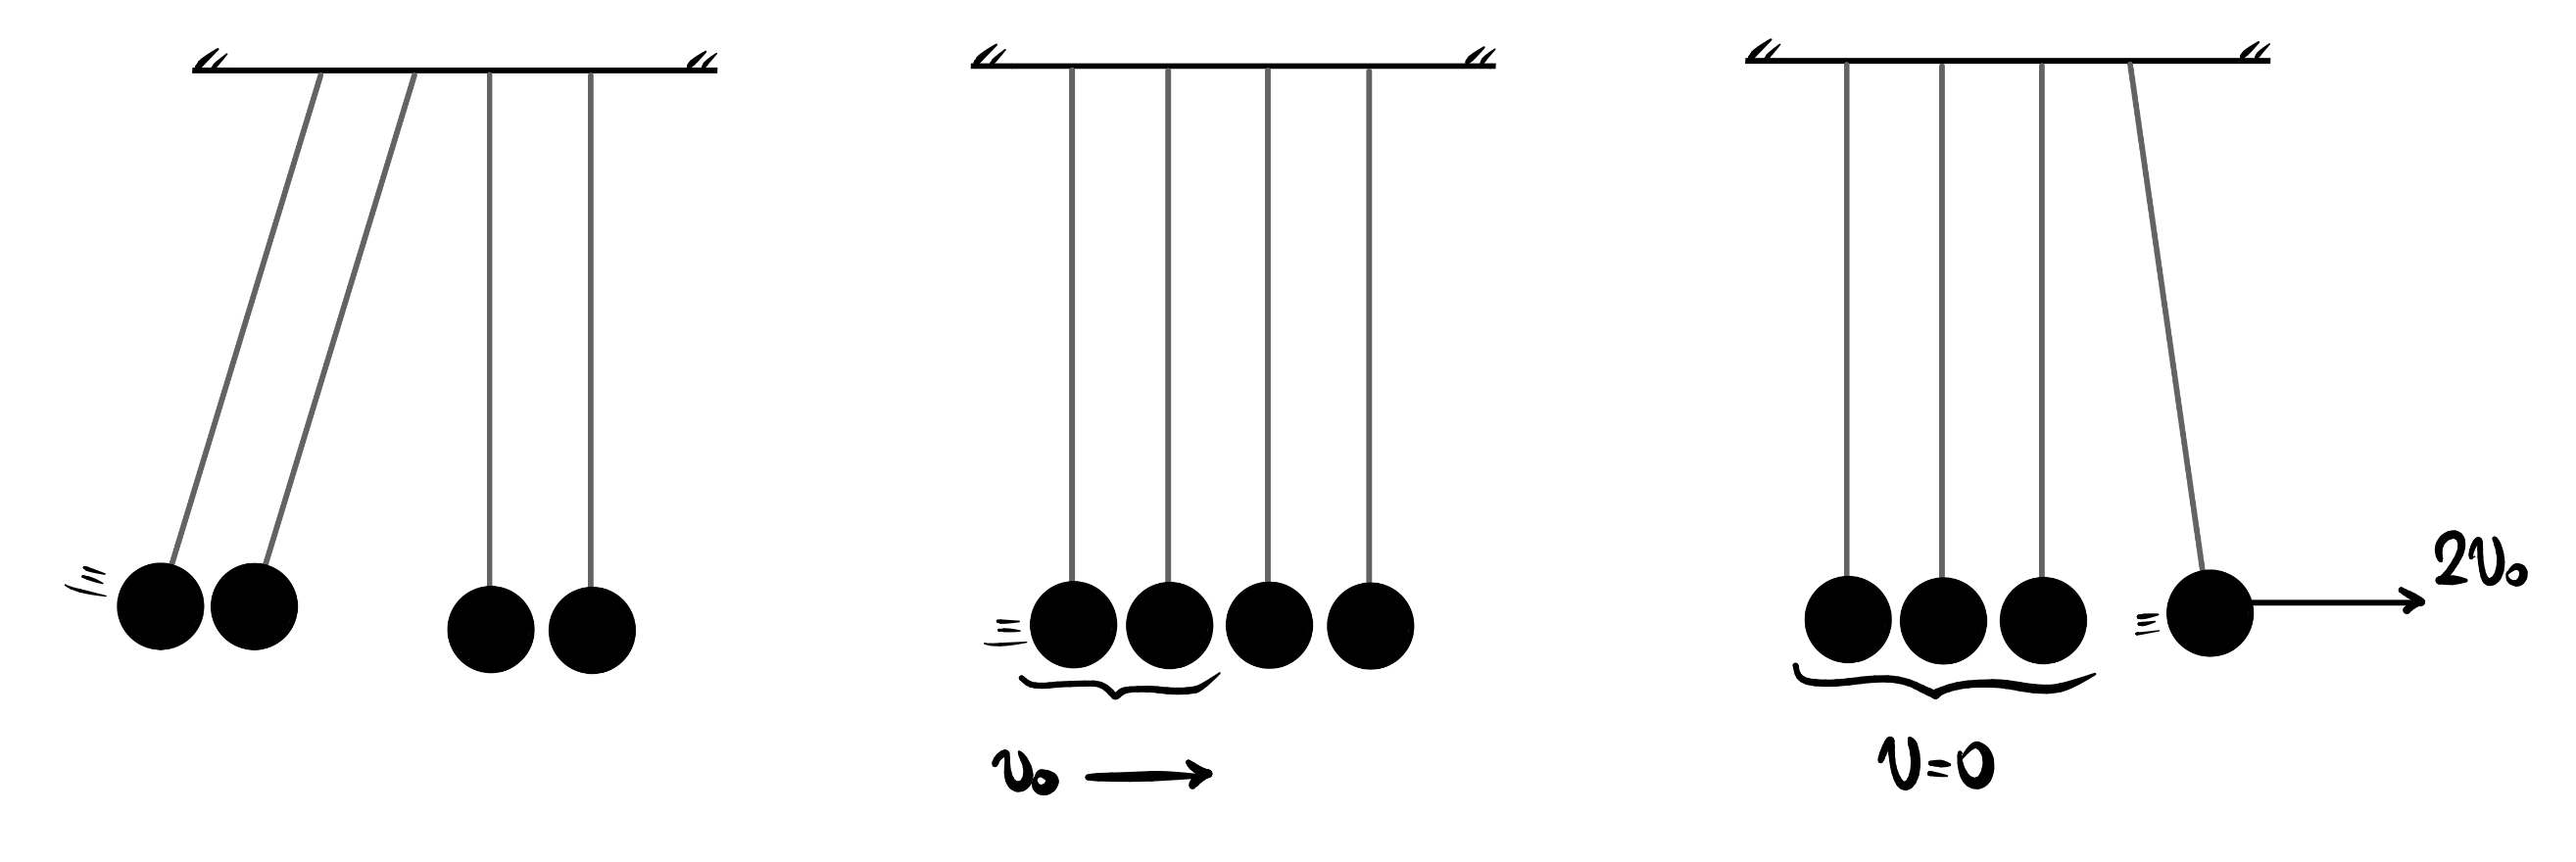
\includegraphics[width=0.8\linewidth]{imagensenergia/pendulonewton2.png}
\captionof{figure}{O pêndulo de Newton: uma situação em que o momento se conserva.}
\label{fig_energia_pendulonewton2}
} 
\vspace{0.3cm}

Ora, essa seria uma configuração em que o momento linear se conservaria, haja vista que 

$$ p_0 = mv_0 + mv_0 = 2mv_0 \quad \text{ e } \quad p_f = m(2v_0) = 2mv_0.$$ 

Logo, a princípio, seria perfeitamente possível com que a situação da Figura \ref{fig_energia_pendulonewton2} ocorresse -- do ponto de vista da lei de conservação do momento linear. Contudo, avaliemos o que ocorre com a energia:

$$ E_{\text{C}_i} = \dfrac{1}{2}mv_0^2 + \dfrac{1}{2}mv_0^2 = mv_0^2 \quad \text{ e } \quad  E_{\text{C}_f} = \dfrac{1}{2}m(2v_0)^2 = 2mv_0^2,$$

\noindent ou seja, a energia cinética do sistema teria dobrado após o choque! Conforme veremos mais adiante -- e tomando emprestado uma citação de Lavoisier -- \emph{na natureza nada se cria, nada se perde, tudo se transforma,} é impossível que se crie energia cinética em um choque como este. No caso, trata-se de um sistema de bolinhas que colidem sem perda de energia,\footnote{Pense no que significa ``perder energia'' numa colisão: ela vai para algum lugar -- calor, som, deformação permanente. O calor exigiria que as moléculas na região de contato ficassem agitadas após o choque; o som exigiria que as bolinhas vibrassem visivelmente; a deformação exigiria que elas saíssem amassadas. Encoste o dedo nas bolinhas após centenas de choques: elas não estão quentes. Ouça: o som da colisão é seco e brevíssimo. Examine a superfície: nenhum amassado. As bolinhas -- normalmente de aço -- são de um material tão rígido que a região de contato se comprime e se recupera em microssegundos, devolvendo ao movimento quase toda a energia que havia armazenado -- exatamente como uma mola perfeita faria. Não é que a energia ``não possa se perder'' por princípio: é que em um sistema como esse ela simplesmente não encontra mecanismo eficiente para escapar.} de modo que a configuração final, para ser fisicamente possível, precisa também satisfazer a conservação da energia mecânica. Note que, na situação em que saíssem duas bolinhas do lado direito, com a mesma velocidade $v_0$ com as outras duas bolinhas chegarão, as duas leis de conservação -- obviamente -- seriam satisfeitas:


$$ p_0 = mv_0 + mv_0 = 2mv_0 \quad \text{ e } \quad p_f =  mv_0 + mv_0 = 2mv_0,$$ 

\noindent e, para a energia cinética, teríamos 

$$ E_{\text{C}_i} = \dfrac{1}{2}mv_0^2 + \dfrac{1}{2}mv_0^2 = mv_0^2 \quad \text{ e } \quad  E_{\text{C}_f} =  \dfrac{1}{2}mv_0^2 + \dfrac{1}{2}mv_0^2 = mv_0^2,$$

\noindent ou seja, a energia também se conservaria. \\

Este é um belo resultado: ao puxar $3$ bolinhas de um lado, após as colisões, sairão exatamente 3 bolinhas do outro lado, com a mesma velocidade. Por mais que a configuração em que saísse apenas uma bolinha com o triplo da velocidade respeitasse a conservação do momento linear ($p_0= 3mv_0 = m(3v_0) = p_f$), isso violaria a conservação da energia cinética: teríamos criado energia cinética. O jeito de respeitar os dois princípios é saindo, do outro lado, exatamente o mesmo número de bolinhas, com exatamente a mesma velocidade.\\

Concentrar o momento de três partículas em apenas uma cria energia. Isso não é coincidência — é uma
consequência direta de $v^2$ crescer mais rápido que $v$. Se
você concentra as três velocidades $v_0$ de cada partícula da esquerda em uma única partícula, que sairá pela direita com velocidade $3v_0$, o momento se conserva linearmente -- mas a energia aumenta pelo fator $3$, porque o quadrado de $3v_0$ é nove vezes
maior que o quadrado de $v_0$, e dividir a massa por 3 (temos apenas uma partícula saindo do lado direito, e não três) só ameniza um terço deste aumento.

\medskip
Generalizando: considere a situação da Figura \ref{fig_energia_pendulonewton3}, em que puxamos $n$ bolinhas do lado esquerdo, que chegam para colidir, digamos, com uma velocidade $v_0$ com as demais. Suponha que saíam, do lado direito, $m$ bolinhas, todas com uma certa velocidade $v_f,$ após todos os choques. Cada bolinha tem massa $M$\footnote{Atenção: não confundir $M,$ que é a massa de cada bolinha, com $m$, que o número de bolinhas que se movem para a direita após o choque.}.

\vspace{0.3cm}
{
\centering
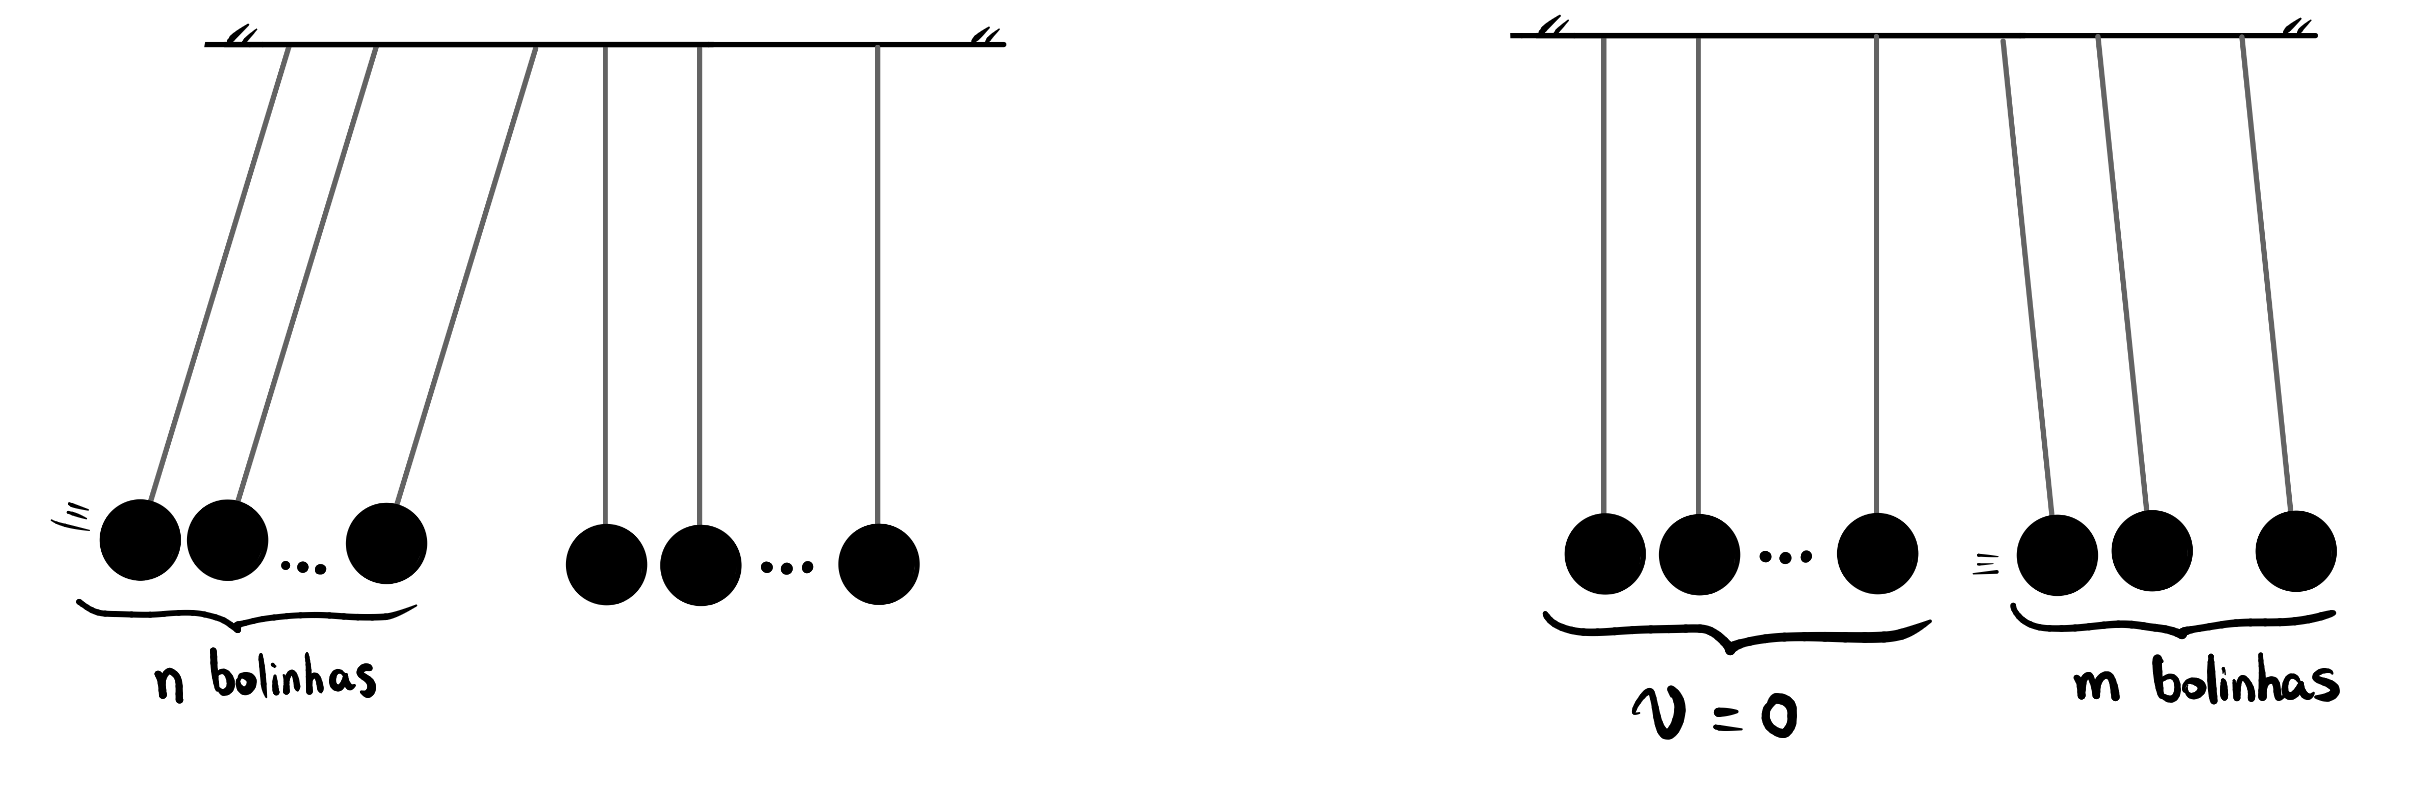
\includegraphics[width=0.8\linewidth]{imagensenergia/pendulonewton3.png}
\captionof{figure}{O pêndulo de Newton: caso geral.}
\label{fig_energia_pendulonewton3}
} 
\vspace{0.3cm}

O momento linear total inicial é $p_0 = n \cdot(Mv_0)$ e o momento linear total final é $p_f = m(Mv_f)$. A lei da conservação do momento exige que

$$ p_0 = p_f \implies n \cdot(\cancel Mv_0) = m(\cancel Mv_f) \implies \boxed{n v_0 = m v_f.} $$

A conservação da energia cinética exige que

$$  E_{\text{C}_i} =   E_{\text{C}_f} \implies n \cdot\dfrac{1}{2} M v_0^2 = m \cdot\dfrac{1}{2} M v_f^2 \implies \boxed{nv_0^2 = mv_f^2.} $$

Dividindo as duas relações acima, membro a membro, teremos

$$ \dfrac{nv_0^2}{n v_0} = \dfrac{mv_f^2}{m v_f} \implies  \boxed {v_0 = v_f,}$$

\noindent ou seja, a velocidade de cada uma das $m$ bolinhas que saem do lado direito deve ser exatamente igual à velocidade das $n$ bolinhas que chegaram do lado esquerdo. Além disso, substituindo tal resultado em qualquer uma das duas relações que o originaram, produz:

$$ n \cancel{v_0} = m \cancel{v_f} \implies \boxed{n=m,}$$

\noindent ou seja, a quantidade de bolinhas que saem do lado direito é exatamente igual à quantidade de bolinhas que chegaram pelo lado esquerdo. Há de ser assim para que se respeitem os dois princípios de conservação: da energia e do momento linear. É por isso que a situação da Figura \ref{fig_energia_pendulonewton2} não é fisicamente possível: ela só respeita um desses princípios -- o da conservação do momento linear. Naquela situação, ao puxar duas bolinhas de um lado, teriam que sair exatamente duas do outro, com a mesma velocidade. Assim é o funcionamento do pêndulo de Newton.

\end{exemplo}


\vspace{0.3cm}





\begin{exemplo}[Nível III]\label{exemplo_energia_ecineticaex03}

Uma bala de massa $m$ é disparada horizontalmente com velocidade
$v_0$ contra um bloco $B,$ de massa $3m$, em repouso sobre uma
superfície horizontal sem atrito. A bala se aloja no bloco $B$.
O conjunto (bala\,+\,$B$) desliza e colide elasticamente com um
terceiro bloco $C$, de massa $2m$, também em repouso.

\begin{enumerate}
    \item [a)]Determine a velocidade $V$ do conjunto (bala\,+\,$B$)
    imediatamente após a primeira colisão, e a fração da energia
    cinética inicial da bala que foi dissipada.

    \item [b)] Determine as velocidades do conjunto (bala\,+\,$B$) e
    do bloco $C$ após a colisão elástica.


\end{enumerate}

\resolucao

\noindent\textit{a)} Pela conservação do momento linear na primeira colisão, teremos:

\[
    mv_0 = (m + 3m)V = 4mV
    \implies
    \boxed{V = \frac{v_0}{4}}
\]

\noindent A fração da energia cinética inicial dissipada na colisão:

\[
    \frac{\Delta E}{E_0}
    = \frac{\dfrac{1}{2}mv_0^2 - \dfrac{1}{2}(4m)V^2}{\dfrac{1}{2}mv_0^2}
    = 1 - \frac{4m \cdot v_0^2/16}{mv_0^2}
    = 1 - \frac{1}{4}
    = \boxed{\frac{3}{4} = 75\%.}
\]


\medskip
\noindent\textit{b)} O conjunto (bala\,+\,$B$), de massa $4m$, move-se com
velocidade $V = v_0/4$ e colide com o bloco $C$ (massa $2m$, em
repouso). Chamemos de $v_{AB}'$ e $v_C'$ as velocidades após
a colisão. As duas leis de conservação fornecem:

\medskip
\noindent\textbf{Conservação do momento linear:}

\[
    4m\cdot\frac{v_0}{4} + 2m\cdot 0
    = 4m\,v_{AB}' + 2m\,v_C'
\]

\[
    mv_0 = 4m\,v_{AB}' + 2m\,v_C'
    \implies
    v_0 = 4\,v_{AB}' + 2\,v_C'
    \tag{I}
\]

\noindent\textbf{Conservação da energia cinética:}

\[
    \frac{1}{2}(4m)\left(\frac{v_0}{4}\right)^{\!2}
    =
    \frac{1}{2}(4m)\,v_{AB}'^{\,2} + \frac{1}{2}(2m)\,v_C'^{\,2}
\]

\[
    \frac{mv_0^2}{8}
    = 2m\,v_{AB}'^{\,2} + m\,v_C'^{\,2}
    \implies
    \frac{v_0^2}{8} = 2\,v_{AB}'^{\,2} + v_C'^{\,2}
    \tag{II}
\]


\medskip
\noindent De (I): $v_C' = \dfrac{v_0 - 4\,v_{AB}'}{2}$.
Substituindo em (II):

\[
    \frac{v_0^2}{8}
    = 2\,v_{AB}'^{\,2}
    + \left(\frac{v_0 - 4\,v_{AB}'}{2}\right)^{\!2}
    = 2\,v_{AB}'^{\,2}
    + \frac{v_0^2 - 8\,v_0\,v_{AB}' + 16\,v_{AB}'^{\,2}}{4}
\]

\noindent Multiplicando tudo por 8 e manipulando, somos levados a 

\[
  48\,v_{AB}'^{\,2} - 16\,v_0\,v_{AB}' + v_0^2 =0,
\]

\noindent em que as duas raízes são:

\[
    v_{AB}' = \frac{24v_0}{96} = \frac{v_0}{4}
    \qquad\text{ou}\qquad
    v_{AB}' = \frac{8v_0}{96} = \frac{v_0}{12}
\]

\noindent A raiz $v_{AB}' = v_0/4$ corresponde à situação
\textit{antes} da colisão — o sistema não interagiu — e deve
ser descartada. A solução física é:

\[
    \boxed{v_{AB}' = \frac{v_0}{12}}.
\]

\noindent E, voltando a (I):

\[
    v_C' = \frac{v_0 - 4\cdot\dfrac{v_0}{12}}{2}
         = \frac{v_0 - \dfrac{v_0}{3}}{2}
         = \frac{\dfrac{2v_0}{3}}{2}
         = \boxed{\frac{v_0}{3}.}
\]

\medskip
\noindent\textbf{Verificação das quantidades conservadas:}

\[
    p_f = 4m\cdot\frac{v_0}{12} + 2m\cdot\frac{v_0}{3}
        = \frac{mv_0}{3} + \frac{2mv_0}{3} = mv_0 = p_i
    \quad\checkmark
\]

\[
    E_f = \frac{1}{2}(4m)\!\left(\frac{v_0}{12}\right)^{\!2}
        + \frac{1}{2}(2m)\!\left(\frac{v_0}{3}\right)^{\!2}
        = \frac{mv_0^2}{72} + \frac{mv_0^2}{9}
        = \frac{mv_0^2}{8} = E_i
    \quad\checkmark
\]

\medskip
O surgimento de duas raízes na resolução da equação quadrática
é esperado: sempre que se resolve um sistema com uma equação
linear (momento) e uma quadrática (energia), obtém-se duas
soluções. Uma delas é sempre a situação trivial
``antes da colisão'' — matematicamente válida, mas fisicamente
descartável. A solução física é sempre a outra raiz.
Este é um padrão que o leitor encontrará repetidamente em
problemas de colisão elástica.



\end{exemplo}


\vspace{0.3cm}
















\begin{secnivel}[Teorema da Energia Cinética]{I}{Teorema da Energia Cinética}
 

  \eqLdois{dem}{eq_energia_teoremaenergiacinetica}{W = \Delta E_\text{C}}
  
\end{secnivel}







\secgfe{De onde vem}

A Equação \eqref{eq_energia_teoremaenergiacinetica} diz que o trabalho de uma força é a forma pela qual se injeta (ou se retira) energia cinética de um sistema. O trabalho da força resultante $W$ é, justamente, igual à variação da energia cinética sofrida pela partícula.

Vamos verificar isso para o caso de um movimento já conhecido por nós -- o Movimento Uniformemente Variado. Considere, por exemplo, a situação da Figura \ref{fig_mec_torricelli02} (p. \pageref{fig_mec_torricelli02}), que mostra um carro com velocidade inicial $v_0$ sendo empurrado por uma força constante $F.$ Tal força imprimirá no carro uma aceleração dada por $a=F/m$, o que aumentará sua velocidade até o valor $v$ após um deslocamento $d$.

Ora, já é imediato notar que a aplicação de uma força ao longo de um deslocamento -- a realização de um trabalho por essa força -- alterou a energia cinética da partícula, haja vista que sua velocidade aumentou. Podemos relacionar essas grandezas cinemáticas por meio da Equação de Torricelli:

$$ v^2 = v_0^2 + 2ad,$$

\noindent que, multiplicando ambos os lados pela massa $m$ da partícula, nos leva a

$$ mv^2 = mv_0^2 + 2\cdot \underbrace{ma}_{F_R} \cdot d,$$

\noindent e, dividindo ambos os lados por 2, teremos:

$$ \dfrac{mv^2}{2} = \dfrac{mv_0^2}{2} + F\cdot d, $$

\noindent ou seja, vemos que o trabalho foi o responsável por variar a energia cinética do sistema:

$$ W = F \cdot d = \dfrac{mv^2}{2} - \dfrac{mv_0^2}{2} = \Delta E_c, $$

\noindent como atesta a Equação \eqref{eq_energia_teoremaenergiacinetica}.


Nós provamos a validade da Equação \eqref{eq_energia_teoremaenergiacinetica} para o caso de um Movimento Uniformemente Variado, por ser uma situação conhecida pelo leitor. Tal equação, contudo, vale de forma geral, para absolutamente qualquer tipo de movimento. Ela atesta, portanto, um princípio geral: o trabalho é o meio pelo qual consegue-se, através de uma força, injetar ou retirar energia cinética de um sistema. Em outros volumes estudaremos diferentes processos de transferência de energia nos quais o trabalho, novamente, estará presente.

Demonstrar a validade de tal equação para o caso geral, em que ela valha para absolutamente qualquer tipo de movimento, é tarefa que exige conhecimentos matemáticos mais avançados, como o uso do Cálculo Integral e Diferencial. Para não dizer que o leitor há de se contentar com o que tem, há uma breve digressão de forma simplificada sobre como podemos provar isso para o caso geral no Apêndice \ref{apendice-teoremaenergiacinetica}.

\secgfe{Onde é usada}

Este teorema pode ser usado diretamente para resolver problemas de dinâmica, como veremos em alguns exemplos. Contudo, este não é o motivo pelo qual enunciamos e estudamos tal teorema, haja vista que esses problemas que serão resolvidos por ele também poderiam, sem dificuldade, serem resolvidos usando apenas as leis de Newton. Deixaremos isso claro nos exemplos resolvidos.

O real motivo de enunciarmos o teorema dado pela Equação \eqref{eq_energia_teoremaenergiacinetica} é porque ele será um passo intermediário para construir o teorema mais importante dessa seção -- e, este sim, terá uma extensão de aplicabilidade que superará o que pode ser feito apenas com as leis de Newton, como veremos mais adiante. Trata-se do Princípio da Conservação da Energia, enunciado pela Equação \eqref{eq_energia_conservacaodaenergiamecanica}.



\secgfe{Erros comuns}

Vale pontuar alguns erros simples que costumam ser recorrentes entre os principiantes neste conteúdo:

\begin{enumerate}
    \item [(i)] Um estudante analisa um bloco sendo puxado por uma corda com força $F$ enquanto o
atrito age na direção oposta. Ele aplica o Teorema da Energia Cinética usando apenas o
trabalho da força $F$, ignorando o atrito, e obtém uma velocidade final maior do que a real.

O equívoco está em confundir o trabalho de \emph{uma} força com o trabalho da
\emph{resultante}. O teorema é preciso: $W = \Delta E_c$, em que $W$ é o
trabalho realizado pela \emph{soma vetorial} de todas as forças -- a força resultante que atua sobre a partícula.\footnote{Na verdade, é possível sempre tomar dois caminhos: achar a resultante das forças $\vec F_R$ e calcular o seu trabalho, que seria o trabalho total $W$ feito sobre a partícula. Ou, então, pode-se calcular o trabalho feito por cada força individual e, depois, somar algebricamente todos eles, o que dará o mesmo resultado: o trabalho total $W$ feito sobre a partícula.} Ao ignorar o atrito, o
estudante calculou $W_\text{F}$, o trabalho realizado apenas pela força $F$, e não $W$, o trabalho total, realizado pela resultante das forças. O correto seria:
%
\begin{equation*}
    W = W_\text{F} + W_\text{FAT},
\end{equation*}
%

Somente após somar todos os trabalhos é que o teorema pode ser aplicado.


    \item [(ii)] Em um problema onde um objeto desce um plano inclinado sem atrito, o estudante
calcula $W = F_\text{R} \cdot d$, usando $d$ como o comprimento do plano, mas
substitui $F_\text{R} = mg$ (o peso total), sem decompor.

O erro é aplicar a força \emph{total} em uma direção diferente do deslocamento. O peso age
verticalmente, mas o deslocamento é ao longo do plano. O trabalho de uma força é
$W = F \cdot d \cdot \cos\theta$, onde $\theta$ é o ângulo entre a força e o
deslocamento. No plano inclinado de ângulo $\alpha$, o trabalho do peso é:
%
\begin{equation*}
    W_\text{P} = mg \cdot d \cdot \sin\,\alpha,
\end{equation*}
%

O trabalho da força normal é nulo, pois ela é perpendicular ao movimento em todos os pontos da trajetória.
\end{enumerate}




\secgfe{Observações}

Como o trabalho envolve o produto da força pelo deslocamento da partícula ao longo da direção da força, já havíamos pontuado que forças centrípetas -- perpendiculares à direção de deslocamento e, portanto, com componente nula na direção do deslocamento -- não realizam trabalho. Agora, a Equação \eqref{eq_energia_teoremaenergiacinetica} nos permite compreender por qual razão, sob a ação exclusivamente de uma força desse tipo, a partícula deve se mover com velocidade constante.



\vspace{0.3cm}
{
\centering
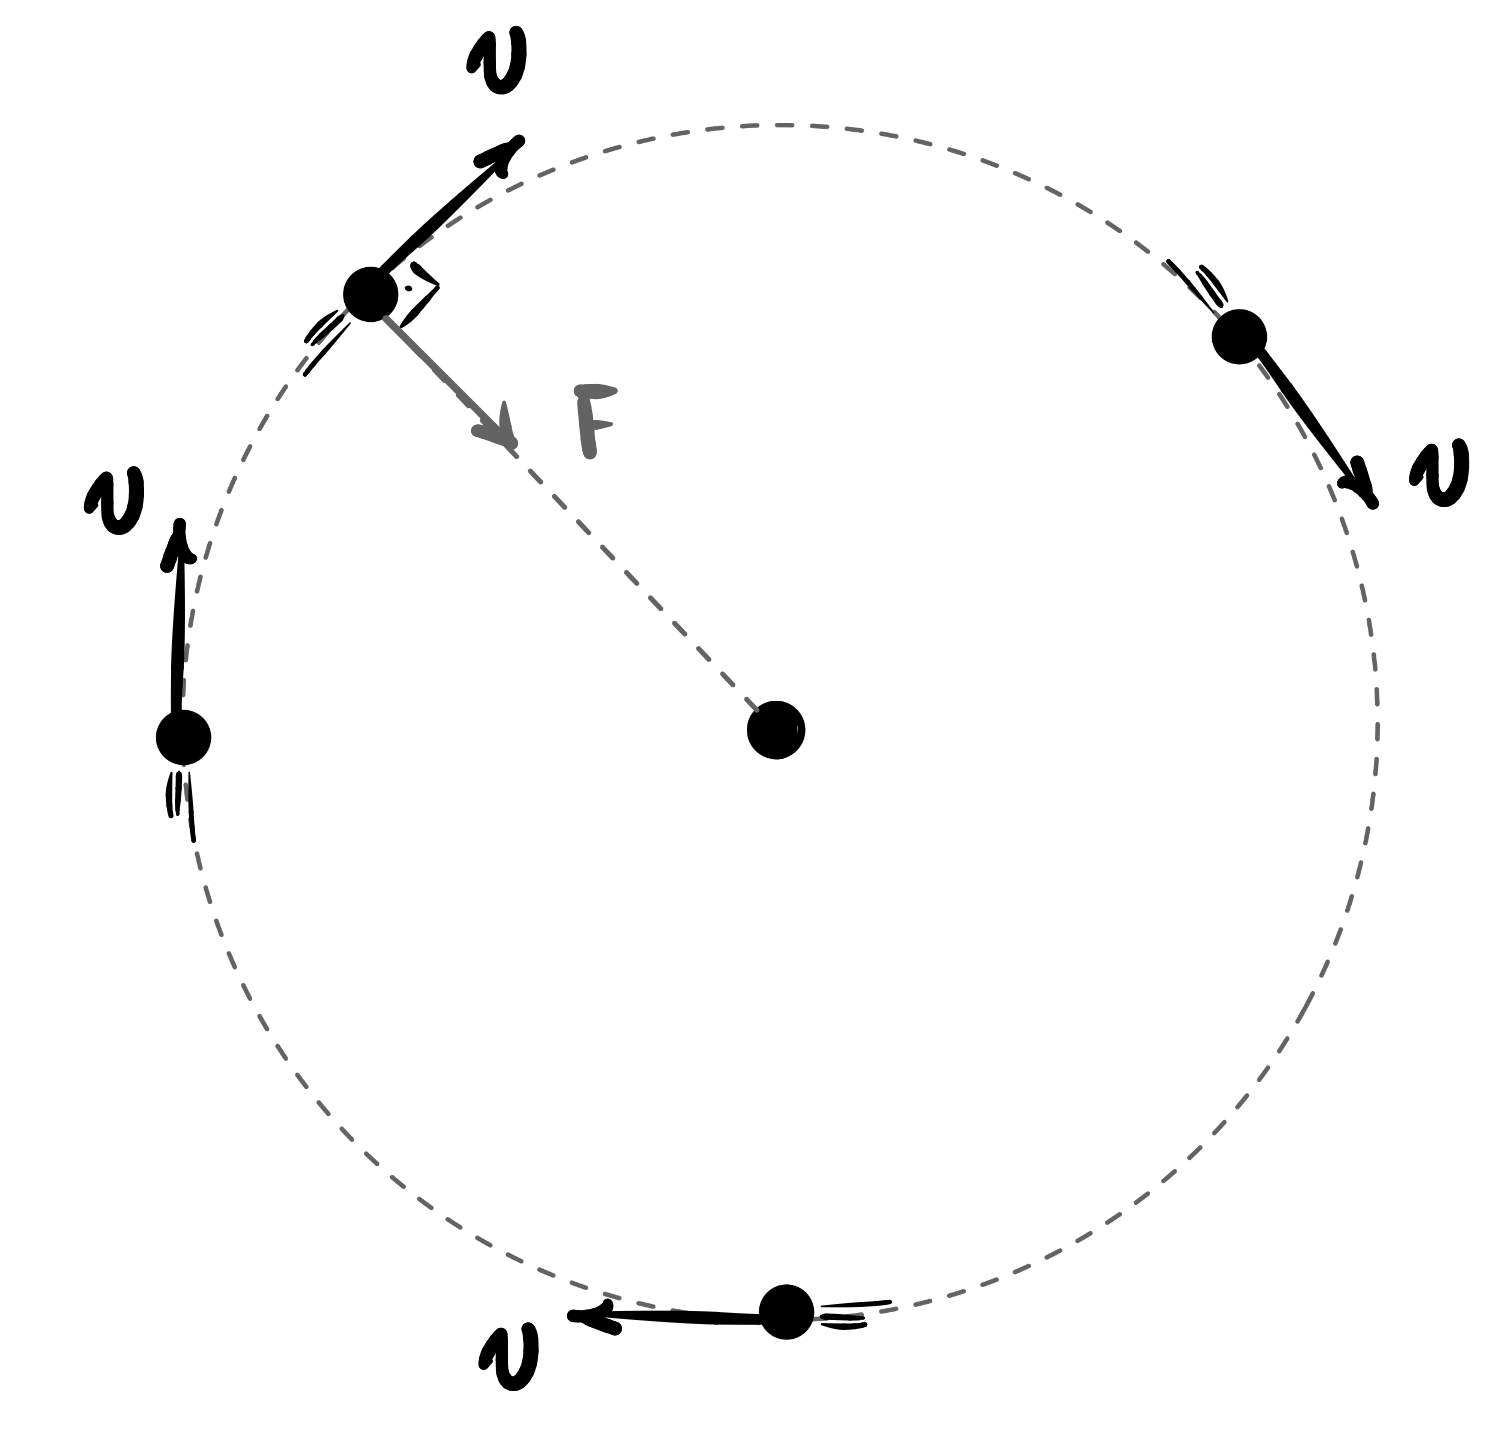
\includegraphics[width=0.35\linewidth]{imagensenergia/teoremaenergiacineticacentripeta.png}
\captionof{figure}{Forças centrípetas não alteram a energia cinética da partícula, haja vista que não realizam trabalho.}
\label{fig_energia_teoremaenergiacineticacentripeta}
} 
\vspace{0.3cm}

Sendo o trabalho o agente responsável por variar a energia cinética de uma partícula, se o trabalho de uma certa força é nulo, a energia cinética -- e, portanto, a velocidade -- de tal partícula deve ficar inalterada. 

Nós já sabíamos que as forças que apontam para o centro geram a aceleração centrípeta, e que esta é responsável unicamente por variar a direção do vetor velocidade, deixando seu módulo inalterado. O que muda aqui é a forma, a linguagem como se explica este mesmo fato, já conhecido por nós.




\vspace{0.3cm}

\begin{exemplo}[Nível I]\label{exemplo_energia_teoremaenergiacinetica01}

Um carrinho de supermercado de massa $15\,\text{kg}$ está em repouso.
Uma criança empurra o carrinho com uma força horizontal constante de
$30\,\text{N}$ por uma distância de $2\,\text{m}$ ao longo de um corredor
liso (sem atrito). Qual é a velocidade do carrinho ao final do percurso?

\resolucao

Como já discutimos, os conceitos de trabalho e energia cinética constituem apenas uma nova linguagem para descrever a dinâmica, isto é, explicar porque os corpos se movem como se movem. Sendo assim, em diversos problemas deste tema o leitor terá, muitas vezes, dois caminhos possíveis: resolver usando a linguagem vetorial, da forças e acelerações (leis de Newton), ou resolver usando a linguagem escalar, de trabalho e energia. Façamos das duas formas para deixar isso claro ao leitor.
\bigskip

\textbf{Solução 01: Leis de Newton} \\

Como não há atrito e a força aplicada é horizontal, ela é a única força na
direção do movimento. Pela Segunda Lei de Newton:
%
\begin{equation*}
    F = ma \implies a = \frac{F}{m} = \frac{30}{15} = 2\,\text{m/s}^2.
\end{equation*}
%
O carrinho parte do repouso ($v_0 = 0$). Usando a equação de Torricelli:
%
\begin{equation*}
    v^2 = v_0^2 + 2a\Delta s = 0 + 2 \cdot 2 \cdot 2 = 8\,\text{m}^2/\text{s}^2
    \implies \boxed{v = 2\sqrt{2} \text{ m/s}.}
\end{equation*}

\bigskip
\textbf{Solução 02: Trabalho e Energia} \\

O trabalho realizado pela força resultante (única força horizontal) é:
%
\begin{equation*}
    W = F \cdot \Delta s = 30 \cdot 2 = 60\,\text{J}.
\end{equation*}
%
Pelo Teorema da Energia Cinética, com $v_0 = 0$:
%
\begin{equation*}
    W = \frac{1}{2}mv^2 - \frac{1}{2}mv_0^2
    \implies 60 = \frac{1}{2} \cdot 15 \cdot v^2
    \implies v^2 = 8\,\text{m}^2/\text{s}^2
    \implies \boxed{v = 2\sqrt{2} \text{ m/s}.}
\end{equation*}
%
Ambos os caminhos chegam ao mesmo resultado --- como deve ser. O método
da energia, contudo, dispensa o cálculo explícito da aceleração, o que o
torna especialmente eficiente quando as forças envolvidas são oblíquas ou
variáveis, como veremos mais adiante.


\end{exemplo}


\vspace{0.3cm}





\begin{exemplo}[Nível II]\label{exemplo_energia_teoremaenergiacinetica02}

Uma bala de $10\,\text{g}$ viaja a $400\,\text{m/s}$ e penetra em uma placa
de madeira, saindo pelo outro lado com velocidade de $100\,\text{m/s}$.
Sabendo que a espessura da placa é de $5\,\text{cm}$, determine a força
média de resistência exercida pela madeira sobre a bala.


\resolucao

Façamos a solução pelos dois caminhos conhecidos como no exemplo anterior.

\bigskip

\textbf{Solução 01: Leis de Newton} \\

Convertemos as grandezas para o SI\@: $m = 0{,}010\,\text{kg}$,
$v_0 = 400\,\text{m/s}$, $v = 100\,\text{m/s}$, $\Delta s = 0{,}05\,\text{m}$.

A aceleração (negativa, pois a força é contrária ao movimento) é obtida
pela equação de Torricelli:
%
\begin{equation*}
    v^2 = v_0^2 + 2a\Delta s
    \implies a = \frac{v^2 - v_0^2}{2\,\Delta s}
    = \frac{(100)^2 - (400)^2}{2 \cdot 0{,}05}
    = -1\,500\,000\,\text{m/s}^2.
\end{equation*}
%
Pela Segunda Lei de Newton:
%
\begin{equation*}
    F_\text{R} = m\,a = 0{,}010 \cdot (-1\,500\,000)
    = \boxed{-15\,000\,\text{N} = -15\,\text{kN},}
\end{equation*}

\noindent em que o sinal negativo indica que a força aponta no sentido contrário ao da velocidade inicial $v_0,$ como esperado.



\bigskip
\textbf{Solução 02: Trabalho e Energia} \\

O trabalho realizado pela força de resistência (oposta ao movimento) é, pelo Teorema da Energia Cinética:
%
\begin{align*}
    W &= \frac{1}{2}mv^2 - \frac{1}{2}mv_0^2 \\[4pt]
               &= \frac{1}{2}(0{,}010)(100)^2
                  - \frac{1}{2}(0{,}010)(400)^2 \\[4pt]
               &= 50 - 800 = -750\,\text{J}.
\end{align*}
%
Da definição de trabalho, $W = F_\text{R}\cdot\Delta s$, teremos:
%
\begin{equation*}
    -750 = F_\text{R} \cdot 0{,}05
    \implies \boxed{F_\text{R} = -15\,000\,\text{N} = -15\,\text{kN}.}
\end{equation*}
%
Esse resultado ilustra com clareza por que materiais densos são eficazes
como blindagem: em deslocamentos muito pequenos, forças enormes são geradas
para absorver a energia cinética do projétil. Note que o resultado final foi o mesmo pelos dois caminhos, como esperado.


\end{exemplo}


\vspace{0.3cm}





\begin{exemplo}[Nível III]\label{exemplo_energia_teoremaenergiacinetica03}

Um bloco de massa $m$ desliza sobre uma superfície horizontal cujo
coeficiente de atrito cinético \emph{não é constante}, mas varia com a
posição segundo a lei
%
\begin{equation*}
    \mu(x) = \mu_0\!\left(1 + \frac{x}{L}\right),
\end{equation*}
%
onde $\mu_0$ e $L$ são constantes conhecidas. O bloco parte de $x = 0$
com velocidade $v_0$. Determine a velocidade do bloco em $x = L$ e a
condição sobre $v_0$ para que ele de fato alcance essa posição.

\resolucao

O primeiro passo é escrever a força de atrito em função da posição.
Como a superfície é horizontal, a normal é $N = mg$ em todo ponto, e
portanto, a força de atrito $f(x)$ em cada posição $x$ será dada por
%
\begin{equation*}
    f(x) = \mu N = \mu(x)\,mg = \mu_0 mg\!\left(1 + \frac{x}{L}\right).
\end{equation*}
%
Trata-se de uma função \emph{linear} de $x$: em $x = 0$ vale
$f(0) = \mu_0 mg$, e em $x = L$ vale $f(L) = 2\mu_0 mg$. O gráfico
$f \times x$ é, portanto, um segmento de reta que sobe de
$\mu_0 mg$ até $2\mu_0 mg$ ao longo do intervalo $[0, L]$, como
ilustrado abaixo.

\bigskip

% --- Gráfico f(x) ---
\begin{center}
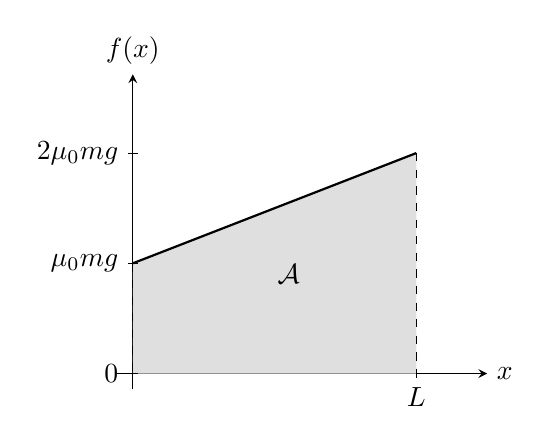
\begin{tikzpicture}[>=stealth, scale=1.0]

  % Eixos
  \draw[->] (-0.2, 0) -- (4.5, 0) node[right] {$x$};
  \draw[->] (0, -0.2) -- (0, 3.8) node[above] {$f(x)$};

  % Coordenadas do trapézio
  % x=0  -> y = mu0*mg  (representado por 1.4)
  % x=L  -> y = 2*mu0*mg (representado por 2.8)
  % L representado por 3.6

  \def\xL{3.6}
  \def\yA{1.4}   % f(0) = mu0*mg
  \def\yB{2.8}   % f(L) = 2*mu0*mg

  % Área hachurada (trapézio)
  \fill[gray!25] (0,0) -- (0,\yA) -- (\xL,\yB) -- (\xL,0) -- cycle;

  % Linha da força
  \draw[thick] (0,\yA) -- (\xL,\yB);

  % Lados do trapézio
  \draw[dashed] (0,\yA)   -- (0,0);
  \draw[dashed] (\xL,\yB) -- (\xL,0);

  % Marcas no eixo x
  \draw (\xL, 0.06) -- (\xL, -0.06) node[below] {$L$};
  \draw (0.06, 0)   -- (-0.06, 0)   node[left]  {$0$};

  % Marcas no eixo y
  \draw (0.06, \yA) -- (-0.06, \yA) node[left] {$\mu_0 mg$};
  \draw (0.06, \yB) -- (-0.06, \yB) node[left] {$2\mu_0 mg$};

  % Rótulo da área
  \node at ({0.55*\xL}, {0.45*\yB}) {$\mathcal{A}$};

\end{tikzpicture}
\end{center}

\bigskip

\noindent O trabalho de uma força variável é a área sob a curva
$f \times x$. No caso do atrito, a força é
sempre oposta ao deslocamento, de modo que seu trabalho é o
\emph{negativo} dessa área.

A região hachurada no gráfico é um \textit{trapézio} de bases paralelas
$f(0) = \mu_0 mg$ e $f(L) = 2\mu_0 mg$, e altura (na direção de $x$)
igual a $L$. Sua área é:
%
\begin{equation*}
    \mathcal{A} = \frac{f(0) + f(L)}{2}\cdot L
    = \frac{\mu_0 mg + 2\mu_0 mg}{2}\cdot L
    = \frac{3\mu_0 mg}{2}\cdot L.
\end{equation*}
%
Portanto, o trabalho do atrito ao longo de $[0,\, L]$ é:
%
\begin{equation*}
    W_\text{FAT} = -\mathcal{A} = -\frac{3\mu_0 mgL}{2}.
\end{equation*}
%
Nenhuma outra força realiza trabalho: a normal e o peso são
perpendiculares ao movimento. Logo, o trabalho total é $W = W_\text{FAT} $.

Pelo Teorema da Energia Cinética:
%
\begin{equation*}
    W = \frac{1}{2}mv^2 - \frac{1}{2}mv_0^2
    \implies
    -\frac{3\mu_0 mgL}{2} = \frac{1}{2}mv^2 - \frac{1}{2}mv_0^2.
\end{equation*}
%
Dividindo tudo por $\tfrac{1}{2}m$ e isolando $v^2$:
%
\begin{equation*}
    v^2 = v_0^2 - 3\mu_0 gL
    \implies
    \boxed{v = \sqrt{v_0^2 - 3\mu_0 gL}.}
\end{equation*}
%
Para que o bloco de fato alcance $x = L$ com velocidade real,
é necessário que $v^2 \geq 0$:
%
\begin{equation*}
    \boxed{v_0 \;\geq\; \sqrt{3\mu_0 gL}.}
\end{equation*}
%
Se $v_0 = \sqrt{3\mu_0 gL}$, o bloco chega exatamente parado em
$x = L$. Se $v_0 < \sqrt{3\mu_0 gL}$, ele para antes desse ponto.
\bigskip

Dois resultados merecem atenção. Primeiro, a massa $m$ cancelou-se
inteiramente na expressão de $v$ --- assim como na queda livre, isso
não é coincidência: tanto o atrito quanto a inércia escalam com $m$,
de modo que a dinâmica é a mesma para qualquer massa. 
\bigskip

Segundo, e mais sutil: a velocidade em $x = L$ não depende de \emph{como} o coeficiente
varia ao longo do trajeto, mas apenas da área total sob a curva
$\mu(x)$ --- ou seja, do \emph{trabalho acumulado} pelo atrito. Um
coeficiente que cresce suavemente como $\mu_0(1+x/L)$ e um que cresce
abruptamente de outra forma, mas com a mesma área, produziriam
exatamente a mesma velocidade final. O método energético captura esse
fato de forma natural e direta, algo que a abordagem pela Segunda Lei
tornaria consideravelmente mais trabalhoso.


\end{exemplo}









\begin{secnivel}[Energia Potencial Gravitacional]{I}{Energia Potencial Gravitacional}
 

  \eqLdois{dem}{eq_energia_potencialgravitacional}{E_\text{PG} = mgh}
  
\end{secnivel}








\secgfe{De onde vem}

Até este ponto do livro, o conceito de energia que o leitor conhece bem
é a energia cinética, a energia associada
ao movimento. O Teorema da Energia Cinética, discutido na seção anterior,
estabelece que o trabalho total realizado sobre um corpo é igual à
variação de sua energia cinética:

\[
  W = \Delta E_c.
\]

\noindent Esta é uma afirmação importante: o trabalho --- uma grandeza que
envolve força e deslocamento --- está completamente conectado a uma
mudança no estado de movimento do corpo. Mas o leitor atento poderia,
aqui, fazer uma pergunta astuta: \emph{e quando o corpo está em
repouso, mas claramente é ``capaz'' de se mover --- uma pedra no alto de
um morro, uma flecha em um arco tensionado --- onde está a energia
armazenada?}

Esta é exatamente a pergunta que motivou, na história da Física, a
criação do conceito de \textit{energia potencial}. E a resposta começa
não com uma definição, mas com uma observação sobre o trabalho da
gravidade. Vejamos como isso ocorre.


Considere uma bolinha de massa $m$, abandonada do repouso em quatro rampas diferentes, cujas inclinações com a horizontal valem $\theta_1, \theta_2, \theta_3, \text{ e } \theta_4.$ Nos quatro casos, contudo, o desnível vertical $h$ sofrido pela bolinha ao longo de sua queda é sempre o mesmo. A Figura \ref{fig_energia_trabalhopesoconservativo4} ilustra tal experimento.



\vspace{0.3cm}
{
\centering
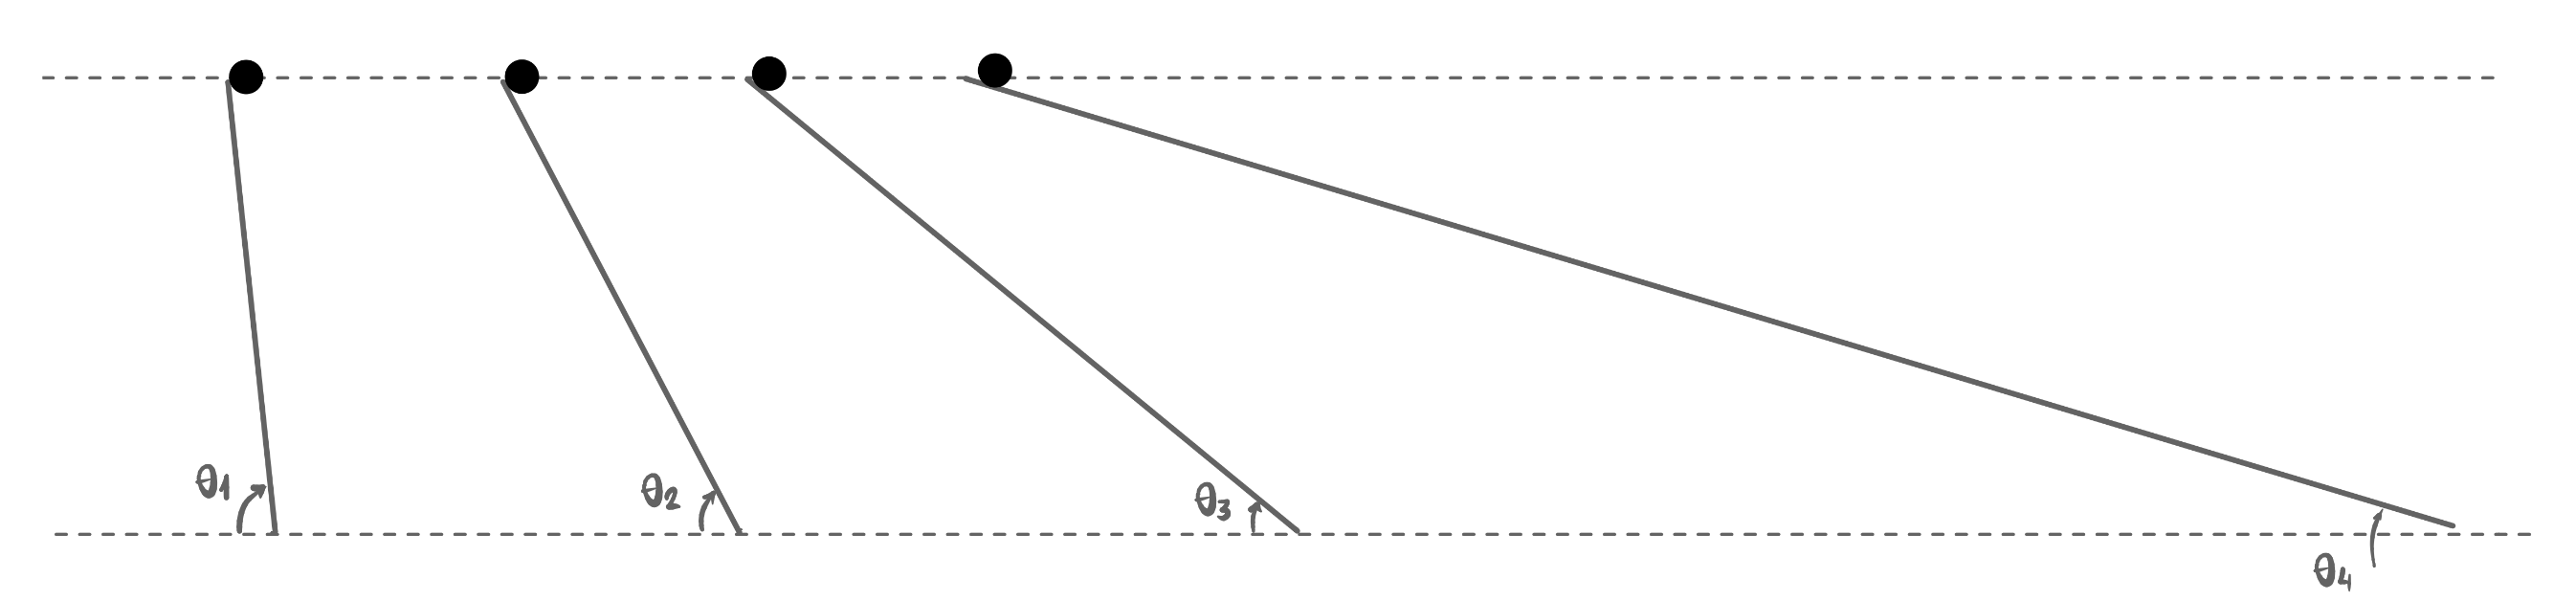
\includegraphics[width=1.0\linewidth]{imagensenergia/trabalhopesoconservativo4.png}
\captionof{figure}{Qual é a velocidade com que a bolinha chega ao final de cada rampa?}
\label{fig_energia_trabalhopesoconservativo4}
} 
\vspace{0.3cm}


Ora, façamos o cálculo para um caso específico, digamos, para o ângulo de inclinação $\theta_2.$ Até aqui, sabemos que o trabalho da força peso será responsável por variar a energia cinética da bolinha. Assim, para determinar sua velocidade final (que está associada à sua energia cinética final) basta descobrir, portanto, o trabalho da força peso ao longo de cada percurso. Ora, como já sabemos do estudo do plano inclinado, feito no desenvolvimento da Equação \eqref{eq_dinamicanewtoniana_gsintheta}, a componente da força responsável por acelerar a bolinha (e, portanto, por aumentar sua energia cinética) é a componente $P \sin \theta_2,$ como mostra a Figura \ref{fig_energia_trabalhopesoconservativo3}.

\vspace{0.3cm}
{
\centering
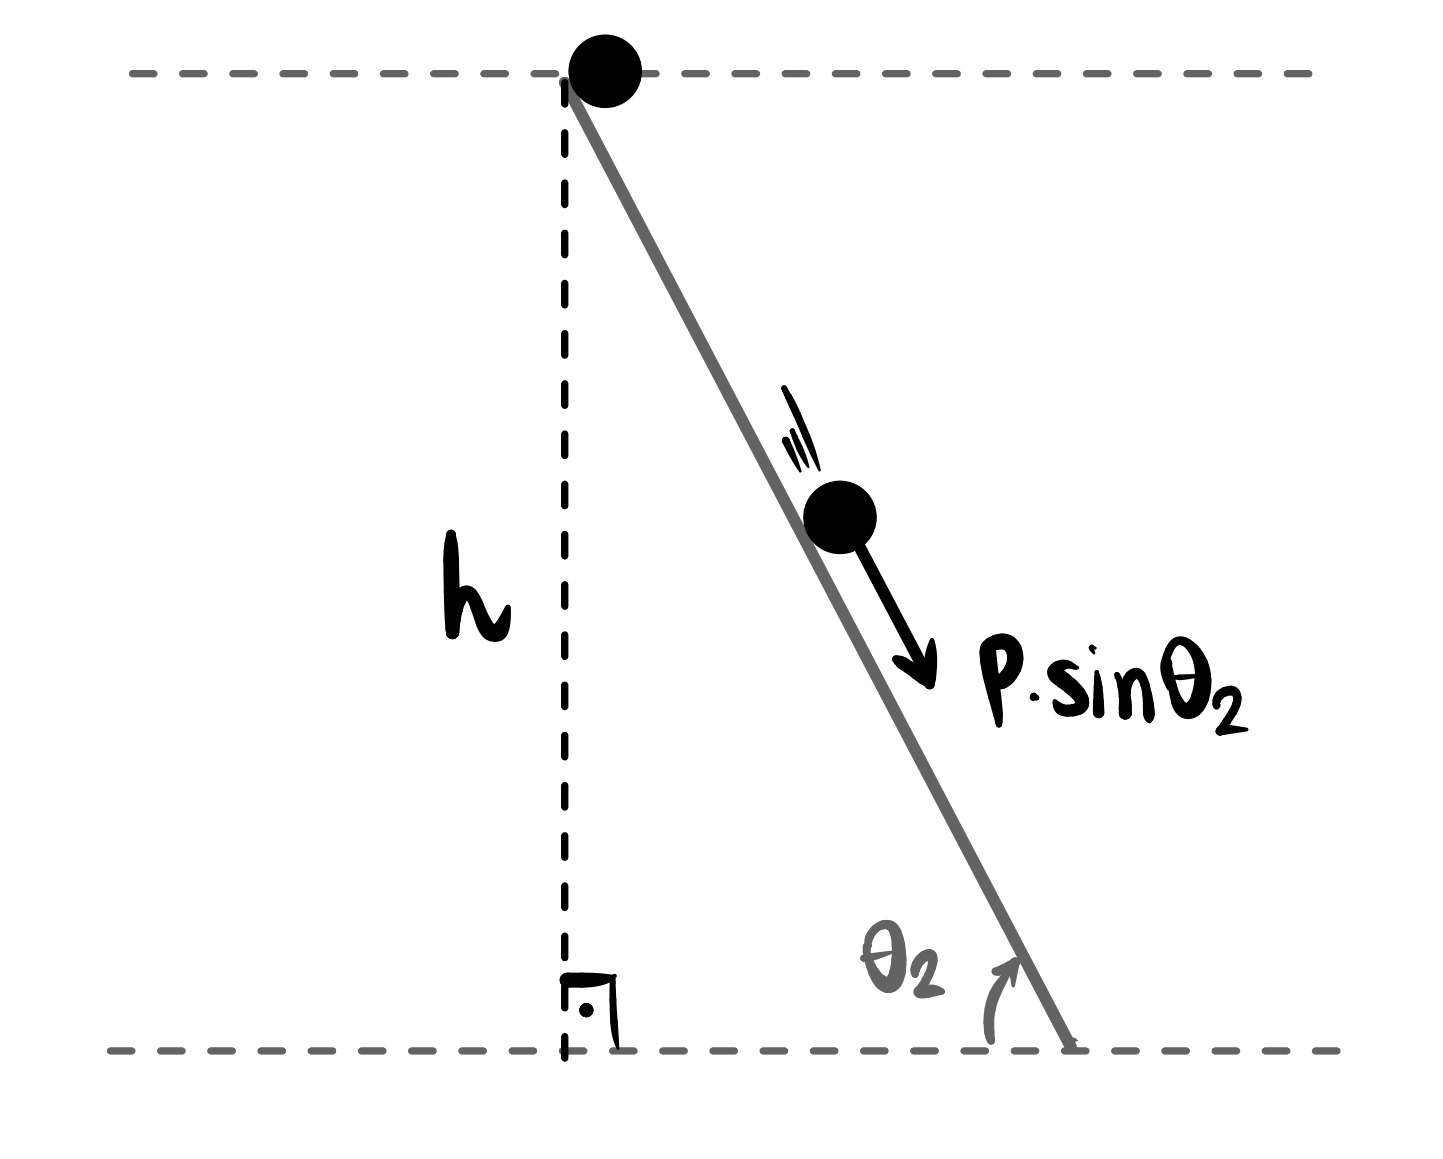
\includegraphics[width=0.3\linewidth]{imagensenergia/trabalhopesoconservativo3.png}
\captionof{figure}{Calculando o trabalho ao longo do deslocamento pela rampa 2.}
\label{fig_energia_trabalhopesoconservativo3}
} 
\vspace{0.3cm}

Assim, como a normal não realiza trabalho, o trabalho total será exclusivamente devido à força gravitacional (o peso), que é dado por:

$$ W_P = P_{//} \cdot d = P \sin \theta_2 \cdot d_2 = mg\sin \theta_2 \cdot d_2,$$

\noindent e, pela definição de seno no triângulo retângulo, tem-se $\sin \theta_2 = h/d_2$, de onde segue que

$$  W_P =  mg \cdot \dfrac{h}{\cancel {d_2}} \cdot \cancel {d_2} = mgh.$$

O que ocorreu acima é bem sutil, e vale ser destrinchado. Note que o trabalho acabou não dependendo do deslocamento $d$ que a bola sofre ao longo da rampa: ele cancelou. Assim, para qualquer ângulo $\theta_i$ das rampas da Figura \ref{fig_energia_trabalhopesoconservativo4} o trabalho será exatamente o mesmo: ele depende apenas de $m,$ $g$ e do desnível $h$ sofrido pela bolinha.

O que aconteceu, em mais detalhes, foi o seguinte: sendo o trabalho da força peso dado pelo produto $W_P = P_{//} \cdot d,$ à medida que a rampa fica menos inclinada o deslocamento $d$ ao longo da rampa que a bolinha precisa ter para cair o mesmo tanto $h$ aumenta substancialmente -- é o caso da rampa de inclinação $\theta_4.$ Contudo, a componente do peso que realiza trabalho, $P_{//} = P \sin \theta,$ diminui muito à medida que se diminui a inclinação da rampa, haja vista que o seno diminui quando o ângulo diminui. O que acontece é que esses dois efeitos ocorrem de forma exata a se compensarem: o deslocamento ao longo da rampa aumenta, dado por:\footnote{Como $\sin \theta$ é um número entre 0 e 1, dividir por tal fator faz o número aumentar.}

$$ \sin \theta = \dfrac{h}{d} \implies d = \dfrac{h}{\sin \theta},$$

\noindent ou seja, o fator de aumento do deslocamento $d$ é justamente o inverso do fator de diminuição da componente do peso que realiza trabalho: $\sin \theta.$ É por isso que, para qualquer rampa, o trabalho será sempre o mesmo: a inclinação $\theta$ da rampa desaparece no cálculo do trabalho:

$$ W_P = P_{//} \cdot d = \underbrace{(P \cdot \cancel{\sin \theta})}_{P_{//}} \cdot \underbrace{\left(\dfrac{h}{\cancel{\sin \theta}} \right)}_{d}  = P \cdot h = mgh.$$

Com isso, como $W_P=W$, isto é, o trabalho total é igual ao trabalho da força peso neste contexto, pelo teorema da energia cinética, teremos

$$ W = \Delta E_C = \dfrac{1}{2}mv^2 - \dfrac{1}{2}m0^2\implies mgh = \dfrac{1}{2}mv^2 \implies \boxed{v=\sqrt{2gh},}$$

\noindent e a bola, nos quatro casos da Figura \ref{fig_energia_trabalhopesoconservativo4}, chega ao fim de cada rampa com a mesma velocidade.

O resultado que construímos parece interessante demais para pararmos por aqui. O que vimos foi que o trabalho da força peso \emph{independe do caminho tomado} (pelo menos para rampas retilíneas): ele depende apenas do desnível $h$ entre os dois pontos em questão, não importando se os dois pontos são conectados por uma rampa de maior ou de menor inclinação. Será que isso valeria para qualquer outro tipo de rampa?

Considere, por exemplo, a rampa da Figura \ref{fig_energia_trabalhopesoconservativo2}, formada por uma curva de formato qualquer. Ora, podemos compor tal curva exatamente pelos mesmos planos inclinados de inclinações $\theta_1, \theta_2, \theta_3, \text{ e } \theta_4$ da Figura \ref{fig_energia_trabalhopesoconservativo4}. A segunda imagem da Figura \ref{fig_energia_trabalhopesoconservativo2} mostra essa situação. 


\vspace{0.3cm}
{
\centering
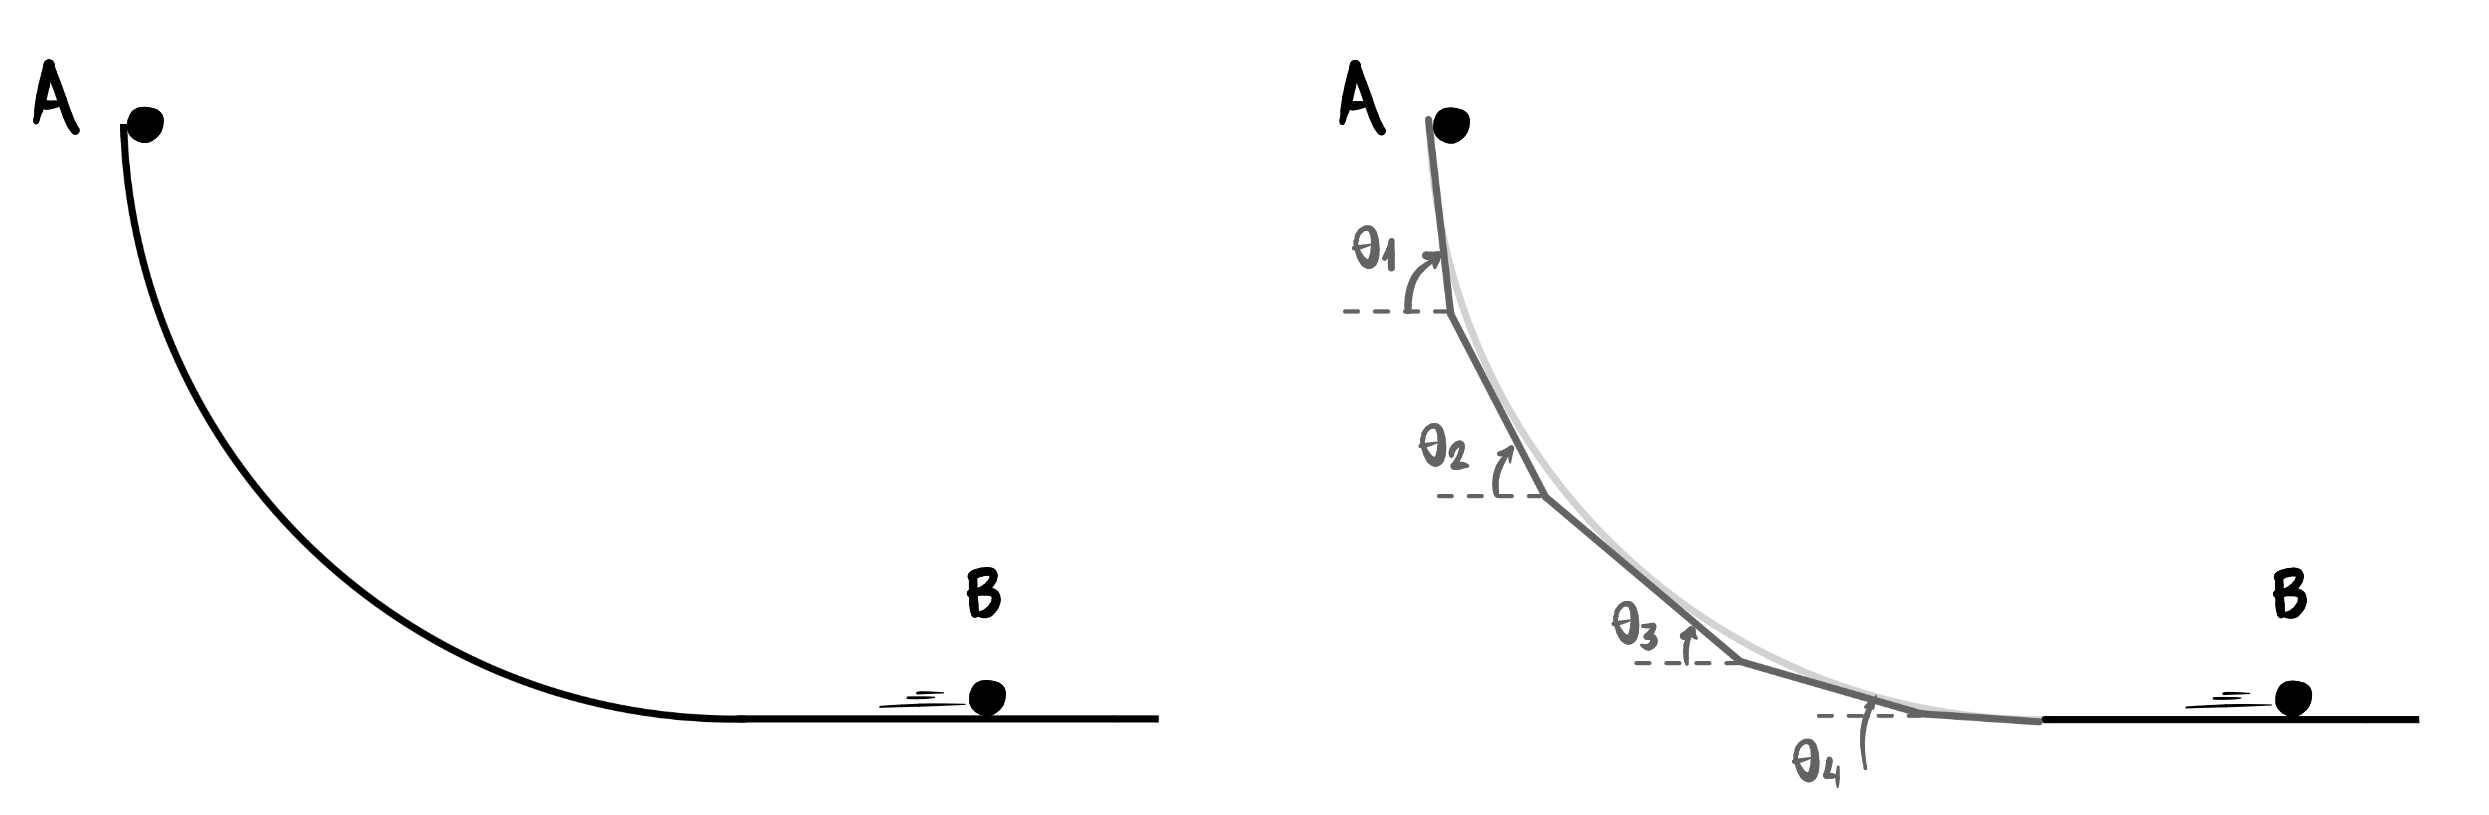
\includegraphics[width=0.9\linewidth]{imagensenergia/trabalhopesoconservativo2.png}
\captionof{figure}{Trabalho do peso ao longo de uma rampa qualquer.}
\label{fig_energia_trabalhopesoconservativo2}
} 
\vspace{0.3cm}


Sendo assim, já sabemos que o trabalho do peso em cada \emph{pedaço da rampa} (que está sendo interpretada como formada por vários planos inclinados) é dado por $W_i=mgh_i,$ em que $h_i$ é o desnível vertical sofrido pela bolinha ao escorregar o plano inclinado. 

\vspace{0.3cm}
{
\centering
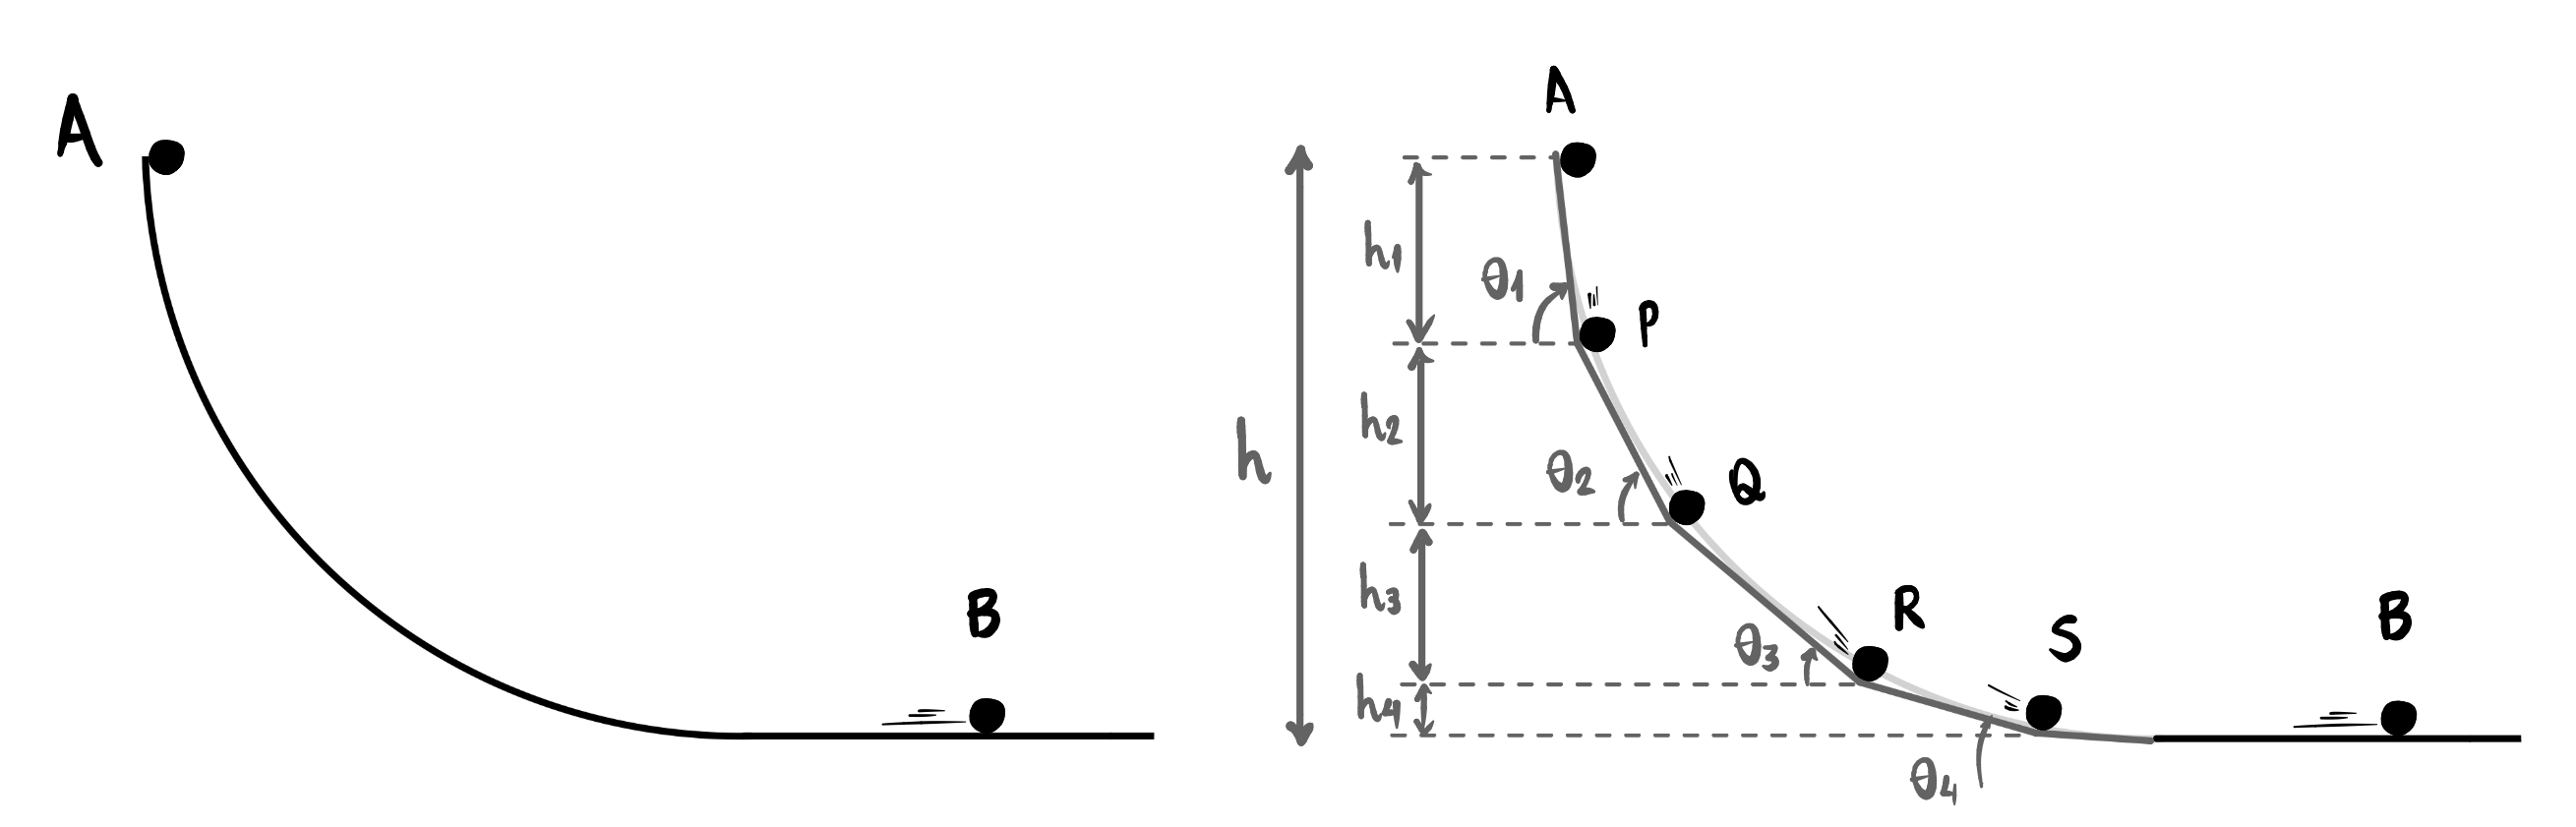
\includegraphics[width=0.9\linewidth]{imagensenergia/trabalhopesoconservativo6.png}
\captionof{figure}{Um rampa de formato qualquer pode ser interpretada como composta por uma sucessão de planos inclinados cujas inclinações variam ponto a ponto.}
\label{fig_energia_trabalhopesoconservativo6}
} 
\vspace{0.3cm}



Assim, os trabalhos da força peso em cada trecho seriam:

\begin{align}
    \text{A $\rightarrow$ P} &: W_1 = mgh_1 \nonumber \\
    \text{P $\rightarrow$ Q} &: W_2 = mgh_2 \nonumber \\
    \text{Q $\rightarrow$ R} &: W_3 = mgh_3 \nonumber \\
    \text{R $\rightarrow$ S} &: W_4 = mgh_4 \nonumber \\
     \text{S $\rightarrow$ B} &: W_5 = mgh_5 \nonumber,
\end{align}

\noindent em que, no último trecho S $\rightarrow$ B, o desnível $h_5$ é tão pequeno que sequer foi possível representá-lo na Figura \ref{fig_energia_trabalhopesoconservativo6}.

Ora, somando todas essas equações teremos o trabalho total realizado pela força peso no deslocamento da bolinha do ponto inicial $A$ até o ponto final $B:$

$$W_P = W_1 + W_2 + \dots +W_5 = mg(h_1+h_2 + \dots +h_5) = mgh,$$

\noindent uma vez que o desnível vertical total $h$ de $A$ até $B$ é igual à soma dos desníveis verticais em cada trecho: $h = h_1 + h_2 + \dots +h_5. $

Talvez o leitor pense que isso é só uma aproximação, haja vista que a curva não é exatamente composta pelas 5 rampas em questão. Contudo, podemos segmentar e dividir a curva em quantos trechos retilíneos quanto quisermos, como mostra a Figura \ref{fig_energia_trabalhopesoconservativo1}, para 10 planos inclinados diferentes sendo usados para compor a curva. 



\vspace{0.3cm}
{
\centering
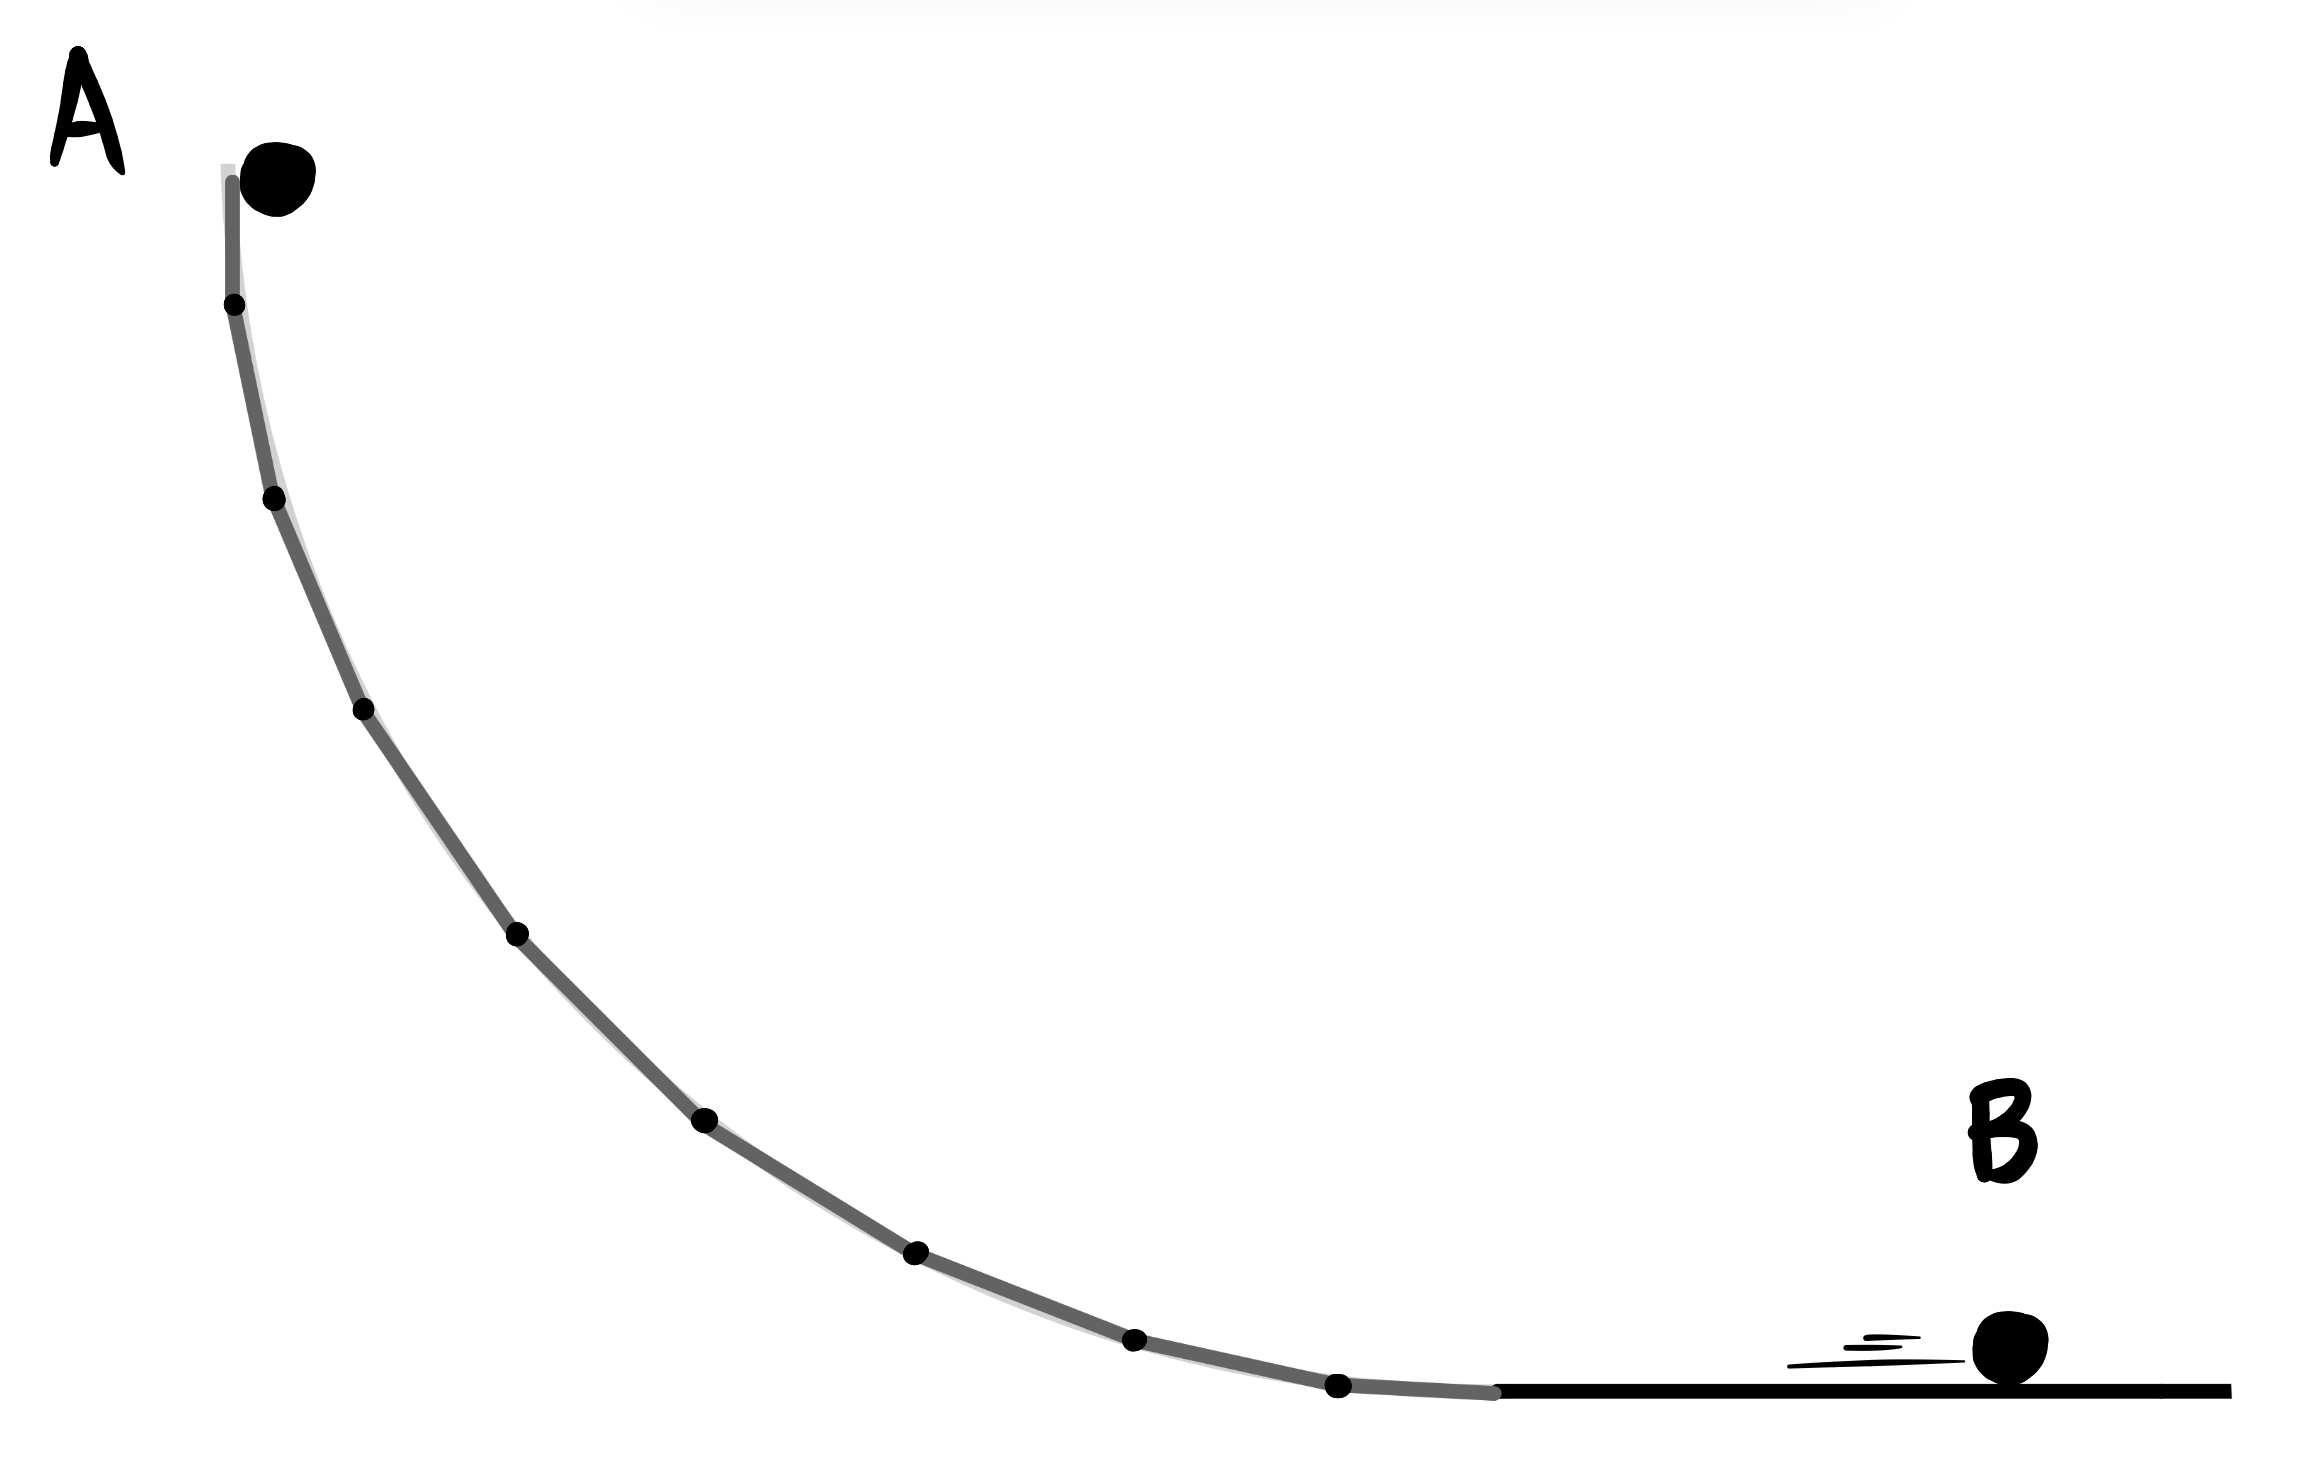
\includegraphics[width=0.6\linewidth]{imagensenergia/trabalhopesoconservativo1.png}
\captionof{figure}{Uma rampa de formato qualquer pode ser interpretada como formada por uma composição de vários planos inclinados.}
\label{fig_energia_trabalhopesoconservativo1}
} 
\vspace{0.3cm}




O leitor há de se convencer, observando essa figura, do segundo tópico abaixo, que concluirá a nossa argumentação:

\begin{enumerate}
    \item [(i)] O trabalho da força peso ao longo de um deslocamento quando um corpo desce por uma rampa retilínea qualquer é sempre o mesmo, dado por $W_P=mgh,$ dependendo apenas do desnível vertical $h$ dos pontos inicial e final do movimento, e não da inclinação $\theta$ da rampa. Isso já foi provado por nós.

    \item [(ii)] Uma curva de um formato qualquer pode ser interpretada como composta por pequenas rampas retilíneas (pequenos planos inclinados), de onde concluí-se que o trabalho da força peso ao longo do deslocamento por uma curva qualquer depende, como no caso dos planos inclinados, apenas do desnível vertical $h$ entre os pontos inicial e final do movimento, sendo dado, portanto, por $W_P = mgh.$
\end{enumerate}




\emph{Eureka}! A conclusão que chegamos aqui é digna de se sair correndo pelado nas ruas, gritando Eureka, como a história conta ter sido feito por Arquimedes ao descobrir, durante um banho em sua banheira, a lei do empuxo.\footnote{O leitor verá essa história no desenvolvimento da Equação \eqref{eq_fluidos_empuxo}. Até lá, recomenda-se seguir os estudos vestido.}
O que acabamos de descobrir é que \textit{o trabalho da força peso independe do caminho tomado: essa força, sendo vertical, depende apenas do desnível vertical $h$ dos pontos extremos do deslocamento da partícula.} Isso é um feito tão raro que merece um nome específico: forças que satisfazem essa condição são chamadas de \emph{forças conservativas.}\footnote{O atrito cinético, por outro lado, é o exemplo de força
não-conservativa --- também chamada dissipativa. O
trabalho do atrito depende sim do caminho: um percurso mais longo
implica mais atrito, mais trabalho dissipado. Num percurso fechado, o
trabalho do atrito não é zero --- ele é negativo, e seu módulo cresce
com o comprimento do trajeto. É precisamente por isso que o atrito
``destrói'' energia cinética ao convertê-la em calor.} Como mostra a Figura \ref{fig_energia_forcaconservatica}, o trabalho de uma força conservativa (como o peso) quando uma partícula se desloca entre os pontos $A$ e $B$ é sempre o mesmo: ele independe do caminho, dependendo apenas dos pontos inicial e final. 

\vspace{0.3cm}
{
\centering
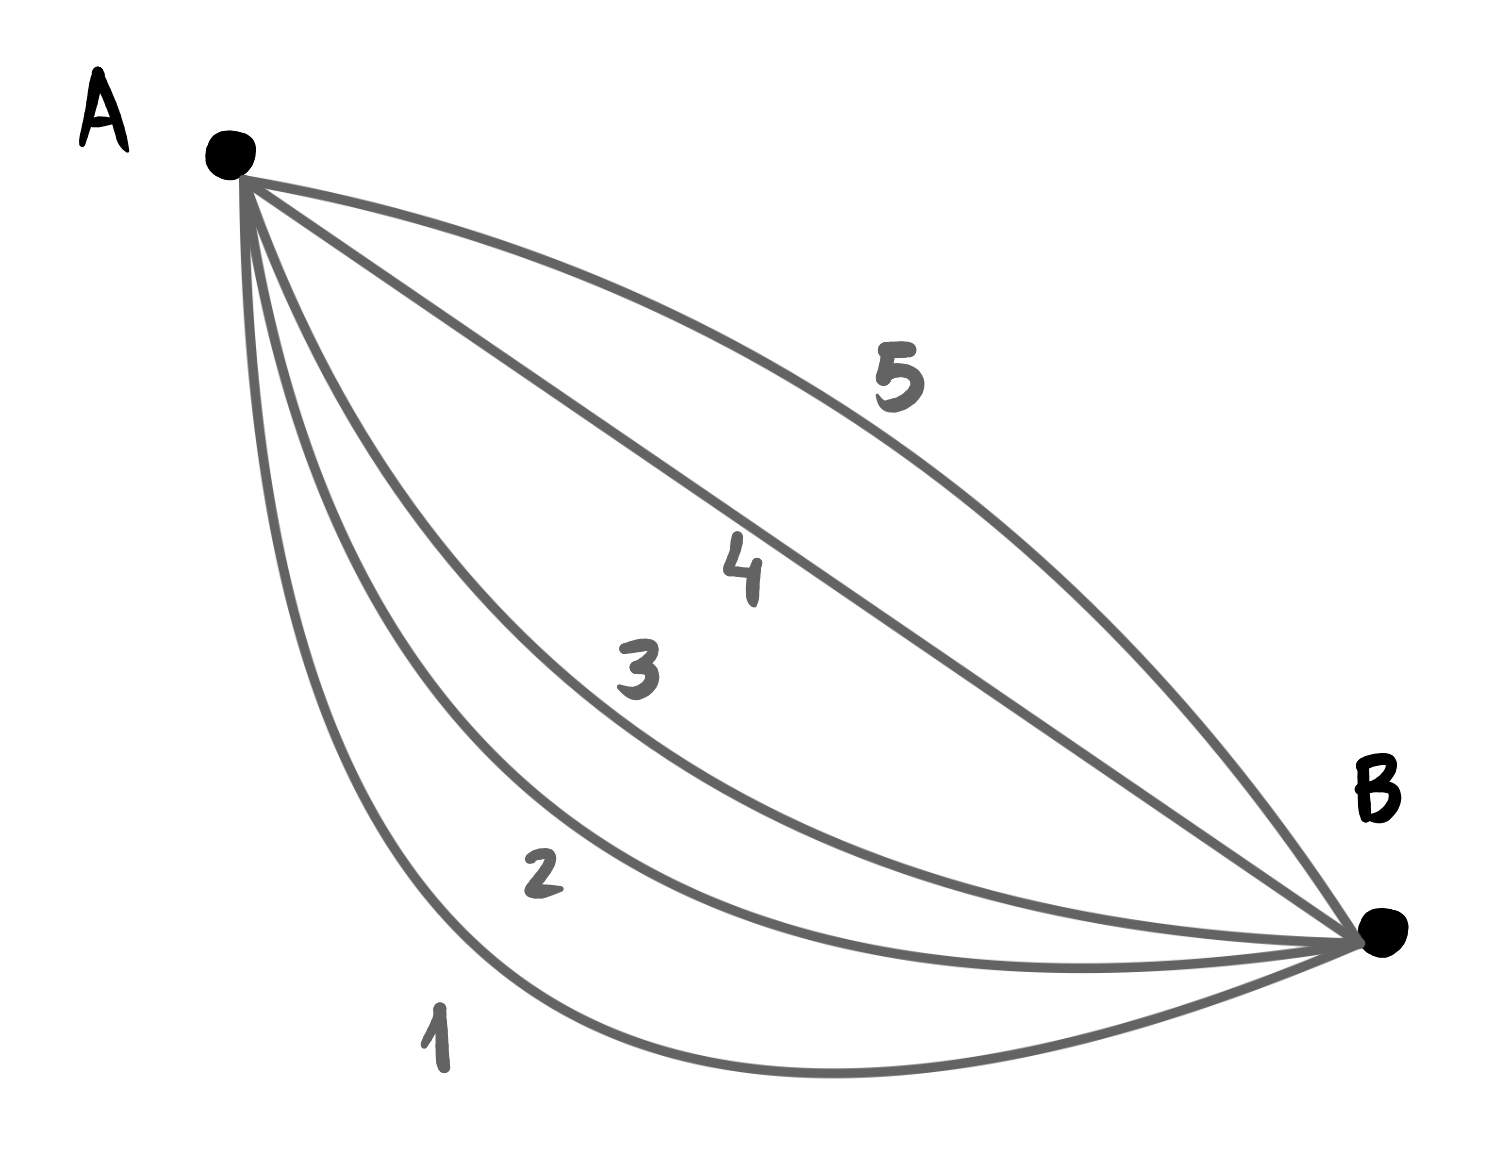
\includegraphics[width=0.4\linewidth]{imagensenergia/forcaconservatica.png}
\captionof{figure}{O trabalho de uma força conservativa depende apenas dos pontos inicial e final, $A$ e $B,$ e não do caminho.}
\label{fig_energia_forcaconservatica}
} 
\vspace{0.3cm}

No caso do peso, especificamente, o trabalho depende do desnível vertical $h$ entre os pontos finais $A$ e $B:$ $h=h_A-h_B.$ Para o caso da Figura \ref{fig_energia_forcaconservatica}, o trabalho do peso é o mesmo quer a bolinha escorregue por qualquer uma das cinco rampas.


Dessa forma, para computar o trabalho de uma força que satisfaz tal condição, há um caminho mais fácil do que aplicar diretamente o cálculo da definição de trabalho, dada pela Equação \eqref{eq_energia_trabalho}. Como nós vimos, para uma força conservativa, basta computar o trabalho para um caminho qualquer entre $A$ e $B$, e o trabalho da força em qualquer outro caminho que conecta esses dois pontos é sempre o mesmo. 

Note que, para os diferentes caminhos da Figura \ref{fig_energia_forcaconservatica}, o tempo que a bolinha levará para escorregar de $A$ até $B$ será diferente em cada caminho; a distância percorrida também é específica de cada caminho; as forças, acelerações e velocidades em cada ponto serão também únicas para cada caminho. Assim, o fato de existir uma grandeza -- o trabalho da força peso -- que é exatamente o mesmo independente da trajetória é algo bem peculiar que merece destaque. Este será o ponto principal que permitirá uma formulação alternativa da dinâmica que seja mais simples. 

Assim, para a força peso, podemos definir uma função chamada de \emph{energia potencial gravitacional}, dada por $E_P=mgh$, em que $h$ é o nível em que a massa $m$ se encontra em relação a alguma referência. Esse nível de referência é arbitrário, mas normalmente escolhemos como sendo o solo -- o nível mais baixo no contexto do problema. 



\vspace{0.3cm}
{
\centering
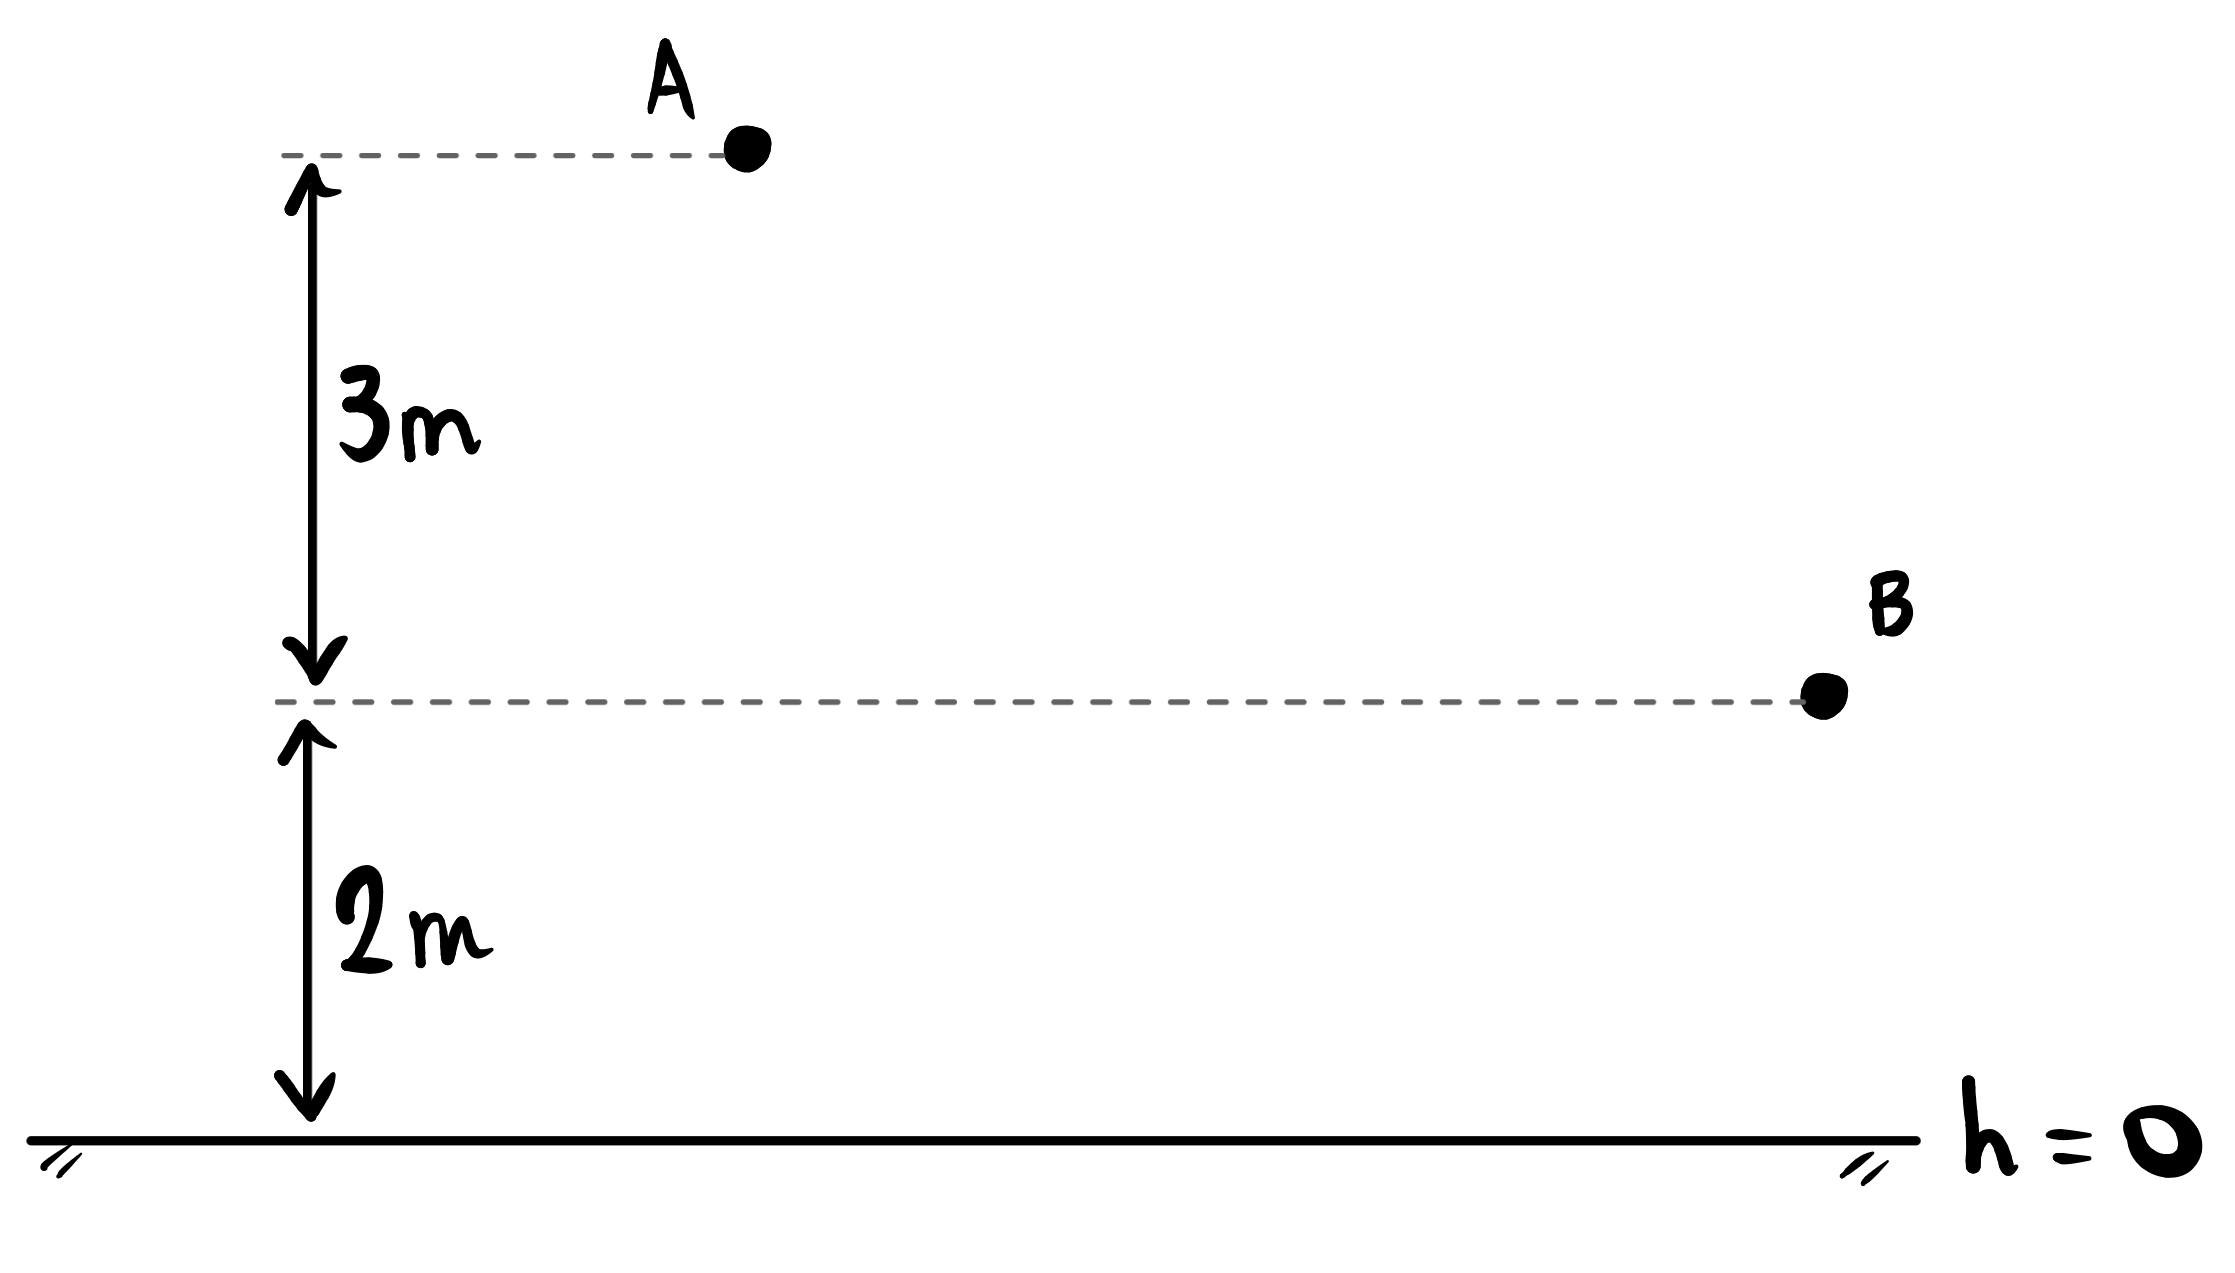
\includegraphics[width=0.4\linewidth]{imagensenergia/definicaoepot1.png}
\captionof{figure}{Cálculo da energia potencial de uma partícula nos pontos $A$ e $B$.}
\label{fig_energia_definicaoepot1}
} 
\vspace{0.3cm}

No caso da Figura \ref{fig_energia_definicaoepot1}, para uma massa $m = 1$kg, teríamos:

\begin{align}
    E_{\text{P}_A} &= mgh_A = 1 \cdot 10 \cdot 5 = 50 \text{J} \nonumber \\
    E_{\text{P}_B} &= mgh_B = 1 \cdot 10 \cdot 2 = 20 \text{J}, \nonumber 
\end{align}

\noindent e, como sabemos, o trabalho da força peso quando a bolinha se desloca de $A$ até $B$ depende do desnível $\Delta h$ entre esses dois pontos, sendo dado por:

$$ W_P = mg \Delta h = mg (h_A - h_B) =  mgh_A -  mgh_B = E_{\text{P}_A} - E_{\text{P}_B} = -(E_{\text{P}_B} - E_{\text{P}_A}) = -\Delta E_P.$$

Ou seja, o trabalho é calculado através da \emph{variação da energia potencial}. No exemplo da Figura \ref{fig_energia_definicaoepot1}, teríamos

$$W_P = -\Delta E_P = -(20-50) = -(-30) = 30 \text{ J.}  $$

Essa relação é tão importante que merece um destaque a parte:


\begin{equation}
    \boxed{ W = -\Delta E_\text{P}}
    \label{eq_energia_trabalhoevariacaoenergiapotencial}
\end{equation}

A Equação \eqref{eq_energia_trabalhoevariacaoenergiapotencial} vale para qualquer força conservativa. Cada força conservativa possui uma energia potencial associada a ela, e o trabalho que essa força conservativa realiza quando uma partícula se desloca de um ponto inicial $i$ até um ponto final $f$ não depende do caminho entre esses pontos, mas apenas dos pontos inicial e final, de modo que o trabalho pode ser computado apenas sabendo o valor da energia potencial nesses extremos: $W = -\Delta E_P = -(E_{\text{P}_f} - E_{\text{P}_i}).$

Talvez o sinal negativo na Equação \eqref{eq_energia_trabalhoevariacaoenergiapotencial} possa incomodar o leitor em um primeiro momento. Por ora, retifico-o de que é isso mesmo: não há nenhum tipo de erro. A energia potencial é \emph{definida} de modo a satisfazer tal equação. O leitor entenderá as profundas consequências desse sinal negativo no estudo da Equação \eqref{eq_energia_conservacaodaenergiamecanica}.

Continuando na situação da Figura \ref{fig_energia_definicaoepot1}, ao conectar os pontos $A$ e $B$ por uma rampa qualquer, o trabalho da força peso será sempre de $30$ joules quando a partícula vai de $A$ até $B$.


\vspace{0.3cm}
{
\centering
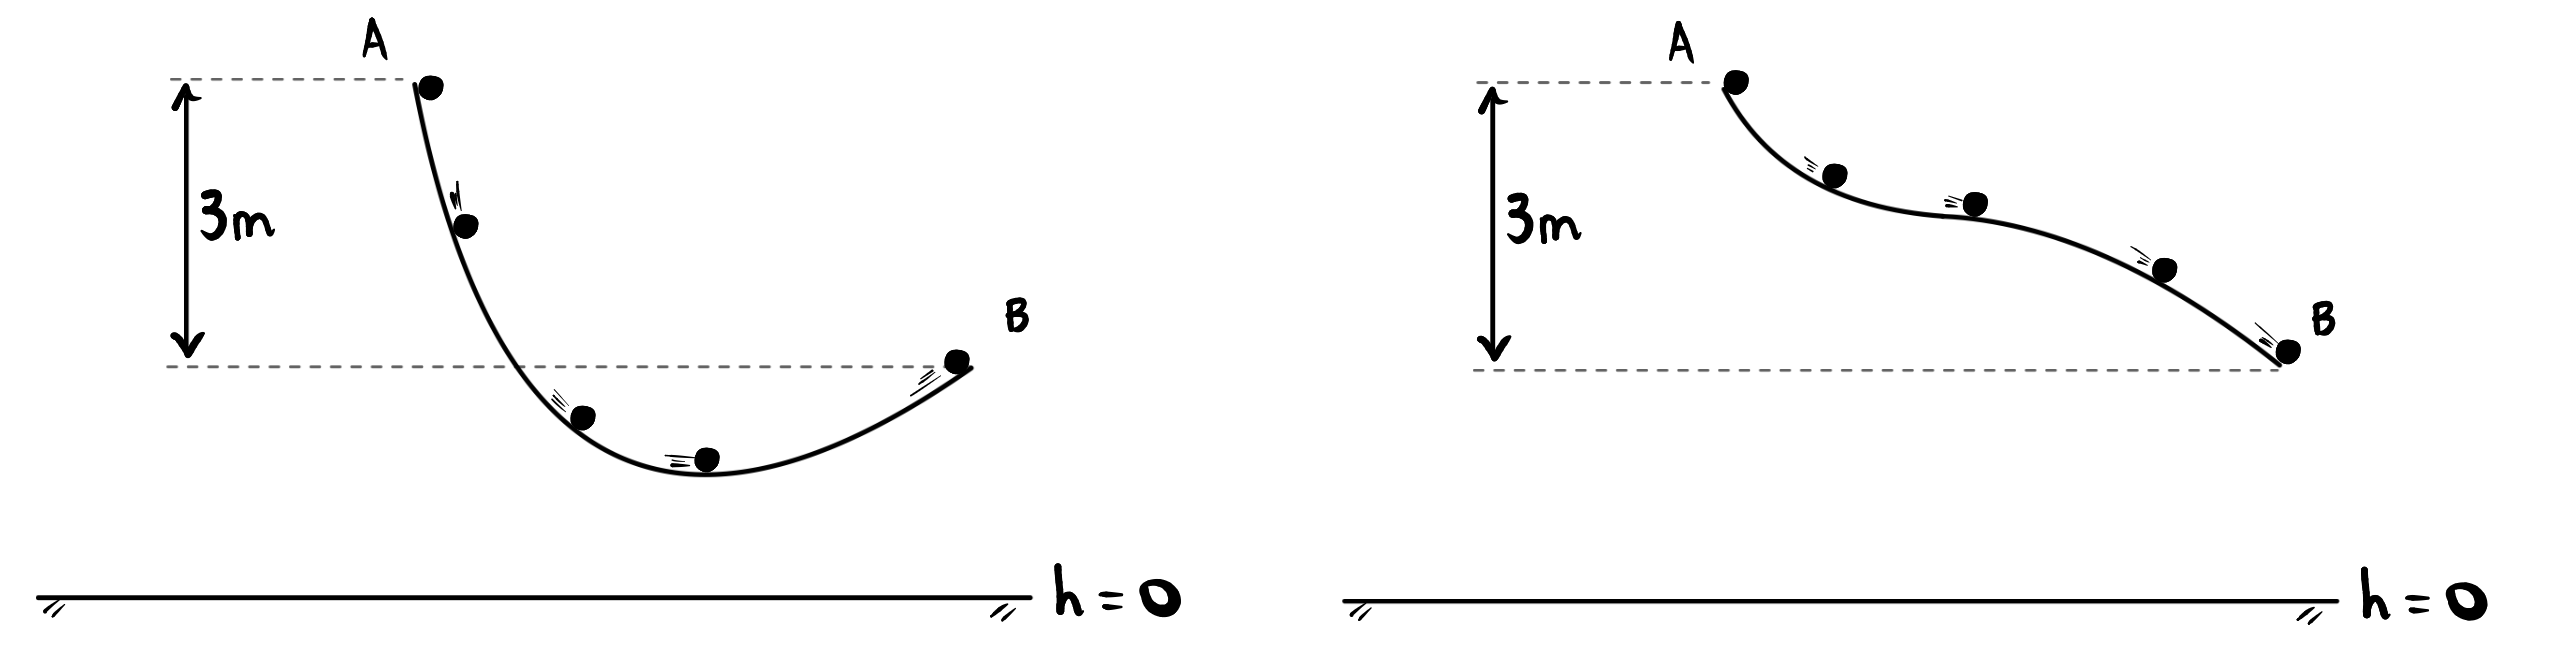
\includegraphics[width=0.9\linewidth]{imagensenergia/definicaoepot2.png}
\captionof{figure}{A velocidade final da partícula em $B$, sob ação de uma força conservativa, independe do caminho tomado.}
\label{fig_energia_definicaoepot2}
} 
\vspace{0.3cm}

Assim, pelo Teorema da Energia Cinética, como $W= \Delta E_C,$ teríamos que, saindo do repouso, a velocidade final em $B$ das bolinhas que percorrem os dois trechos da Figura \ref{fig_energia_definicaoepot2} seriam exatamente as mesmas, sendo dadas por:

$$ W = 30 = \Delta E_C \implies 30 = \dfrac{1}{2}mv_B^2 - \dfrac{1}{2}m \cancelto{0}{v_A^2} \implies 30 = \dfrac{1}{2} \cdot 1 \cdot v_B^2,$$

\noindent de onde segue que $v_B = \sqrt{60} \approx 7.74$ m/s.

Note que, até pouco tempo atrás, seria impossível que o leitor resolvesse este problema. Com as leis de Newton precisaríamos conhecer o formato específico das rampas da Figura \ref{fig_energia_definicaoepot2}, avaliar e decompor as forças em cada ponto para encontrar as acelerações e, com isso, compreender como a velocidade muda. A grande riqueza do conceito de força conservativa é justamente \emph{ignorar por completo o meio do caminho.} Como o trabalho de tal força depende apenas do ponto inicial e final, o formato específico da rampa é irrelevante, e toda a física do meio do caminho pode ser ignorada -- desde que apenas forças conservativas atuem  na partícula.

Essa foi uma seção um pouco maior do que o habitual, uma vez que estávamos definindo o conceito de força conservativa e de energia potencial, sendo a força peso (e a energia potencial gravitacional, associada a ela) o primeiro exemplo com o qual esbarramos. Tal conceito, portanto, é extremamente rico e nos possibilitará resolver vários problemas ignorando o meio do caminho e olhando apenas para os pontos inicial e final do movimento.


As demais forças conservativas com as quais o leitor terá contato a nível de Ensino Médio são a força gravitacional, a força elástica (que será estudada na próxima seção) e a força elétrica (que será estudada no Volume III dessa coleção).

Por fim, vale destacar a razão do nome de batismo dado a este conceito: \emph{energia potencial}. O nome não é arbitrário. A palavra \emph{potencial} vem do latim
\textit{potentia} --- capacidade, poder, aptidão para agir. Uma pedra
no alto de um morro não está em movimento, mas possui a \emph{capacidade}
de se mover: basta que seja liberada para que a gravidade se encarregue
de converter essa aptidão latente em velocidade real. A energia potencial
gravitacional mede exatamente isso --- não o que o corpo \emph{está
fazendo}, mas o que ele \emph{pode fazer} graças à sua posição no campo
gravitacional. É, portanto, uma energia de configuração: ela não reside
no movimento do objeto, mas na relação entre ele e a Terra. Quando o
objeto cai, essa capacidade se concretiza.

Assim, quando fazemos o cálculo da Figura \ref{fig_energia_definicaoepot1} e dizemos que a energia potencial da bolinha na posição $A$ (em relação ao solo) é de 50 joules, isso significa dizer que, naquela posição, a bolinha tem um \emph{potencial de adquirir 50 J de energia cinética}: caso abandonada, a bolinha aceleraria sob a ação da gravidade, realizando aquele seu potencial e adquirindo movimento, atingindo o solo com exatamente 50 joules de energia cinética.


\secgfe{Onde é usada}


A energia potencial gravitacional não é apenas uma ferramenta de
cálculo: ela é a linguagem com que a natureza contabiliza o trabalho
que a gravidade ainda está ``para fazer''. Suas aplicações permeiam
desde os problemas mais elementares do Ensino Médio até algumas das
maiores obras de engenharia já construídas pela humanidade.

O exemplo mais grandioso talvez seja o das usinas hidrelétricas. Uma
usina desse tipo é, em sua essência, uma máquina de converter energia
potencial gravitacional em energia elétrica. A água represada a uma
altura $h$ acima das turbinas possui energia potencial $E_p = mgh$;
ao ser liberada, ela desce, converte essa energia em cinética, e as
turbinas a transformam em eletricidade. A potência gerada depende
diretamente da vazão --- a massa de água que passa por segundo --- e
da chamada \emph{queda bruta}, que nada mais é do que a diferença de
altura entre o nível do reservatório e o das turbinas. Itaipu opera
com uma queda de aproximadamente \SI{120}{m}; Tucuruí, com cerca de
\SI{72}{m}. Essa diferença de altura mede, diretamente, a capacidade da usina produzir energia elétrica.

Uma extensão engenhosa do mesmo princípio é o chamado
\emph{bombeamento hidráulico reversível}, hoje uma das formas mais
eficientes de armazenar energia em larga escala. Quando há excesso
de eletricidade na rede --- durante a madrugada, por exemplo, quando
a demanda cai --- bombas elevam água de um reservatório inferior para
um superior, convertendo energia elétrica em potencial gravitacional.
Quando a demanda sobe, a água desce e o processo se inverte. O sistema
funciona como uma bateria gigantesca, e $E_p = mgh$ é exatamente a
fórmula que determina quanta energia pode ser armazenada em função da
massa d'água e da altura entre os dois reservatórios.

Descendo à escala humana, encontramos o pêndulo simples --- um dos
sistemas mais estudados na história da física e, durante séculos,
o coração dos relógios mecânicos. O pêndulo é um conversor cíclico
entre $E_p$ e $E_c$: no ponto mais alto de sua oscilação, toda a energia
é potencial; no ponto mais baixo, toda é cinética. Esse intercâmbio
periódico e regular foi reconhecido por Huygens em 1656 como um
mecanismo natural de medir o tempo, e os relógios de pêndulo que ele
inventou dominaram a relojoaria por mais de dois séculos. Toda a
análise quantitativa do pêndulo passa pela relação $E_p = mgh$, onde
$h$ é a altura do ponto de soltura em relação ao ponto mais baixo.

Na engenharia, a variação de energia potencial comparece sempre que
uma carga precisa ser elevada ou abaixada: guindastes, elevadores,
guinchos, planos inclinados de mineração. Quando um guincho eleva uma
carga de massa $m$ de uma altura $h_i$ até $h_f$, o trabalho mínimo
necessário é $\Delta E_p = mg(h_f - h_i)$, independentemente do
caminho percorrido --- consequência direta da propriedade conservativa
da força gravitacional que discutimos na seção anterior. Qualquer trabalho
adicional além desse mínimo é dissipado por atrito ou ineficiências
do mecanismo.

Dentro do próprio livro, $E_p$ reaparece como um dos dois pilares da
energia mecânica total, $E_m = E_c + E_p$, que estudaremos em uma seção
futura. Toda a análise de sistemas conservativos --- quedas livres,
montanhas-russas, projéteis, sistemas de polias --- depende desta
grandeza como parcela central da equação de conservação. 

% \medskip
% \noindent\textbf{Usinas hidrelétricas:} uma usina hidrelétrica é, em
% sua essência, uma máquina de converter energia potencial gravitacional
% em energia elétrica. A água represada a uma altura $h$ acima das
% turbinas possui energia potencial $E_p = mgh$; ao ser liberada, ela
% desce, converte essa energia em cinética, e as turbinas a convertem
% em energia elétrica. A potência gerada depende diretamente da vazão
% (massa de água por segundo) e da altura de queda --- chamada de
% \emph{queda bruta}. Itaipu, por exemplo, opera com uma queda de
% aproximadamente \SI{120}{m}; a usina de Tucuruí, com cerca de
% \SI{72}{m}. A diferença de altura não é um detalhe arquitetônico: ela
% é o reservatório de onde toda a energia elétrica gerada provém.

% \medskip
% \noindent\textbf{Armazenamento de energia por bombeamento:} uma das
% formas mais eficientes de armazenar energia em larga escala é o
% chamado \emph{bombeamento hidráulico reversível}: quando há excesso de
% energia elétrica na rede (por exemplo, durante a madrugada, quando a
% demanda é baixa), bombas elevam água de um reservatório inferior para
% um superior, convertendo energia elétrica em potencial gravitacional.
% Quando a demanda aumenta, a água desce e o ciclo se inverte. O
% sistema funciona como uma bateria gigantesca --- e $E_p = mgh$ é
% exatamente a fórmula que determina quanta energia pode ser armazenada.

% \medskip
% \noindent\textbf{Pêndulos e relógios mecânicos:} o pêndulo simples é
% um conversor cíclico entre $E_p$ e $E_c$: no ponto mais alto da
% oscilação, toda a energia é potencial; no ponto mais baixo, toda é
% cinética. Esse intercâmbio periódico é a base de funcionamento dos
% relógios de pêndulo, inventados por Huygens em 1656, que dominaram
% a medição do tempo por mais de dois séculos.

% \medskip
% \noindent\textbf{Planos inclinados e sistemas de polias:} toda a
% análise energética de rampas, elevadores, guinchos e sistemas de
% polias --- tão presentes em engenharia civil e mecânica --- passa
% pela variação de $E_p$. Quando um guincho eleva uma carga de massa
% $m$ de uma altura $h_i$ até $h_f$, o trabalho mínimo necessário é
% exatamente $\Delta E_p = mg(h_f - h_i)$, independentemente do caminho
% percorrido.

% \medskip
% \noindent\textbf{Conservação da energia mecânica:}
% $E_p$ é um dos dois termos que compõem a energia mecânica total,
% $E_m = E_c + E_p$. Toda a análise de sistemas conservativos ---
% quedas livres, montanhas-russas ideais, pêndulos, lançamentos
% oblíquos --- depende desta grandeza como parcela central da equação. Veremos isso em mais detalhes na Equação \eqref{eq_energia_conservacaodaenergiamecanica}.

% \medskip
% \noindent\textbf{Gravitação Universal}: para grandes
% alturas, onde $g$ não pode ser considerado constante, a expressão
% $mgh$ é substituída pela energia potencial gravitacional universal, dada pela Equação \eqref{eq_newton_energiapotencialgravitacional}. A fórmula simples é o caso-limite desta
% expressão para variações de altura próximas à superfície terrestre.
% O mesmo conceito --- energia armazenada na configuração do sistema
% gravitacional --- governa a física dos satélites, das órbitas
% planetárias e da velocidade de escape.





\secgfe{Erros comuns}


Considere a situação da Figura \ref{fig_energia_variacaoepot1}, em que uma bola de massa $m=5$kg é abandonada em um campo gravitacional uniforme $g$, percorrendo uma distância $\Delta h = 3$m. Considere o problema de se computar o trabalho da força peso ao longo deste deslocamento. 

Ora, o leitor simplesmente computa $W = -\Delta E_p = -mg \Delta h = -5 \cdot 10 \cdot (-3) = 150 $J, o que está perfeitamente correto.\footnote{Perceba que $\Delta h<0$ uma vez que a altura final é menor que a inicial. Assim, a rigor, teríamos $\Delta h = -3$m, o que ``\emph{corrige}'' (ou melhor, compensa) o sinal negativo que existe na definição da energia potencial, fazendo com que o resultado final seja positivo, como esperado.}

\vspace{0.3cm}
{
\centering
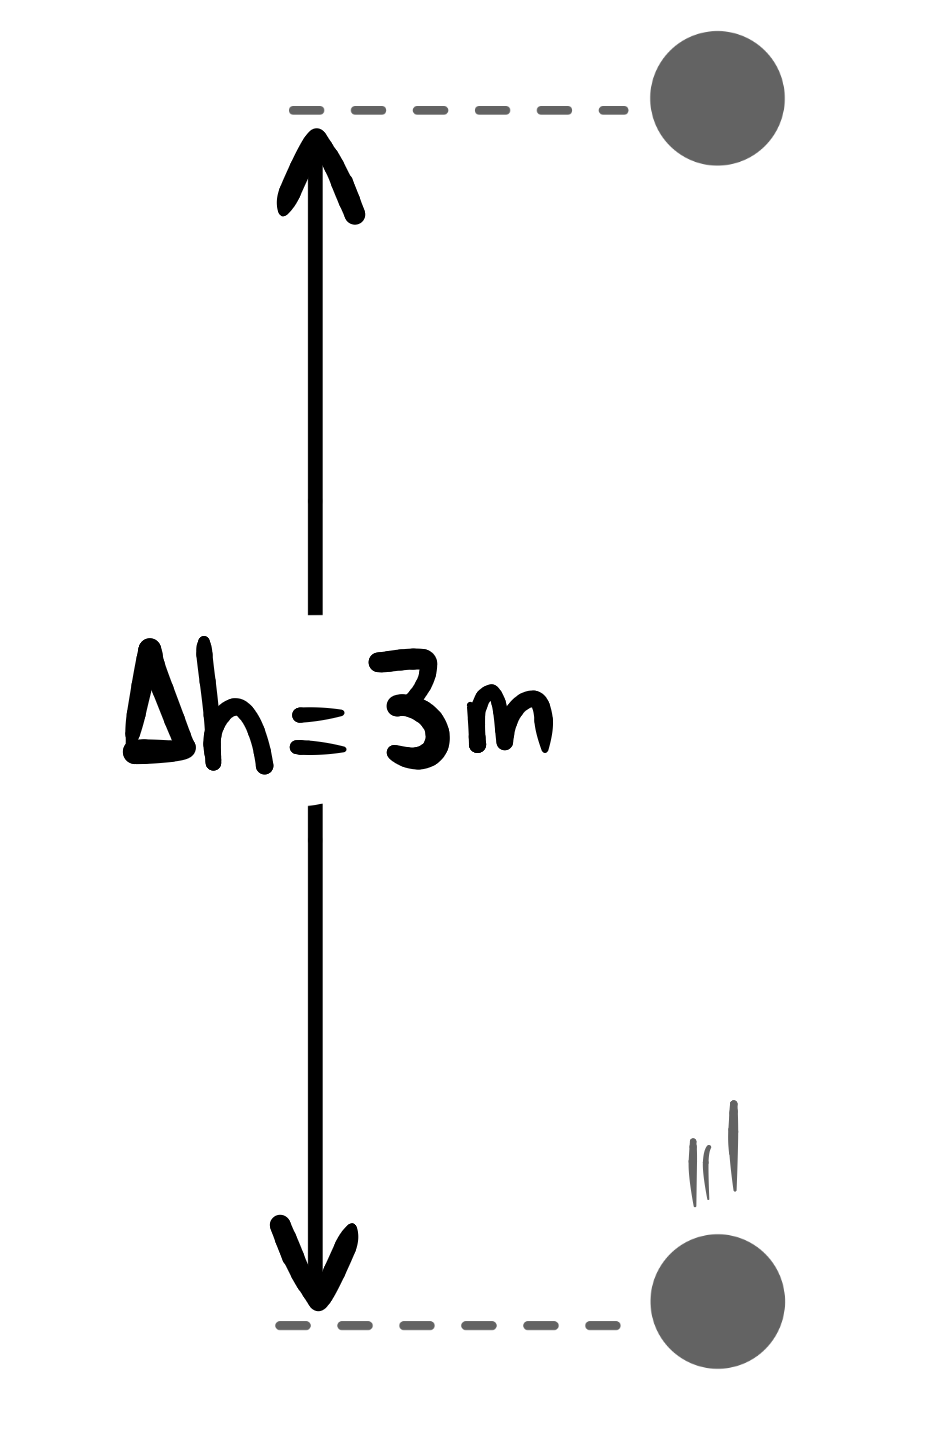
\includegraphics[width=0.2\linewidth]{imagensenergia/variacaoepot1.png}
\captionof{figure}{Bola abandonada em um campo gravitacional uniforme.}
\label{fig_energia_variacaoepot1}
} 
\vspace{0.3cm}

 A confusão começa a surgir na hora de se adotar o nível de referência. Para tanto, considere a Figura \ref{fig_energia_variacaoepot2}, que mostra exatamente a mesma situação da Figura \ref{fig_energia_variacaoepot1}, porém com diferentes níveis de referência para o cálculo da energia potencial gravitacional.



\vspace{0.3cm}
{
\centering
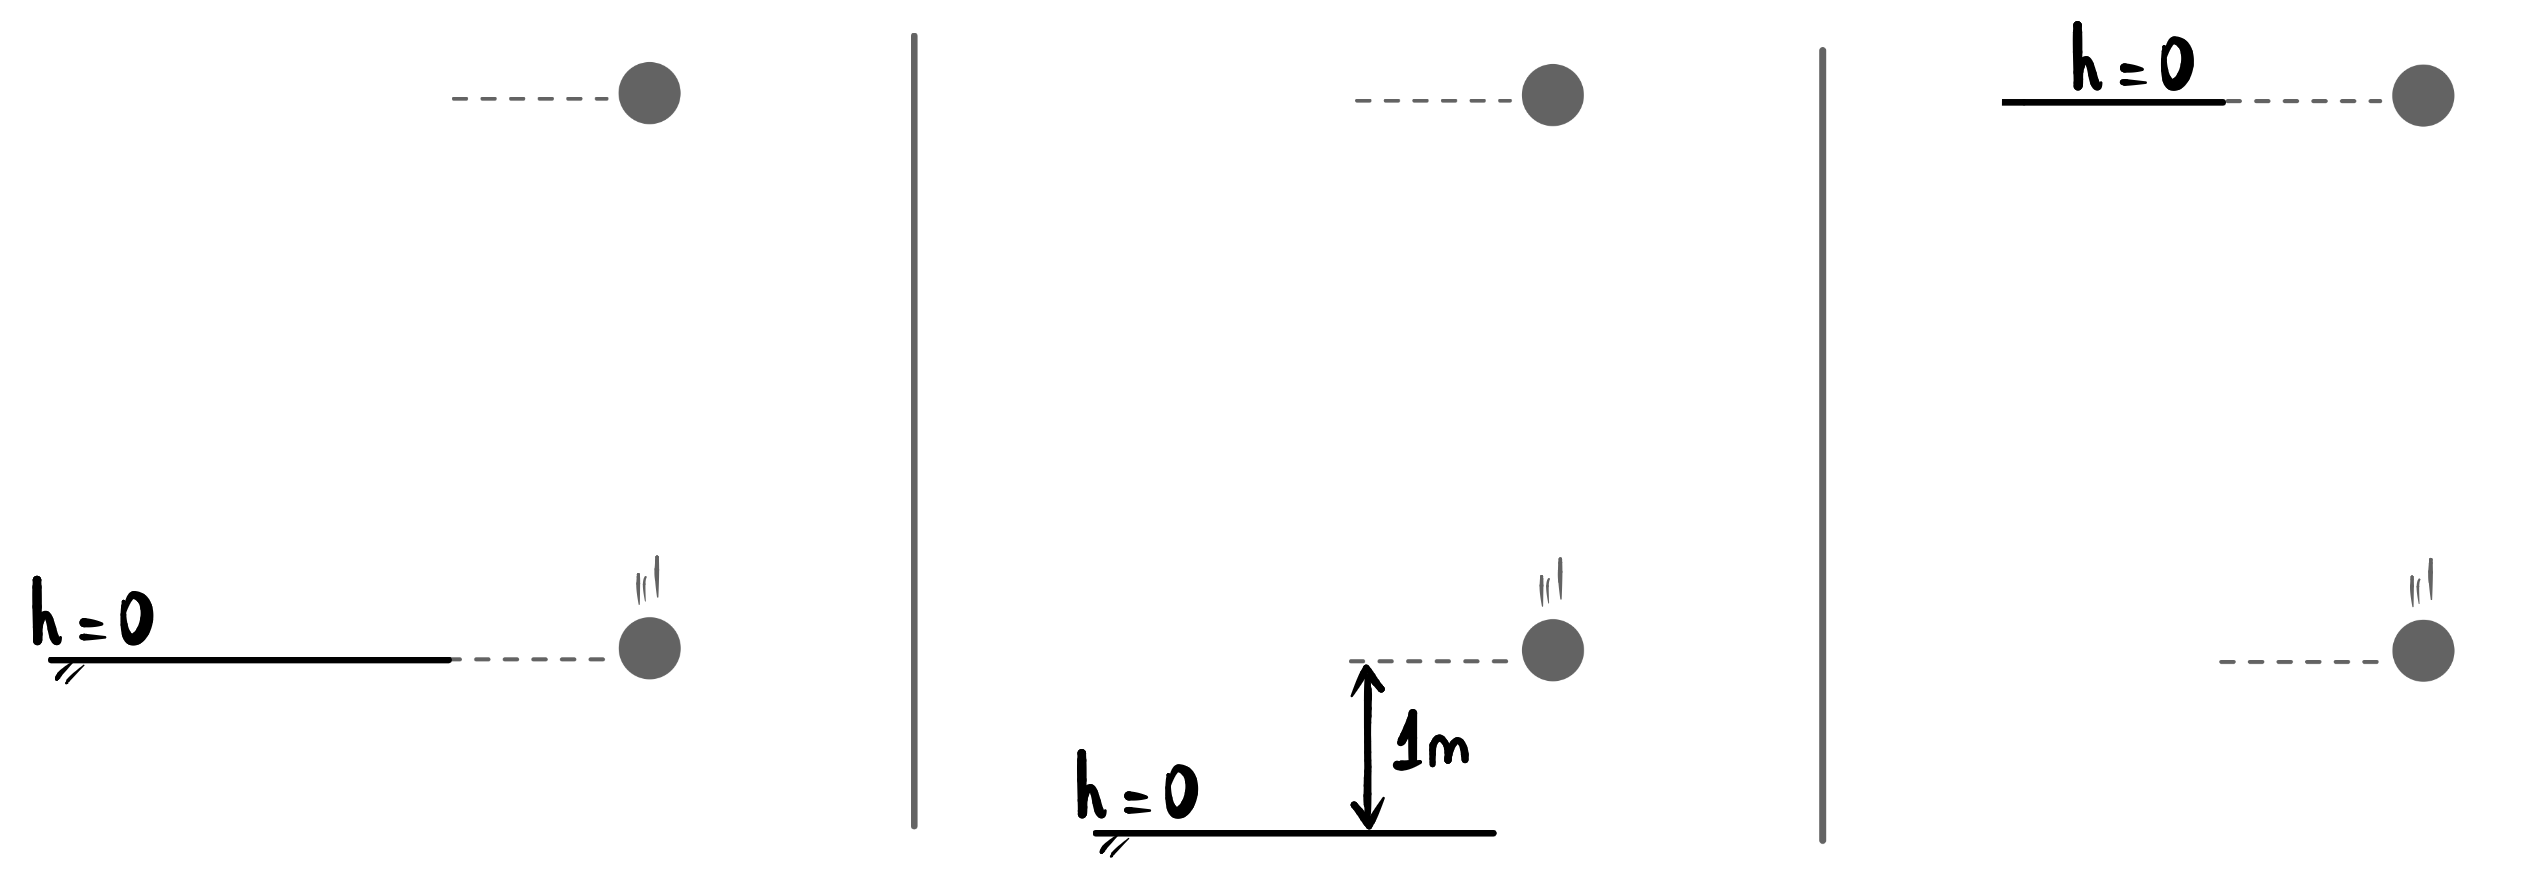
\includegraphics[width=0.9\linewidth]{imagensenergia/variacaoepot2.png}
\captionof{figure}{Adoção de diferentes níveis de referência para o cálculo da energia potencial gravitacional.}
\label{fig_energia_variacaoepot2}
} 
\vspace{0.3cm}

Seja $A$ a posição inicial do corpo e $B$ a sua posição após cair os três metros. Computemos a variação de energia potencial usando os diferentes níveis de referência da Figura \ref{fig_energia_variacaoepot2}:

\begin{enumerate}
    \item [(i)] Nível de referência ($h=0)$ na posição final da bolinha. Neste caso, as energias potenciais são:

    \begin{align}
        E_{\text{P}_A} &= mgh_A = 5 \cdot 10 \cdot 3 = 150 \text{J} \nonumber \\
          E_{\text{P}_B} &= mgh_B = 5 \cdot 10 \cdot 0 = 0 \text{J}, \nonumber 
    \end{align}

\noindent de modo que o trabalho da força peso ao longo desse deslocamento é:

$$ W = -\Delta E_P = -(0-150) = 150 \text{J,}$$

\noindent concordando com o valor esperado.
    

    \item [(ii)] Nível de referência ($h=0)$ no solo, que está 1 m abaixo da posição final da bolinha.  Neste caso, as energias potenciais são:

    \begin{align}
        E_{\text{P}_A} &= mgh_A = 5 \cdot 10 \cdot 4 = 200 \text{J} \nonumber \\
          E_{\text{P}_B} &= mgh_B = 5 \cdot 10 \cdot 1 = 50 \text{J}, \nonumber 
    \end{align}

\noindent de modo que o trabalho da força peso ao longo desse deslocamento é:

$$ W = -\Delta E_P = -(50-200) = -(-150) =150 \text{J,}$$

\noindent concordando com o valor esperado.

    \item [(iii)]   Nível de referência ($h=0)$ na posição inicial da bolinha. 

 Neste caso, as energias potenciais são:

    \begin{align}
        E_{\text{P}_A} &= mgh_A = 5 \cdot 10 \cdot 0 = 0 \text{J} \nonumber \\
          E_{\text{P}_B} &= mgh_B = 5 \cdot 10 \cdot (-3) = -150 \text{J}, \nonumber 
    \end{align}

\noindent de modo que o trabalho da força peso ao longo desse deslocamento é:

$$ W = -\Delta E_P = - (-150-0) = 150 \text{J,}$$

\noindent concordando com o valor esperado. Note, neste caso, que estando o ponto $B$ abaixo do ponto de referência em que $h=0$, sua altura é negativa (a altura $h$ cresce para cima e diminui para baixo, naturalmente).
    
\end{enumerate}

Nos três casos as energias potenciais nos pontos $A$ e $B$ tiveram valores distintos, contudo, a diferença entre elas -- que é a grandeza física relevante, que equivale ao trabalho do peso, pela Equação \eqref{eq_energia_trabalhoevariacaoenergiapotencial} -- deu sempre o mesmo valor. Assim, um erro comum é o leitor achar que o valor da energia potencial de um objeto em um ponto específico tem alguma importância. De fato, não tem. A energia potencial, por si só, não possui nenhum significado físico: é um valor arbitrário que depende de uma escolha arbitrária de referência, como ficou claro neste exemplo.\footnote{Inclusive, lanço um desafio ao leitor: medir a energia potencial de algum objeto em um ponto específico. Após pensar um pouco você verá que tal tarefa é impossível: é possível \emph{calcular} o valor da energia potencial de um objeto em um certo ponto, mas não é possível \emph{medir} a sua energia naquele ponto. Só é possível medir a \emph{diferença} de energia potencial, o que é feito, justamente, por meio da medida da velocidade do corpo, uma vez que a variação de energia potencial está associada ao trabalho do peso, que, por sua vez, está associado à variação de energia cinética do corpo. Isso mostra que o conceito de energia potencial é, em sua natureza, inerentemente abstrato. Somente a variação de energia potencial é concreta, pode ser medida e tem significado físico. Fica como reflexão para o leitor pensar sobre a diferença entre se \emph{calcular} uma grandeza e se \emph{medir} tal grandeza.}

Já a diferença de energia potencial será sempre a mesma, independente do sistema de referência adotado. Essa é a grandeza fisicamente relevante, e é por isso que o trabalho do peso está associado à \emph{variação da energia potencial}, e não à energia potencial em si. Assim, algum leitor poderia estranhar o fato de termos obtido energias potenciais negativas ou nulas em alguns casos acima. Contudo, lembre-se: a energia potencial de em ponto específico pode ter absolutamente qualquer valor (positivo, negativo ou zero) a depender do sistema de referência escolhido. O que tem importância, sempre, é a apenas a  \emph{variação da energia potencial}, e esta será sempre a mesma, para qualquer sistema de referência.



\secgfe{Observações}

Algumas observações merecem ser pontuadas a respeito da Equação \eqref{eq_energia_potencialgravitacional}:

\begin{enumerate}
    
    \item [(i)] Validade da expressão.

    Esta expressão é válida
  apenas quando $g$ pode ser considerado constante --- condição que se
  satisfaz para alturas muito menores que o raio da Terra
  ($R_T \approx \SI{6400}{km}$).
  
  O campo gravitacional $g$ varia com a distância ao centro da Terra, dado pela Equação \eqref{eq_newton_campogravitacional}. Assim, para satélites, foguetes, ou objetos
  em órbita, é necessário usar a expressão da gravitação universal para o cálculo da energia potencial gravitacional, dado pela Equação \eqref{eq_newton_energiapotencialgravitacional}. Durante o desenvolvimento dessa última equação, nós mostramos que, para $r$ próximo de $R_T$ com pequenas
  variações $\Delta r \ll R_T$, essa expressão se reduz a $mgh$ com o
  referencial na superfície.


    \item [(ii)] $E_p$ é uma propriedade do sistema que interage gravitacionalmente, não de um objeto isolado. Tecnicamente, a energia potencial gravitacional pertence ao sistema
  \emph{objeto + Terra}, não ao objeto isolado. É a interação entre os
  dois que armazena energia. Dados dois corpos massivos, ao abandoná-los, eles tendem a se aproximar um do outro, devido à interação gravitacional. Assim, ao começarem a se mover um em direção ao outro, eles ganham energia cinética, e isso só é possível porque havia energia potencial acumulada no sistema: uma energia com potencial de se converter em movimento.

No caso da Terra, como sua massa é muito maior do que a de qualquer corpo na sua superfície, ela praticamente não se move, de modo que podemos considerar que ela está parada e a energia potencial (e, portanto, a sua eventual conversão em energia cinética) é apenas do corpo em questão, e não do sistema corpo + Terra.
  
  



    \item [(iii)]  O termo ``energia potencial''
  foi introduzido pelo físico escocês William Rankine em 1853. Antes
  dele, Leibniz (no século XVII) já havia intuído a existência de uma
  forma de energia associada à posição, que ele chamava de
  \textit{vis mortua} (``força morta''), em oposição à \textit{vis
  viva} (``força viva'', proporcional a $mv^2$), precursora da energia
  cinética. Havia, portanto, uma intuição correta de que existiam duas
  ``moedas'' distintas com as quais a natureza realizava seus
  intercâmbios --- mas foi necessário mais de um século para que a
  linguagem matemática precisasse essa intuição.\footnote{O leitor
  curioso encontrará uma narrativa envolvente dessa história em
  \textit{The Mechanical Universe}, de Steven Frautschi et al., e
  em \textit{A História da Física}, de Isaac Asimov.}
    
\end{enumerate}




\vspace{0.3cm}

\begin{exemplo}[Nível I]\label{exemplo_energia_potencialgravitacionalex01}

Um livro de \SI{0{,}5}{kg} repousa sobre uma prateleira localizada a
\SI{1{,}2}{m} acima do chão. Adote $g = \SI{10}{m/s^2}$ e o chão como
referencial ($h = 0$). Calcule a energia potencial
gravitacional do livro.


\resolucao

A aplicação é direta: o livro está a uma altura
$h = \SI{1{,}2}{m}$ do referencial escolhido. Portanto:

\[
  E_p = mgh = 0.5 \cdot 10 \cdot 1.2 = \SI{6.0}{J}.
\]

Isso quer dizer que você gastaria exatamente $\SI{6{,}0}{J}$ de energia para erguer o livro do chão e colocá-lo sobre a prateleira. Quer dizer também que, se o livro cair, ele colide com o chão com uma energia total de $\SI{6{,}0}{J}$, que é o que irá ditar o impacto sofrido pelo chão por tal colisão.

\end{exemplo}

\vspace{0.3cm}





\begin{exemplo}[Nível II]\label{exemplo_energia_potencialgravitacionalex02}

Dois blocos idênticos, cada um de massa $m = \SI{2{,}0}{kg}$, são
soltos do repouso no topo de dois planos inclinados sem atrito de
mesma altura $h = \SI{5{,}0}{m}$, porém com ângulos diferentes:
$\theta_A = 30^\circ$ e $\theta_B = 60^\circ$. Adote $g = \SI{10}{m/s^2}$.

\begin{enumerate}
  \item  [a)]Qual é a velocidade de cada bloco ao chegar à base do
  respectivo plano?
  \item  [b)] O que o resultado nos diz sobre o papel do ângulo de
  inclinação num sistema sem atrito?
\end{enumerate}

\resolucao

\textit{a)} A única força que realiza trabalho sobre cada bloco é o peso (a normal
é perpendicular ao deslocamento e, portanto, não contribui). Como o peso é uma força conservativa, já sabemos que o ângulo de inclinação do plano e até mesmo o formato da rampa são irrelevantes. O tanto de energia cinética que o bloco irá ganhar estará associado ao trabalho da força peso ao longo do deslocamento, o qual, como construímos, independe do caminho. Depende apenas do desnível vertical $h$ entre os pontos inicial e final. Sendo este o mesmo, para os dois casos, o trabalho da força peso ao longo dos dois deslocamentos será o mesmo e, pelo Teorema da Energia Cinética, a variação da energia cinética dos blocos também o será. Matematizando isso, teremos:

\begin{align}
    W = - \Delta E_p &= \Delta E_c \nonumber \\
         -mg(h_f-h_0) &= \dfrac{1}{2}mv^2 - \dfrac{1}{2}m \cancel{v_0^2} \nonumber \\
        \cancel mgh &=  \dfrac{1}{2} \cancel mv^2, \nonumber
\end{align}
 
\noindent de onde segue que $v= \sqrt{2gh}$ nos dois casos. Note que, neste caso, adotamos $h=0$ no solo, ou seja, $h_f=0$, de modo que a variação da energia potencial ficou sendo 

$$ W = - \Delta E_p = -mg( \cancelto{0}{h_f}-h_0) = mgh_0 = mgh.$$ 

Assim, observando que o desnível entre as posições inicial e final é $h,$ poderíamos apenas ter escrito:

$$ mgh = \dfrac{1}{2}mv^2.$$

Essa última relação é bem mais limpa e deixa evidente o que ocorreu: a perda de energia potencial, $mgh,$ se converteu em energia associada ao movimento, a energia cinética $\frac{mv^2}{2}.$



\medskip




\textit{b)} O ângulo de inclinação não influencia a velocidade final num
plano inclinado sem atrito. Isso é uma consequência direta da
independência de caminho do trabalho do peso: a única grandeza que
importa é a variação de altura, $\Delta h = h_f - h_i$. O bloco no
plano de $30^\circ$ percorre um caminho mais longo, mas a componente do peso
ao longo desse caminho é menor; os dois efeitos se compensam
exatamente, e a velocidade final é a mesma. O leitor que se lembrar
dos experimentos de Galileu no plano inclinado reconhecerá aqui o eco
de uma descoberta que custou décadas de trabalho ao físico italiano.

\end{exemplo}


\vspace{0.3cm}





\begin{exemplo}[Nível III]\label{exemplo_energia_potencialgravitacionalex03}

Dois blocos de massas $m_1$ e $m_2$
estão ligados por um fio ideal que passa por uma polia ideal (sem massa,
sem atrito). O sistema é solto do repouso. Adote $g = \SI{10}{m/s^2}$.
Após $m_1$ descer $h$, determine a velocidade de ambos os blocos.

\resolucao

Vamos aqui aplicar o Teorema da Energia Cinética ao \emph{sistema inteiro} --- os dois blocos
simultaneamente --- em vez de tratar cada um isoladamente.

\vspace{0.3cm}
{
\centering
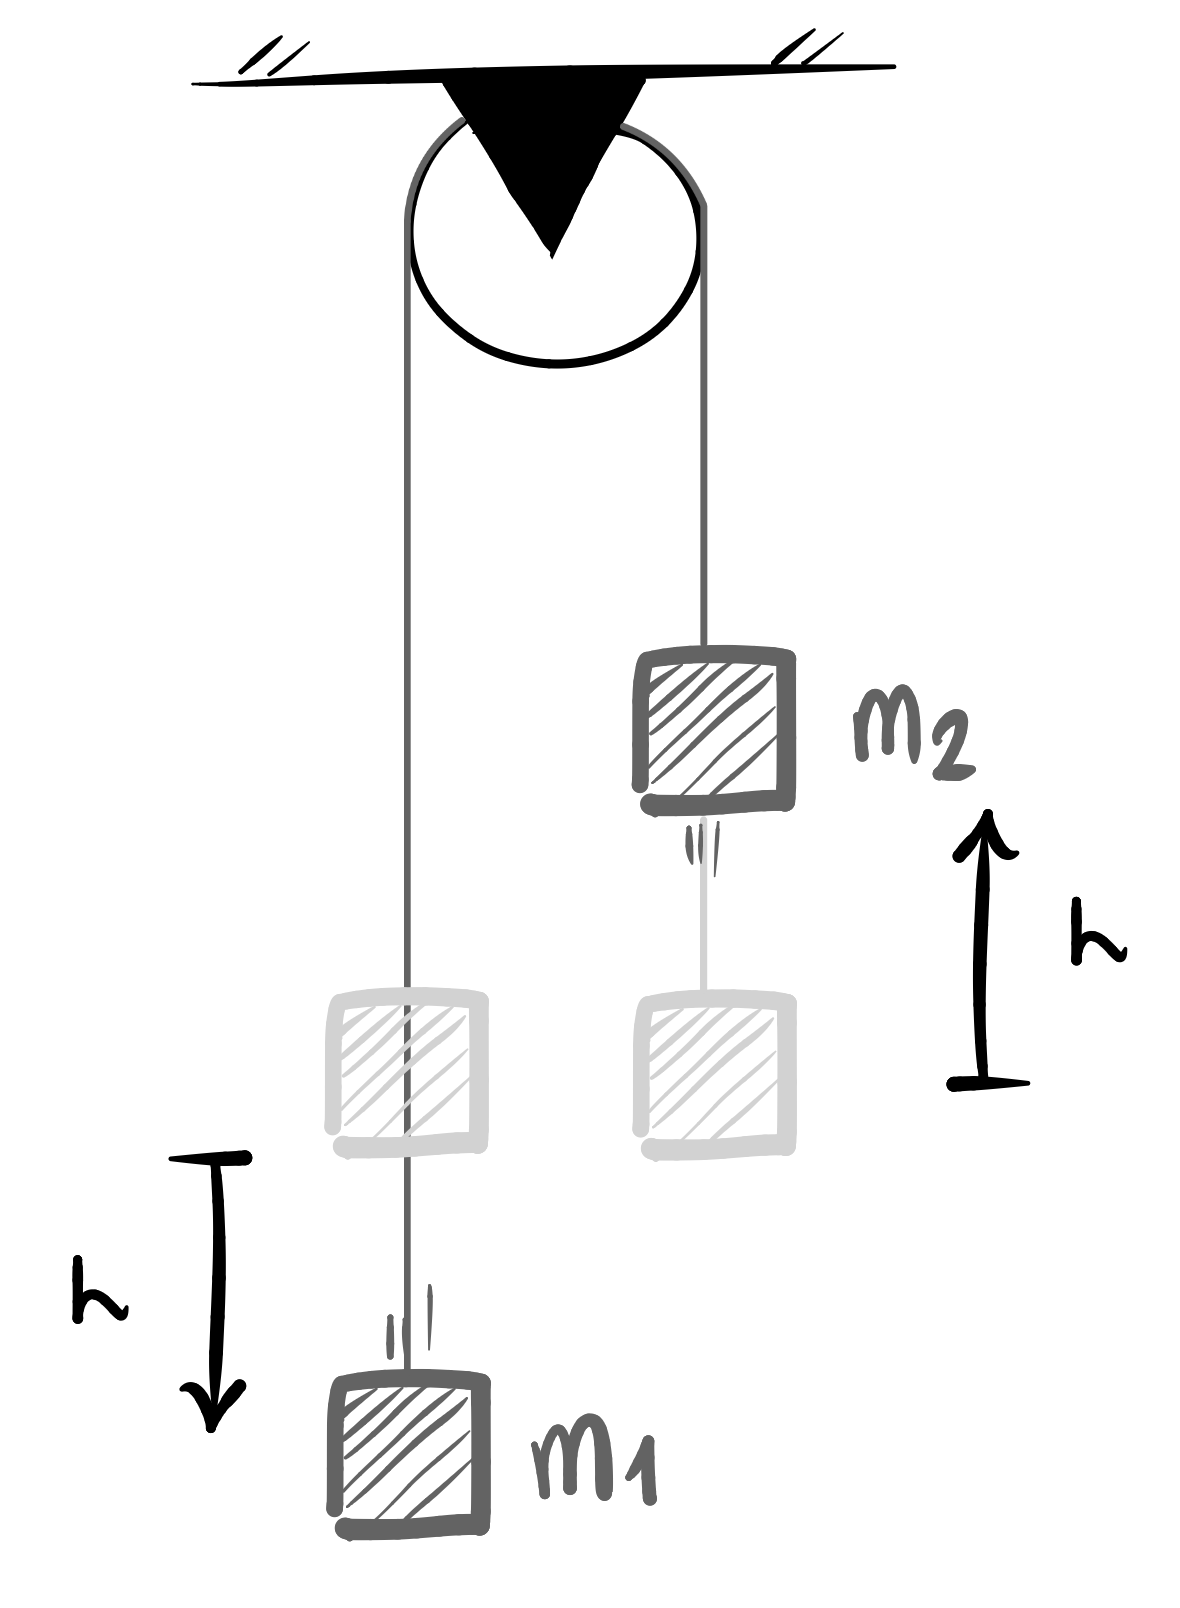
\includegraphics[width=0.3\linewidth]{imagensenergia/atwoodenergia.png}
\captionof{figure}{Análise energética da Máquina de Atwood.}
\label{fig_energia_atwoodenergia}
} 
\vspace{0.3cm}

Como o fio é inextensível, quando $m_1$ desce uma distância $h$,
$m_2$ sobe a mesma distância $h$, e ambos adquirem a mesma rapidez
$v$. A tração $T$ no fio realiza trabalhos sobre os dois blocos em
sentidos opostos:
\begin{align}
    W_{T,1} &= -T h \quad (\text{tração para cima, bloco desce}) \nonumber \\
    W_{T,2} &= +T h \quad (\text{tração para cima, bloco sobe}) \nonumber
\end{align}


\noindent Somando:

\[
  W_{T,1} + W_{T,2} = -Th + Th = 0.
\]

\noindent e os trabalhos das trações se cancelam. O único trabalho líquido sobre o
sistema é o do peso de cada bloco:

\[
  W_{P,1} = m_1 g h \quad (m_1 \text{ desce } h)
  \qquad \text{ e } \qquad
  W_{P,2} = -m_2 g h \quad (m_2 \text{ sobe } h).
\]

Perceba que, na descida, o peso está a favor do movimento, de modo que o trabalho é positivo ($\theta = 0^\circ \implies \cos \theta = 1$). Já na subida, o peso se opõe ao movimento, de modo que o trabalho é negativo ($\theta = 180^\circ \implies \cos \theta = -1$). O trabalho total da força peso neste sistema é, portanto:

$$ W = m_1gh - m_2gh = (m_1 - m_2)gh.$$


A variação de energia cinética do sistema (ambos partem do repouso) é:

\[
  \Delta E_c = \tfrac{1}{2}(m_1 + m_2)\,v^2.
\]

Aplicando o Teorema da Energia Cinética, teremos

\[
  W = \Delta E_c \implies(m_1 - m_2)gh = \tfrac{1}{2}(m_1 + m_2)\,v^2 \implies \boxed{v = \sqrt{\frac{2(m_1 - m_2)\,g\,h}{m_1 + m_2}}.}
\]



\noindent O resultado supõe $m_1 > m_2$, condição necessária para que
o sistema de fato se mova com $m_1$ descendo. Observe que $v$ cresce
com a diferença $m_1 - m_2$ e decresce com a soma $m_1 + m_2$ ---
o numerador mede o ``desequilíbrio'' gravitacional que impulsiona o
sistema; o denominador mede a inércia total que resiste à aceleração.
Tratar o sistema como um todo eliminou a necessidade de calcular $T$:
forças internas nunca aparecem no trabalho total do sistema,
princípio que reaparecerá em outros contextos.


\end{exemplo}


\vspace{0.3cm}





\begin{secnivel}[Energia Potencial Elástica]{I}{Energia Potencial Elástica}
 

  \eqLdois{dem}{eq_energia_potencialelastica}{E_\text{PE} = \dfrac{1}{2}kx^2}
  
\end{secnivel}





\secgfe{De onde vem}

Já calculamos o trabalho feito pela força elástica na seção em que definimos o trabalho -- convidamos o leitor a retornar ao cálculo feito com base na Figura \ref{fig_energia_trabalhoforcaelastica}. O resultado que obtivemos é que o trabalho feito pela força elástica ao levar a mola de um comprimento com deformação $x$ até o seu comprimento natural foi igual a $\sfrac{kx^2}{2}.$


Como a mola termina no seu comprimento natural, sua energia potencial elástica nessa posição é, naturalmente, zero. Logo, a variação de energia potencial elástica naquela situação é 

$$\Delta E_\text{P} = E_\text{P,f} - E_\text{P,i} = 0 - E_\text{P,i} = - E_\text{P,i},$$

\noindent em que $E_\text{P,i}$ é a energia potencial elástica inicial da mola, quando ela está no comprimento $x.$ Usando a Equação \eqref{eq_energia_trabalhoevariacaoenergiapotencial}, que define o conceito de energia potencial, somos levados a

 $$ W = -\Delta E_\text{P} \implies \dfrac{1}{2}kx^2 = - (- E_\text{P,i}) \implies E_\text{P,i} = \dfrac{1}{2}kx^2, $$

\noindent que é exatamente o que diz a Equação \eqref{eq_energia_potencialelastica}: quando deformada (comprimida ou esticada) de um tanto $x$, a energia potencial armazenada na mola é igual a $\sfrac{kx^2}{2}.$




\secgfe{Onde é usada}

A Equação \eqref{eq_energia_potencialelastica} aparece em qualquer situação em que uma mola (ou qualquer elemento
elástico) faça parte do sistema energético de um problema. Mas o leitor seria ingênuo em imaginar que isso se
restringe aos blocos e molas dos livros didáticos de Física. Molas estão em toda parte, frequentemente
disfarçadas.

A suspensão de um automóvel é, em essência, uma mola: ao passar por um buraco, a roda
comprime a mola e converte a energia do impacto em $E_\text{PE}$, que é então dissipada
gradualmente pelo amortecedor. O solado de um tênis de corrida de alta performance funciona
da mesma forma --- comprime ao tocar o solo e devolve parte da energia ao corredor no
passo seguinte, reduzindo o esforço muscular. O arco de um arqueiro armazena $E_\text{PE}$ ao
ser tensionado e a transfere integralmente à flecha ao ser solto: $\frac{1}{2}kx^2 =
\frac{1}{2}mv^2$. O trampolim, o estilingue e a catapulta de brinquedo operam pelo mesmo
princípio.

% Mais importante para o que vem a seguir: a Equação \eqref{eq_energia_potencialelastica} é um dos três termos da Lei
% de Conservação da Energia Mecânica, dada pela Equação \ref{}. Em qualquer sistema onde molas e
% gravidade atuem conjuntamente, a energia total se conserva entre as três formas:
% %
% \begin{equation*}
%     E_C + E_{PG} + E_{PE} = \text{constante},
% \end{equation*}
% %
% e é exatamente a Equação~(5.5) que quantifica a parcela elástica dessa soma. Veremos isso em mais detalhes em breve.





\secgfe{Erros comuns}

O erro mais comum é o leitor confundir a força elástica, dada por $F=kx$ -- a lei de Hooke --, com a energia potencial elástica, dada pela Equação \eqref{eq_energia_potencialelastica}. A primeira se refere à força feita por uma mola: ela é diretamente proporcional à deformação $x$ da mola. A segunda se refere ao trabalho que essa força realiza -- a energia que fica acumulada na mola -- quando se comprime a mola do seu estado natural até o estado de deformação $x.$

Outro erro comum é considerar o valor de $x$ como sendo o comprimento da mola, e não sua deformação. Considere, por exemplo, uma mola de comprimento natural $\ell_0 = 50 $cm e constante elástica $k=100$ N/m. Ao ser esticada até que seu comprimento seja $\ell= 60$cm, qual é a energia potencial elástica armazenada na mola?

É comum que o leitor considere o valor de $x$, na Equação \eqref{eq_energia_potencialelastica}, como sendo o valor do comprimento atual da mola, isto é, $x=60$cm. O valor de $x,$ contudo, é o quanto a mola está deformada, que neste caso vale $x=\Delta \ell = \ell - \ell_0 = 60 - 50 = 10 \text{cm} = 0.1 \text{m}$. Logo, a energia potencial elástica da mola nessa situação seria de 

$$ E_\text{PE} = \dfrac{1}{2} \cdot 100 \cdot (0.1)^2 = 0.5 \text{ J}.$$


\secgfe{Observações}

A Equação \eqref{eq_energia_potencialelastica} é simétrica em $x$: $E_\text{PE}(x) = E_\text{PE}(-x)$. Isso reflete o fato de
que a mola armazena a mesma quantidade de energia ao ser comprimida ou estendida de uma
mesma magnitude.  Naturalmente, em $x=0$ é o ponto de energia potencial nula:  $E_p = \frac{1}{2}k 0^2 = 0.$



% No gráfico $E_\text{PE} \times x$, isso se manifesta como uma parábola com
% vértice em $x = 0$ --- a posição de equilíbrio, onde a energia potencial é mínima (e nula,
% por convenção). A Figura \ref{} ilustra tal gráfico.



Tal escolha de referência --- $E_\text{P} = 0$ quando $x = 0$ --- é a mais natural, mas não
é obrigatória. Assim como na energia potencial gravitacional escolhemos livremente o nível
de referência $h = 0$, poderíamos em princípio definir $E_{PE} = 0$ em qualquer posição.
O que nunca muda, e é por isso fisicamente relevante, é a \textit{variação} de energia
potencial $\Delta E_\text{PE}$ entre dois estados --- não o valor absoluto de $E_\text{PE}$ em um
único estado.

Por fim, convém comparar as duas energias potenciais que o leitor agora conhece:
%

\begin{align}
      E_\text{PG} &= mgh \qquad \text{(linear em } h\text{)} \nonumber \\
      E_\text{PE} &= \tfrac{1}{2}kx^2 \qquad \text{(quadrática em } x\text{)} \nonumber
\end{align}


% É interessante notar o contraste. A força gravitacional (peso) é constante na superfície da Terra: $P = mg$,
% independentemente da altura. O gráfico $F \times h$ é um retângulo, cuja área --- o trabalho
% --- é $mgh$. Já a força elástica cresce linearmente com a deformação: $F = kx$. O gráfico
% $F \times x$ é um triângulo, cuja área é $\frac{1}{2}kx^2$. A forma da energia potencial é,
% em cada caso, a área sob o respectivo gráfico da força --- um resultado que unifica as duas
% equações num mesmo raciocínio geométrico.

A força gravitacional (o peso do corpo) é dado por $P = mg$. Trata-se de uma força \textit{constante}: não importa se o corpo está a 1~m ou a 10~m do chão, a força gravitacional que age sobre ele é a mesma. Ao elevarmos o corpo de
uma altura $h$, trabalhamos sempre contra a mesma força $mg$, de modo que o trabalho
realizado cresce proporcionalmente à altura: dobramos a altura, dobramos o trabalho,
dobramos a energia armazenada. Daí o comportamento linear: $E_\text{PG} \propto h$.

Já a força elástica, dada por $F = kx$, por sua vez, é uma força \textit{variável}: quanto mais
deformamos a mola, maior é a força que ela nos impõe. Ao comprimir a mola de $x_0$,
não trabalhamos contra uma força constante --- trabalhamos contra uma força que começa
em zero e vai crescendo até $kx_0$. No início, a mola quase não resiste; no final, ela
resiste com força máxima. O trabalho acumulado ao longo desse processo não é simplesmente
$F \cdot x_0$ (pois não há uma única força $F$), mas sim $\frac{1}{2}kx_0^2$. Portanto, ao dobrar a altura $h$, a energia potencial gravitacional dobra; mas ao dobrar a deformação $x$ da mola, a energia potencial elástica quadruplica. O fator quadrático na Equação \eqref{eq_energia_potencialelastica} captura o fato de que a força elástica aumenta com a deformação, mostrando que é mais difícil empurrar a mola quanto mais deformada ela está e, portanto, a energia potencial armazenada na mola cresce em uma taxa mais acelerada do que no caso gravitacional.


Esse raciocínio é geral: a forma da energia potencial associada a qualquer força
conservativa $F(x)$ é sempre a área sob o gráfico dessa força. Para uma força constante, essa área é um retângulo, e a energia é linear na posição. Para uma força linear (como a elástica), essa área é um triângulo, e a energia
é quadrática. Para forças mais complexas, surgem expressões mais elaboradas ---
mas o princípio é sempre o mesmo: \textit{a forma da energia potencial dependerá de como varia a força}.


\vspace{0.3cm}

\begin{exemplo}[Nível I]\label{exemplo_energia_potencialelasticaex01}

Duas molas, $A$ e $B$, têm constantes elásticas $k_A = 200\ \text{N/m}$ e
$k_B = 800\ \text{N/m}$. Ambas são comprimidas da mesma deformação $x = 5\ \text{cm}$.
Qual das duas armazena mais energia, e por quê?

\resolucao

Calculando $E_{PE}$ para cada mola:
%
\begin{align*}
    E_\text{PE,A} &= \frac{1}{2} \cdot 200 \cdot (0{,}05)^2 = 0{,}25\ \text{J}, \\
    E_\text{PE,B} &= \frac{1}{2} \cdot 800 \cdot (0{,}05)^2 = 1{,}00\ \text{J}.
\end{align*}

A mola $B$ armazena quatro vezes mais energia, pois sua constante $k$ é quatro
vezes maior. Como a deformação é a mesma nas duas, a energia é diretamente
proporcional a $k$: uma mola mais rígida resiste mais ao longo de toda a
compressão e, portanto, acumula mais energia para a mesma deformação.


\end{exemplo}


\vspace{0.3cm}





\begin{exemplo}[Nível II]\label{exemplo_energia_potencialelasticaex02}

Um bloco de massa $m = 0{,}4\ \text{kg}$ é lançado sobre uma superfície
horizontal sem atrito e comprime uma mola de constante $k = 1000\ \text{N/m}$ de
$x_0 = 8\ \text{cm}$. Qual era a velocidade do bloco no instante em que tocou a mola?

\resolucao

No instante do contato, o bloco possui energia cinética
$E_\text{C} = \frac{1}{2}mv^2$ e a mola está relaxada ($E_\text{PE} = 0$). Na compressão máxima,
o bloco para ($E_\text{C} = 0$) e toda a energia cinética foi convertida em $E_\text{PE}$. Pelo
Teorema da Energia Cinética, o trabalho total realizado sobre o bloco ao longo do
percurso de comprimento $x_0$ é:
%
\begin{equation*}
    W_{\text{elást}} = \Delta E_\text{C} \implies
    -\frac{1}{2}kx_0^2 = 0 - \frac{1}{2}mv^2 \implies
    v = x_0\sqrt{\frac{k}{m}},
\end{equation*}

\noindent que, substituindo os valores, nos leva a $v= 4$ m/s.

Pela simetria do problema --- superfície lisa, mola ideal --- o bloco sairá da mola
com exatamente a mesma velocidade de $4{,}0\ \text{m/s}$, porém no sentido contrário.

\end{exemplo}


\vspace{0.3cm}





\begin{exemplo}[Nível III]\label{exemplo_energia_potencialelasticaex03}

Um bloco de massa $m = 1\ \text{kg}$ é lançado com velocidade $v_0 = 4\ \text{m/s}$
sobre uma superfície horizontal sem atrito em direção a uma mola de constante
$k = 200\ \text{N/m}$ fixada a uma parede. A mola está inicialmente relaxada. Determine: 

\begin{itemize}
    \item [a)] a compressão máxima $x_0$;

    \item [b)] a velocidade do bloco quando a mola estiver comprimida de exatamente $x_0/2$.
\end{itemize}

\resolucao

\textit{a)} Na compressão máxima, o bloco está momentaneamente em repouso: $v = 0$.
Pelo Teorema da Energia Cinética, o trabalho realizado pela força elástica ao longo
do percurso de comprimento $x_0$ é:
%
\begin{equation*}
    W_{\text{elást}} = \Delta E_C \implies
    -\frac{1}{2}kx_0^2 = 0 - \frac{1}{2}mv_0^2,
\end{equation*}

\noindent de onde segue que

$$ x_0 = v_0\sqrt{\frac{m}{k}} = 4 \cdot \sqrt{\frac{1}{200}}
    \approx \frac{4}{14{,}14} \approx 0{,}283\ \text{m} \approx 28{,}3\ \text{cm}.$$

\textit{b)} Agora aplicamos o Teorema da Energia Cinética ao percurso que vai do
instante inicial (mola relaxada, velocidade $v_0$) até o instante em que a compressão
é $x_0/2$ (velocidade $v$, desconhecida). O trabalho da força elástica ao longo desse
percurso é:
%
\begin{equation*}
    W_{\text{elást}} = -\frac{1}{2}k\left(\frac{x_0}{2}\right)^2
    = -\frac{1}{2} \cdot 200 \cdot \left(\dfrac{0,2830}{2} \right)^2 \approx -2{,}0\ \text{J}.
\end{equation*}

Pelo Teorema da Energia Cinética:
%
\begin{equation*}
    -2{,}0 = \frac{1}{2} \cdot 1 \cdot v^2 - \frac{1}{2} \cdot 1 \cdot 16
    \implies v^2 = 16 - 4{,}0 = 12{,}0
    \implies v \approx 3{,}46\ \text{m/s}.
\end{equation*}

O resultado merece uma observação: quando a mola está comprimida à metade ($x_0/2$),
o bloco ainda possui $3/4$ da energia cinética inicial --- não metade. Isso ocorre
porque $E_\text{PE} \propto x^2$: comprimir a mola à metade da deformação máxima armazena
apenas $1/4$ da energia máxima, deixando os outros $3/4$ como energia cinética. A
mola resiste de forma crescente --- devagar no início, cada vez mais depressa ao
final ---  e é exatamente por isso que a Equação \eqref{eq_energia_potencialelastica} leva um expoente quadrático.
\end{exemplo}













\begin{secnivel}[Conservação da Energia Mecânica]{I}{Lei de Conservação da Energia Mecânica}


  \eqLdois{dem}{eq_energia_conservacaodaenergiamecanica}{\Delta E_\text{M} =0}
  
\end{secnivel}

A Equação \eqref{eq_energia_conservacaodaenergiamecanica} diz que, sob a ação exclusivamente de forças conservativas, a energia mecânica $E_\text{M}$ de um sistema se conserva, isto é, ela não varia.





\secgfe{De onde vem}

Enfim, chegamos aonde queríamos: o princípio mais importante de todo o capítulo -- e a razão de termos construído tudo o que foi feito até aqui.

Depois de todo o laborioso trabalho de construção feito até aqui, demonstrar a Equação \eqref{eq_energia_conservacaodaenergiamecanica} é quase automático. Nós definimos a energia mecânica $E_\text{M}$ de uma partícula (ou de um sistema de partículas) como sendo a soma da sua energia cinética com suas energias potenciais:

$$ E_\text{M} = E_\text{C}  + E_\text{P},$$

\noindent em que, no termo $E_P$ entra todos os tipos de energias potenciais envolvidas no contexto: energia potencial gravitacional, potencial elástica, potencial elétrica.

Logo, aplicando a variação, teríamos

$$ \Delta E_\text{M} = \Delta E_\text{C}  + \Delta E_\text{P}.$$

Contudo, o Teorema da Energia Cinética nos diz que $\Delta E_\text{C}=W,$ em que $W$ é o trabalho da resultante das forças que atuam na partícula. Já a definição de energia potencial, dada pela Equação \eqref{eq_energia_trabalhoevariacaoenergiapotencial}, nos diz que $W_\text{FC} = - \Delta E_\text{P},$ em que $W_\text{FC}$ representa o trabalho das forças conservativas. Se atuarem apenas forças conservativas no corpo, então o trabalho total será oriundo apenas de forças conservativas, isto é: $W = W_\text{FC} $ e, desse modo, teríamos  

$$W = \Delta E_\text{C} = -\Delta E_\text{P} \implies \Delta E_\text{C} + \Delta E_\text{P} = 0,$$

\noindent ou seja, a variação da energia mecânica $E_\text{M} = E_\text{C}  + E_\text{P}$ é nula, como constata a Equação \eqref{eq_energia_conservacaodaenergiamecanica}.

Considere, a título de ilustração, a situação da Figura \ref{fig_energia_conservacaodaenergia}, em que uma bola é abandonada \emph{do repouso} em cima de uma rampa. Atritos e resistência do ar são desprezíveis. Tomando como nível zero de energia potencial gravitacional ($h=0)$ sendo o solo, digamos que a bolinha tem massa $m= 2$kg e é abandonada da altura inicial $h_0 = 6$m. Desse modo, sua energia mecânica inicial é

$$ E_\text{M} =  E_\text{P} +  E_\text{C} = mg h_0 + \dfrac{m\cancelto{0}{v^2}}{2} = 2 \cdot 10 \cdot 6 = 120 \text{ J.}$$

O que a Equação \eqref{eq_energia_conservacaodaenergiamecanica} diz é que, havendo apenas forças conservativas realizando trabalho, o valor da energia mecânica da partícula será, em qualquer instante, os mesmos 120 J.


\vspace{0.3cm}
{
\centering
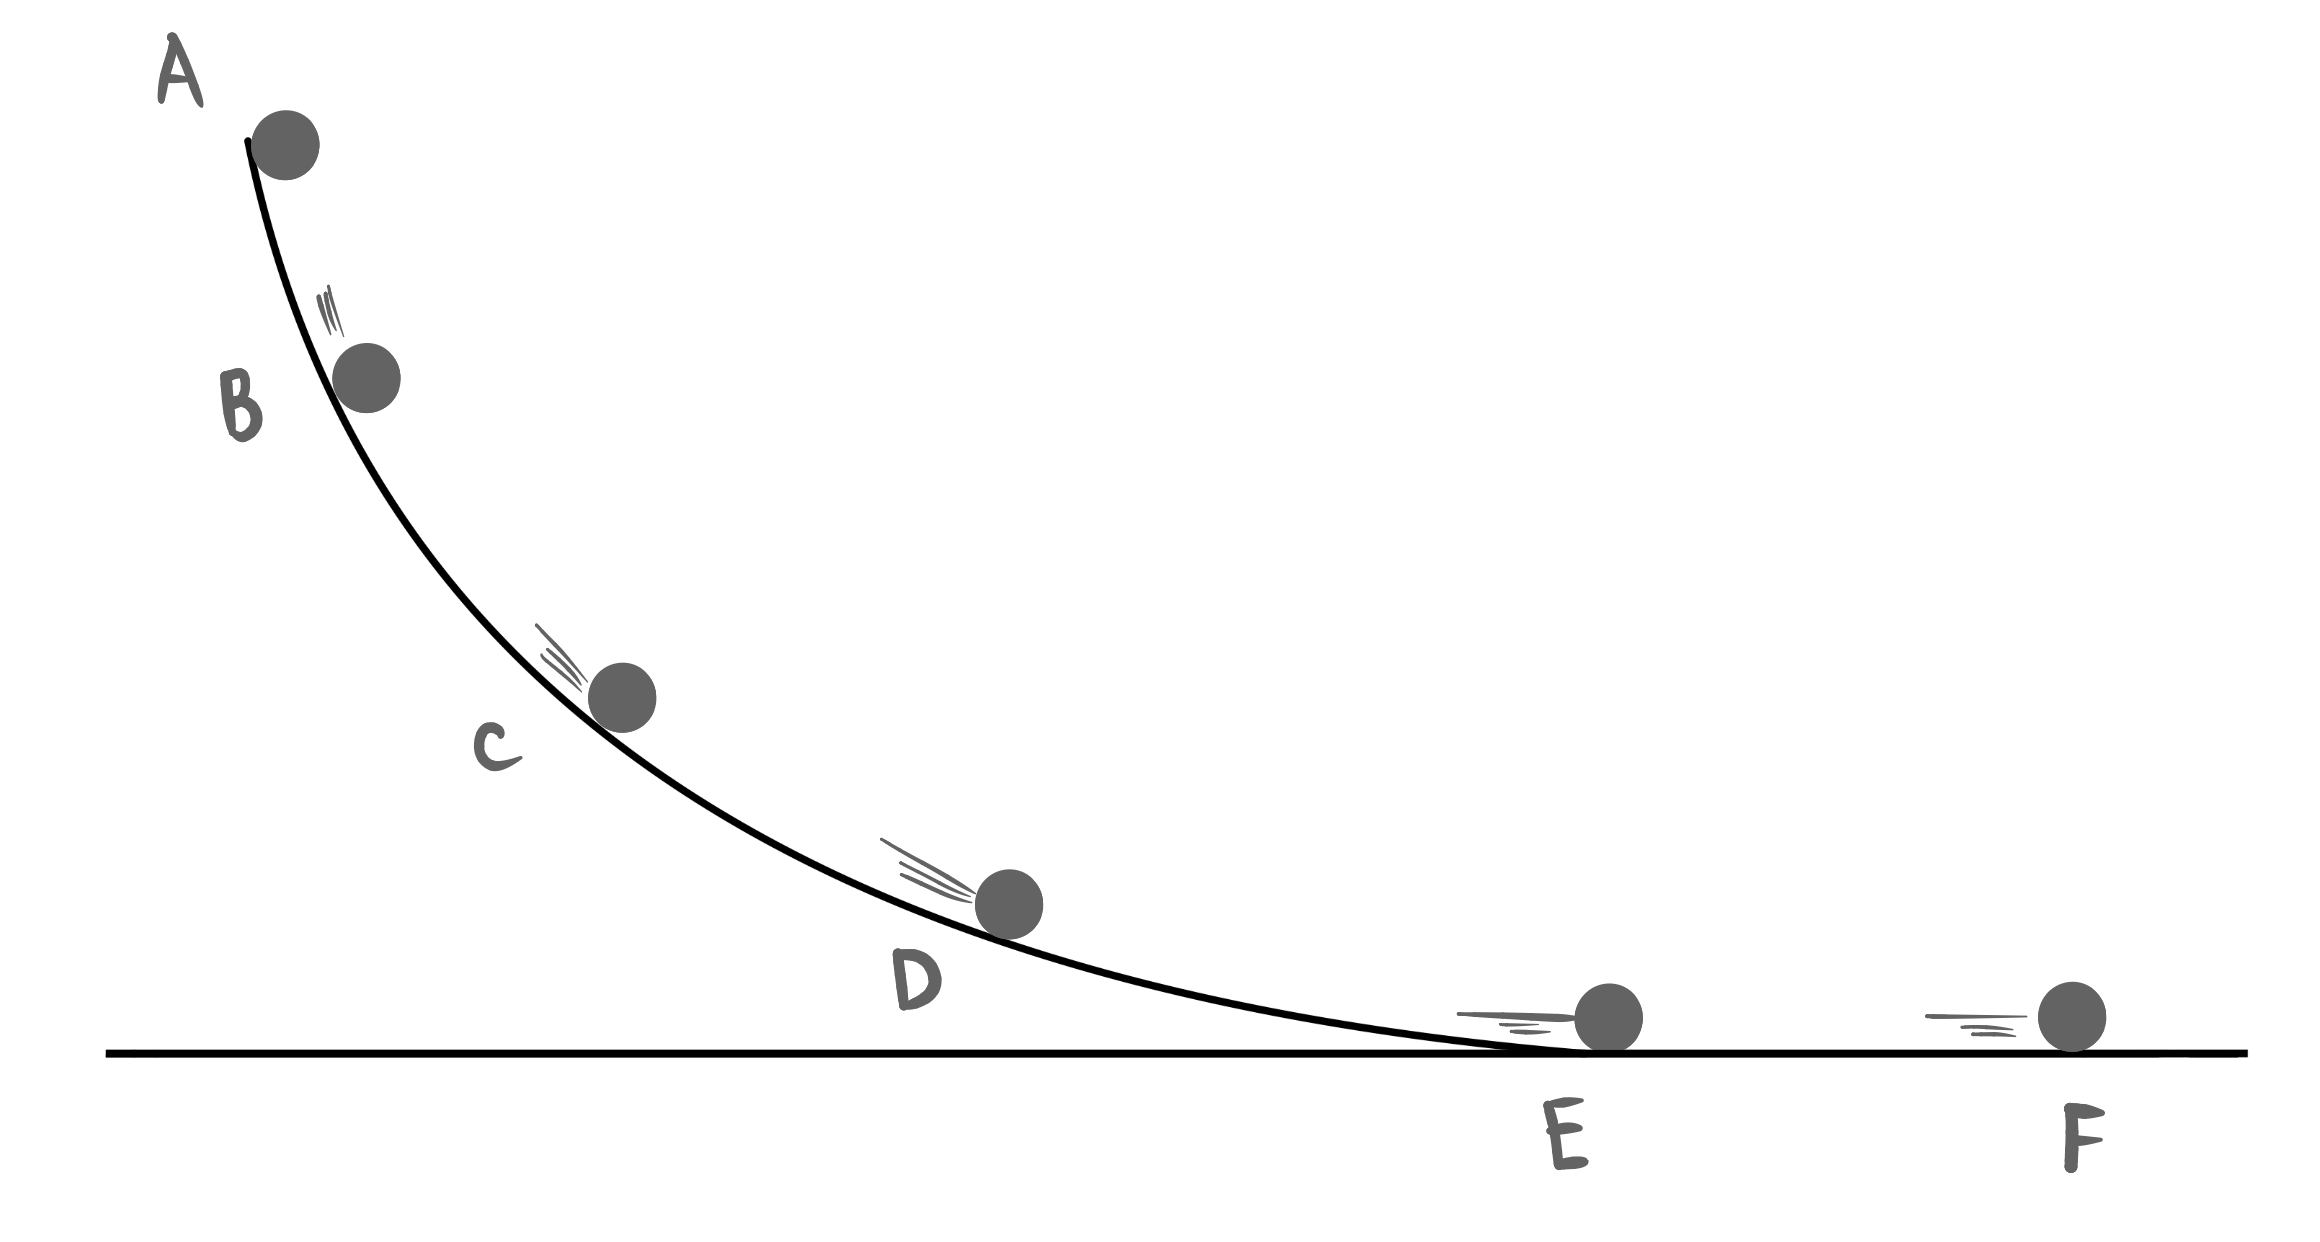
\includegraphics[width=0.5\linewidth]{imagensenergia/conservacaodaenergia.png}
\captionof{figure}{Bola escorregando na rampa sem atrito.}
\label{fig_energia_conservacaodaenergia}
} 
\vspace{0.3cm}

Sendo assim, é possível usar esta constante para interpretar e estudar o movimento. Na posição inicial a energia é puramente potencial gravitacional. Já na posição $B$ a partícula caiu um pouco, de modo que perdeu um pouco de energia potencial gravitacional. Porém, para satisfazer a Equação \eqref{eq_energia_conservacaodaenergiamecanica}, ela precisa ter ganhado exatamente o mesmo tanto de energia cinética. 

A tabela abaixo destaca os valores de energia potencial, cinética e mecânica (em joules) para os diferentes estágios do movimento. Note que o que ocorre é apenas um processo de \emph{conversão} de um tipo de energia (potencial) em outro (cinética), haja vista que a soma das duas é sempre constante. Nos pontos $E$ e $F$ a partícula atingiu o nível zero de energia potencial: agora ela é zero, e toda a energia foi convertida em cinética.

\[
\begin{array}{c|c|c|c}
\hline
\text{Posição} & E_c & E_p & E_m = E_p + E_c \\
\hline
A & 0   & 120 & 120 \\
\hline
B & 20  & 100 & 120 \\
\hline
C & 70  & 50  & 120 \\
\hline
D & 100 & 20  & 120 \\
\hline
E & 120 & 0   & 120 \\
\hline
F & 120 & 0   & 120 \\
\hline
\end{array}
\]


Note que, ao fazer uma variação entre dois pontos quaisquer de um tipo de energia, ela será exatamente compensada pela variação do outro tipo de energia. Por exemplo, avaliando entre os pontos $A$ e $D$, teríamos:

\begin{align}
    \Delta E_C &= 100 - 0 = 100 \text{J} \nonumber \\
    \Delta E_P &= 120 - 20 = -100 \text{J}, \nonumber 
\end{align}


\noindent de modo que o ganho de energia cinética (+100) é exatamente igual à perda de energia potencial (-100), o que é o equilíbrio exato necessário para que a energia mecânica se conserve. É por isso que a Equação \eqref{eq_energia_trabalhoevariacaoenergiapotencial} -- que define o conceito de energia potencial -- possui um sinal negativo: a variação da energia potencial terá sempre o sinal contrário da variação da energia cinética, uma vez que quando uma aumenta a outra diminui, e vice-versa.

Avaliando, por exemplo, entre os pontos $D$ (considerado aqui como ponto inicial) e $B$ (considerado aqui como ponto final), teríamos:

\begin{align}
    \Delta E_C &= 20 - 100 = -80 \text{J} \nonumber \\
    \Delta E_P &= 100 - 20 = 80 \text{J}, \nonumber 
\end{align}

\noindent e, novamente, a diminuição de energia cinética é exatamente igual -- em módulo -- ao aumento da energia potencial, sendo o sinal oposto o responsável pelo significado de que o aumento de uma energia é compensado pela diminuição da outra, de modo que suas variações terão sempre sinais contrários, o que faz com que sua soma dê sempre zero.

\secgfe{Onde é usada}

A Equação \eqref{eq_energia_conservacaodaenergiamecanica} é, sem exagero, a ferramenta mais poderosa desta seção --- e uma
das mais versáteis de toda a mecânica. Ela transforma em problemas
elementares situações que seriam intratáveis pela análise por leis de Newton.

Para ilustrar isso, veja o exemplo do lançamento do projétil. Considere uma pedra de massa $m = 0{,}3$
kg lançada de uma altura $h = 10$ m com velocidade $v_0 = 8$ m/s, em um ângulo
qualquer com a horizontal. Pergunta: qual é a velocidade da pedra quando ela estiver
a $h' = 5$ m do solo? Pela Segunda Lei de Newton, seria necessário decompor $v_0$ em
componentes horizontal e vertical, tratar as duas direções com equações separadas e
depois recombinar --- e o resultado dependeria do ângulo de lançamento. Pela
conservação da energia, basta escrever um único balanço entre a posição inicial e a
posição final, isto é a, a conservação da energia mecânica: $E_{\text{M}_i} = E_{\text{M}_f}.$ Abrindo esse cálculo, teremos:

\begin{align}
    E_{\text{C}_i} + E_{\text{P}_i} &=  E_{\text{C}_f} + E_{\text{P}_f} \nonumber \\
     \frac{1}{2} \cancel mv_0^2 + \cancel mgh &= \frac{1}{2} \cancel mv^2 + \cancel mgh'. \nonumber
\end{align}
%

Desenvolvendo, teremos

\begin{equation*}
    \frac{1}{2}v^2 = \frac{1}{2}v_0^2 + g(h - h')
    = \frac{1}{2}(64) + 10 \cdot (10 - 5) = 32 + 50 = 82\ \text{J/kg}
\end{equation*}
%
\begin{equation*}
    v = \sqrt{2 \cdot 82} \approx 12{,}8\ \text{m/s.}
\end{equation*}

Três observações merecem destaque. Primeiro: a massa cancelou --- o resultado
independe de $m$. Segundo: o ângulo de lançamento não apareceu em lugar algum ---
qualquer ângulo que produza $v_0 = 8$ m/s leva ao mesmo resultado, o que seria
completamente obscuro na abordagem vetorial. Terceiro: a posição intermediária entre
$h$ e $h'$ --- a trajetória percorrida, os valores de velocidade ao longo do caminho
--- foi completamente irrelevante para o cálculo.

Além do projétil, a Equação \eqref{eq_energia_conservacaodaenergiamecanica} é o instrumento central em toda situação em que haja troca entre as formas de energia mecânica: pêndulos, montanhas-russas, blocos
em planos inclinados, sistemas mola-bloco, saltos, etc.
Em todos esses casos, o que muda é apenas quais parcelas de $E_M$ são relevantes
em cada instante --- mas a soma se conserva\footnote{Na mecânica quântica, descobriu-se que partículas minúsculas --- como elétrons --- simplesmente não possuem uma trajetória bem definida. Não é uma limitação dos nossos instrumentos: a natureza, nessa escala, recusa-se a fornecer uma. E sem trajetória, a segunda lei de Newton perde completamente o sentido --- afinal, $\vec{F} = m\vec{a}$ é uma equação \textit{sobre o movimento}, sobre como a posição muda instante a instante. A energia, porém, sobrevive à reviravolta. Perguntar ``quanta energia esse sistema possui?'' continua sendo uma pergunta perfeitamente legítima --- mesmo quando ``onde está essa partícula agora?'' já não é. Não por acaso, a equação fundamental da mecânica quântica, proposta por Schrödinger em 1926, é inteiramente construída ao redor da energia do sistema, e não das forças que atual nele. Newton saiu; a energia ficou. Eis mais um aspecto que revela a riqueza e profundidade da descrição escalar da dinâmica: a física quântica é toda escrita em termos dessa formulação.}.



\secgfe{Erros comuns}

Os principais erros aqui são:

\begin{enumerate}
    \item [(i)] Usar a Equação \eqref{eq_energia_conservacaodaenergiamecanica} quando atuam forças dissipativas.

    Neste caso, a energia mecânica não se conserva, e isso precisa ser levado em consideração. Considere, por exemplo, um bloco de \SI{2{,}0}{kg}, que é abandonado do repouso
no topo de uma rampa e desliza até o chão, descendo uma altura de
\SI{4{,}0}{m}. Ao longo do percurso, a força de atrito realiza um
trabalho de módulo \SI{24}{J} sobre o bloco.  Qual é a velocidade do bloco ao chegar à base da rampa?

O primeiro impulso de muitos estudantes é aplicar a lei de conservação
da energia mecânica --- e aqui está exatamente o ponto que este exemplo
quer iluminar: \emph{ela não vale quando há atrito}.

A conservação da energia mecânica

\[
  E_{\text{M}_i} = E_{\text{M}_f}
\]

\noindent só é válida quando \emph{todas} as forças que atuam sobre o
sistema são conservativas (força peso, elástica, elétrica) ou, caso haja outras forças, elas sejam do tipo que não realizam trabalho (tração, normal). Já o atrito cinético é
uma força dissipativa: ele realiza trabalho, mas não é conservativo. Ele converte parte da energia mecânica em energia
térmica --- em calor, perceptível no aquecimento das superfícies em
contato. Essa energia não desaparece do universo, mas escapa do sistema
mecânico de forma irrecuperável.

A equação correta, portanto, é a seguinte: a energia mecânica
\emph{inicial} é igual à energia mecânica \emph{final} mais a energia
dissipada pelo atrito:

\begin{equation}
  \boxed{E_{\text{M}_i} = E_{\text{M}_f} + |W_{\text{Fat}}|} \nonumber
\end{equation}

\noindent A parcela $|W_{\text{Fat}}|$ representa justamente o quanto
de energia mecânica foi ``roubado'' pelo atrito e entregue ao ambiente
na forma de calor. O leitor pode imaginar a equação acima como um
balanço financeiro: a quantia inicial menos o que foi gasto é igual à
quantia que sobrou.

Desenvolvendo, vemos que o bloco parte do repouso ($v_i = 0$) numa altura
$h = \SI{4{,}0}{m}$, e chega à base, que tomamos como referência de
energia potencial ($h_f = 0$). Portanto:

\[
  E_{\text{M}_i} = E_{\text{P}_i} + E_{\text{C}_i}  = mgh + 0 = 2 \cdot 10 \cdot 4
  = \SI{80}{J}.
\]

\[
  E_{\text{M}_f} = E_{\text{P}_f} + E_{\text{C}_f}  = 0 + \dfrac{1}{2}mv_f^2
  = \dfrac{1}{2} \cdot 2 \cdot \,v_f^2 = v_f^2 \;\text{(em joules).}
\]

Substituindo na equação de balanço:

\[
  E_{\text{M}_i} = E_{\text{M}_f} + |W_{\text{Fat}}| \implies 80 = v_f^2 + 24,
\]

\noindent de onde segue que 

 $$v_f = \sqrt{56} \approx \SI{7{,}5}{m/s}.$$


Note que, sem o atrito, a velocidade seria $v_f = \sqrt{80}
\approx \SI{8{,}9}{m/s}$. O atrito custou ao bloco 
\SI{24}{J}, reduzindo a velocidade
final. Esse contraste é uma boa verificação qualitativa: o resultado
com atrito \emph{deve} ser sempre menor do que o resultado sem atrito,
e o leitor deve suspeitar de qualquer conta que inverta essa ordem.

De forma mais analítica e para um caso geral, podemos escrever -- pelo Teorema da Energia Cinética -- que

$$ W_{\text{F}_R} = \Delta E_C \implies W_{\text{F}_{C}} + W_{\text{F}_{NC}} = \Delta E_C,  $$

\noindent em que quebramos o trabalho da força resultante $W_{\text{F}_R}$ em duas parcelas: o trabalho das forças conservativas, $W_{\text{F}_{C}}$, e o trabalho das forças não conservativas, $W_{\text{F}_{NC}}$. Ora, pela definição de energia potencial, sabemos que $W_{\text{F}_{C}} = - \Delta E_P,$ o que, na relação acima, produz:

$$ -\Delta E_P + W_{\text{F}_{NC}} = \Delta E_C,  $$

\noindent ou seja:

$$ \Delta E_C + \Delta E_P = W_{\text{F}_{NC}} \implies \boxed{\Delta E_M = W_{\text{F}_{NC}}.} $$

Essa pode ser vista como uma versão \emph{estendida} da Equação \eqref{eq_energia_conservacaodaenergiamecanica}: se o sistema está sob a ação exclusiva de forças conservativas\footnote{Ou, ainda que haja forças não conservativas, essas não realizem trabalho líquido.}, então $W_{\text{F}_{NC}} =0$ e a equação se reduz à lei de conservação da energia mecânica: $\Delta E_M = 0.$

Contudo, caso forças não conservativas atuem no sistema e realizem trabalho, a relação acima evidencia que o papel dessas forças é, justamente, variar a energia mecânica do sistema, como foi no caso da força de atrito.


    \item [(ii)] Trocar o referencial de energia potencial no meio da
conta.

Numa questão com rampa, o aluno define o chão como
nível de referência ($h = 0$) no estado inicial. Ao escrever o estado
final, esquece essa escolha e passa a medir a altura a partir de outro
ponto --- a base da rampa, o topo, ou qualquer outro que pareça mais
conveniente naquele momento.

A energia potencial gravitacional
$E_p = mgh$ só faz sentido \emph{em relação a um referencial fixo}.
O valor absoluto de $E_p$ não tem significado físico isolado; o que
importa é a \emph{diferença} $\Delta E_p$. Se o referencial muda no
meio do problema, essa diferença é calculada entre duas grandezas que
não se referem ao mesmo zero, e o resultado é simplesmente incorreto.

Portanto, escolha o referencial \emph{antes} de escrever
qualquer equação e mantenha-o até o fim. A escolha em si é livre ---
pode ser o chão, o ponto mais baixo da trajetória, qualquer nível
horizontal fixo --- mas deve ser \emph{única e explícita}. 

 \item [(iii)] Concluir que ``energia se conserva'' implica ``velocidade
se conserva''.

Um projétil é lançado e o aluno, sabendo que a
energia mecânica se conserva ao longo da trajetória (sem atrito),
conclui que a velocidade no ponto mais alto é a mesma que na largada.

Conservar energia mecânica significa que a
\emph{soma} $E_c + E_p$ permanece constante --- não cada parcela
individualmente. À medida que o projétil sobe, $E_p = mgh$ aumenta, e
portanto $E_c = \frac{1}{2}mv^2$ diminui: o projétil \emph{desacelera}.
Energia e velocidade são grandezas distintas; conservar a primeira não
congela a segunda.

Em qualquer ponto da trajetória, use

\[
  \tfrac{1}{2}mv_i^2 + mgh_i = \tfrac{1}{2}mv_f^2 + mgh_f
\]

\noindent para calcular a velocidade \emph{naquele ponto específico},
sempre considerando a altura correspondente. A velocidade só seria a
mesma em dois pontos distintos se esses pontos estivessem exatamente
à mesma altura --- o leitor consegue ver isso?

\item [(iv)] Tentar usar trabalho e energia para resolver problemas que envolvem informações temporais.

Como o leitor pode verificar, os conceitos de energia cinética, trabalho, energia potencial ou energia mecânica são conceitos que \emph{não trazem informações temporais}. A conservação da energia mecânica garante que, sob certas condições, um certo número -- a energia mecânica de uma partícula ou de um sistema -- é sempre o mesmo ao longo do processo. Porém, não diz nada sobre quanto de energia é cinética ou potencial em cada instante de tempo. É uma linguagem de conservação, não uma descrição temporal. Assim, problemas em que o objetivo é computar o tempo que leva para um processo ocorrer não podem ser resolvidos por essa linguagem -- eles devem ser abordados usando a \emph{descrição vetorial da dinâmica}: as Leis de Newton.

É comum, portanto, que algum leitor insista em tentar resolver problemas deste tipo por meio de trabalho e energia -- o que não é possível, como espero ter ficado claro com esta conversa.


\end{enumerate}




\secgfe{Observações}

% Essa seção será um breve digressão sobre a razão de termos construído todos os conceitos existentes neste capítulo. Caso o leitor esteja convencido e confortável com tudo o que foi feito até aqui -- e suas razões de fazê-lo --, sua leitura pode ser pulada, sem nenhum medo de se perder qualquer aspecto novo do conteúdo. Contudo, ao leitor mais curioso, essa seção deixará evidente qual é a principal diferença entre a formulação vetorial e a formulação escalar da dinâmica, além de deixar claro por qual razão criamos todos esses conceitos de trabalho-energia.
Esta seção é uma dessas pausas em que o autor, desconfiado de si mesmo, volta-se ao leitor e pergunta, quase em voz baixa: \emph{“Sabeis bem por que viemos até aqui?”}

Se o leitor, firme e satisfeito, já se sente em boa companhia com os conceitos apresentados — e, sobretudo, com as razões que os trouxeram à existência —, pode avançar sem peso na consciência. Não perderá fio algum da meada. Vá, pois, como cavaleiro seguro de seu caminho.

Mas, se há nele uma curiosidade mais inquieta — dessas que não se contentam com o resultado, mas exigem o porquê das coisas —, então que permaneça. Esta breve digressão lhe revelará, com alguma clareza, a diferença capital entre duas maneiras de contar a mesma história da dinâmica: a formulação vetorial, direta e fiel às forças, e a formulação escalar, mais econômica, quase astuta, que olha só para o estado inicial e final de um sistema, ignorando por completo o que se passa na \emph{travessia.}

Nessa digressão, deixaremos claro que não erguemos esses conceitos de trabalho e energia por capricho ou gosto de abstração, mas como quem forja uma nova ferramenta: para facilitar um certo trabalho, ou, pelo menos, para economizar \emph{energia} em sua execução.

Veja as duas situações da Figura \ref{fig_energia_newtonvsleibniz1}. Nas duas, solta-se uma bola de massa $m$, do repouso, de uma altura $h$ do solo. O problema é -- desprezando os atritos -- encontrar a velocidade da bola ao terminar de descer a rampa. Na primeira imagem temos um plano inclinado. Neste caso, as leis de Newton nos permitiriam resolver com facilidade do problema: a Equação \eqref{eq_dinamicanewtoniana_gsintheta} nos fornece a aceleração da massa no plano inclinado, que, sendo constante, nos possibilita usar as equações do MUV. Pela Equação de Torricelli, teríamos:

$$ v^2 = \cancelto{0}{v_0^2} + 2 a d \implies v^2 = 2 \cdot g \sin \theta \cdot d,$$

\noindent e, como $\sin \theta = \sfrac{h}{d},$ teremos

$$ v^2 = 2 \cdot g \cdot \dfrac{h}{\cancel d} \cdot \cancel d \implies \boxed{v = \sqrt {2gh},}$$

\noindent de modo que a solução sai de forma simples: conhecendo a altura $h$ em que a bola foi abandonada no plano e a aceleração da gravidade $g$, obtêm-se a velocidade $v$ com que a bola chega no solo.

\vspace{0.3cm}
{
\centering
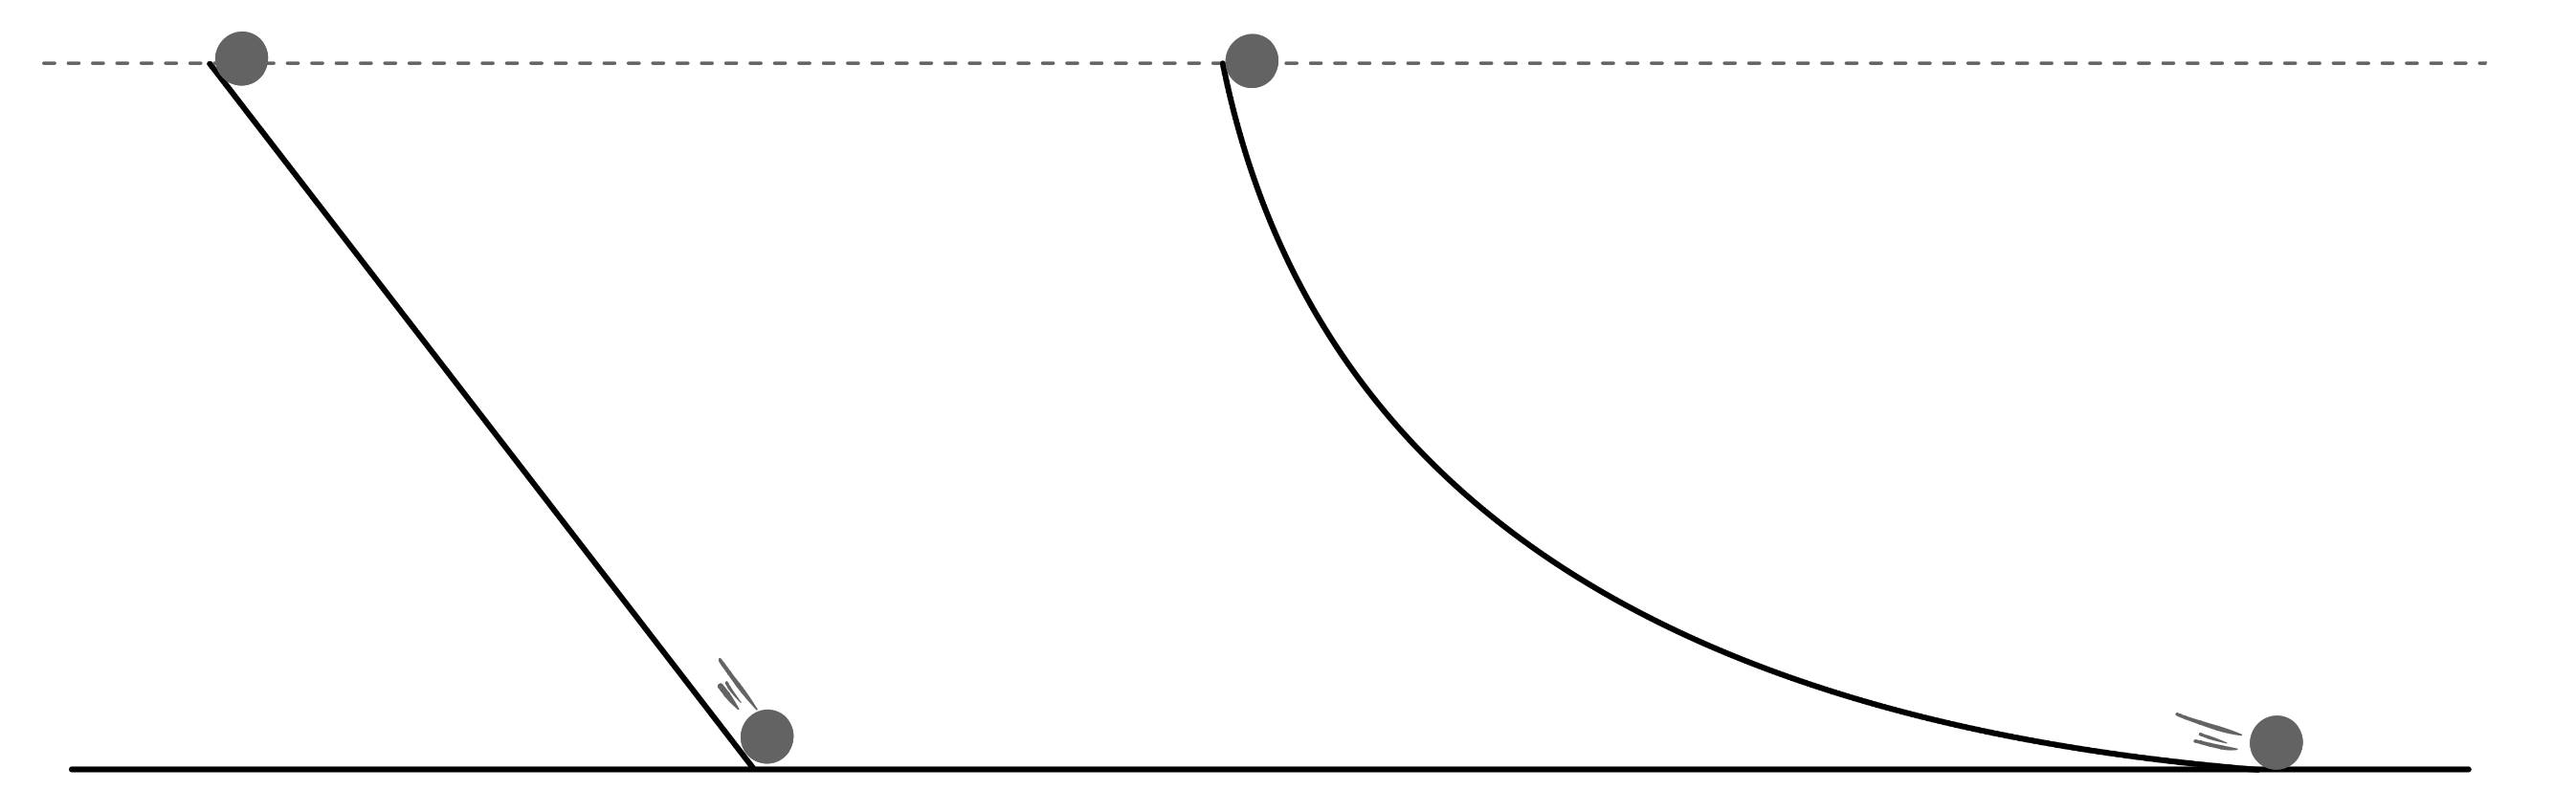
\includegraphics[width=0.9\linewidth]{imagensenergia/newtonvsleibniz1.png}
\captionof{figure}{Duas situações muito parecidas mas cujas soluções são muito diferentes.}
\label{fig_energia_newtonvsleibniz1}
} 
\vspace{0.3cm}


É claro que tal solução poderia ter sido feita -- talvez até de forma mais enxuta -- usando o conceito de conservação da energia mecânica: toda a energia cinética $\sfrac{mv^2}{2}$ adquirida pela bolinha é oriunda da perda de energia potencial $mgh$, de modo que a conservação da energia exige que 

$$ \dfrac{1}{2}mv^2 = mgh \implies \boxed{v = \sqrt{2gh},} $$

\noindent fornecendo o mesmo resultado, como esperado. Alguns poderiam alegar que a segunda solução é mais direta e mais sucinta do que a primeira, mas isso dificilmente justificaria termos feito tudo o que fizemos até aqui -- definir novas grandezas como trabalho, energia, construir dois novos teoremas (o da energia cinética e o da conservação da energia) --, para resolver um problema cuja solução já éramos capazes de construir. 

A verdadeira vantagem e a única razão de tudo o que fizemos até aqui neste capítulo é conseguir resolver um problema como o da segunda imagem da Figura \ref{fig_energia_newtonvsleibniz2}. Note que, a princípio, ele parece muito com o problema anterior: abandona-se uma bolinha, do repouso, de uma mesma altura $h$ em relação ao chão, sob a ação da mesma gravidade $g.$ A única diferença, agora, é o formato da rampa: não temos mais um plano, retilíneo, de inclinação $\theta$ constante. A nova rampa é uma curva qualquer.

\vspace{0.3cm}
{
\centering
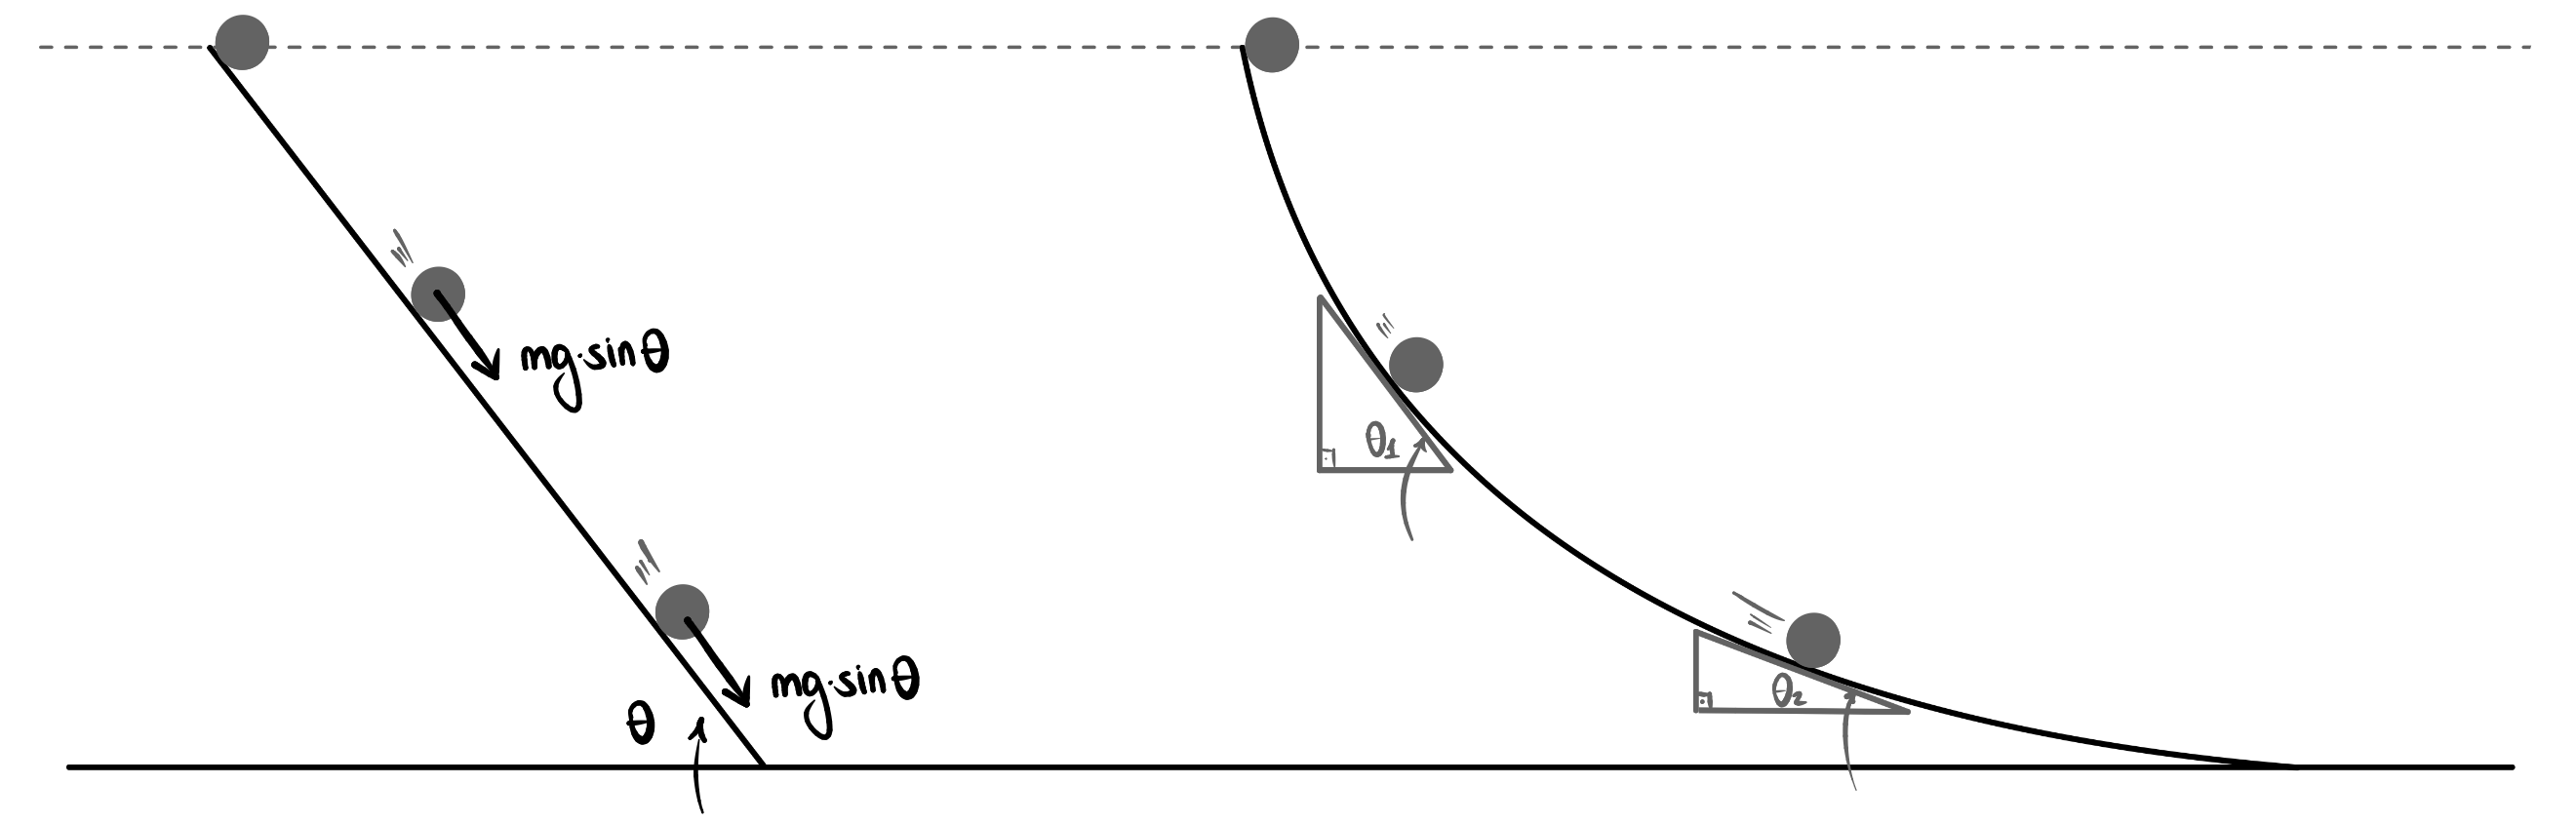
\includegraphics[width=0.9\linewidth]{imagensenergia/newtonvsleibniz2.png}
\captionof{figure}{Análise da dinâmica dos movimentos ponto a ponto.}
\label{fig_energia_newtonvsleibniz2}
} 
\vspace{0.3cm}

Neste caso, resolver pelas leis de Newton seria um trabalho de enorme complexidade operacional: poderíamos imaginar que a rampa, curva, é formado por uma sequência de vários planos inclinados de inclinações $\theta_1, \theta_2, \dots , \theta_n.$ Contudo, isso implicaria que a aceleração da bolinha seria diferente em cada estágio do seu movimento: a aceleração é mais intensa onde a inclinação da curva é mais acentuada, como em $\theta_1,$ e menos intensa aonde ela é menos acentuada, como em $\theta_2,$ representados na imagem da direita da Figura \ref{fig_energia_newtonvsleibniz2}: a bolinha acelera com mais intensidade no início da descida e com menos intensidade no final.

Dessa forma, teríamos um problema extremamente complexo: uma aceleração $g \sin \theta $ variável, haja vista que o ângulo $\theta$ varia o tempo inteiro. Não poderíamos aplicar nossas equações do MUV, uma vez que essas só se aplicam para movimentos com aceleração constante. Teríamos que construir outros tipos de equações\footnote{Isso até é possível, porém exige o uso de ferramentas matemáticas mais sofisticadas do Cálculo Integral e Diferencial.}, além de conhecer o formato geométrico exato da rampa, para saber qual é sua inclinação exata $\theta$ em cada ponto.

Note, portanto, que atacar o problema pela descrição vetorial da dinâmica -- as Leis de Newton — acarretaria complexidades justamente pelo fato de que tal raciocínio exigiria analisar ponto a ponto a dinâmica das forças que atuam na partícula, e, como visto, essas forças mudam ao longo da trajetória de um jeito nada trivial. Já a análise de trabalho e energia ignora todo o meio do caminho e exige que se tenha informações da partícula em apenas dois pontos de sua trajetória:

\begin{enumerate}
    \item [(i)] O ponto inicial, em que sua velocidade é $v_0$ e sua energia cinética, portanto, é nula. Em tal ponto a energia potencial da bola, em relação ao solo, é $E_\text{P}=mgh.$

    \item [(ii)] O ponto final, em que a energia potencial agora é nula, e toda a energia se tornou cinética.
\end{enumerate}

Com isso, a conservação da energia nos leva exatamente à mesma equação de quando resolvemos o problema para o plano inclinado:

$$ \dfrac{1}{2}mv^2 = mgh \implies \boxed{v = \sqrt{2gh}.} $$

A grande vantagem da descrição dinâmica do trabalho-energia é justamente essa: podemos olhar apenas para o início e o fim do movimento, sem nos preocuparmos com as complexas nuances que podem existir no meio do caminho. Essa é a beleza das forças conservativas: o trabalho que elas realizam independe da trajetória, de modo que é possível olhar apenas para o estado inicial e final do movimento, ignorando completamente tudo o que ocorre no meio do caminho.

Com isso, computar a velocidade final da bolinha após escorregar por qualquer uma das rampas da Figura \ref{fig_energia_newtonvsleibniz3} se torna resolver exatamente o mesmo problema -- se usarmos a teoria e os conceitos de trabalho e energia. Todas chegam no solo com exatamente a mesma velocidade: $v=\sqrt{2gh}.$ Contudo, usando as leis de Newton, os problemas são radicalmente diferentes, se tornando cada vez mais complexos, e não é possível sabermos -- por tal teoria -- que a resposta final seria a mesma em todos os casos.

\vspace{0.3cm}
{
\centering
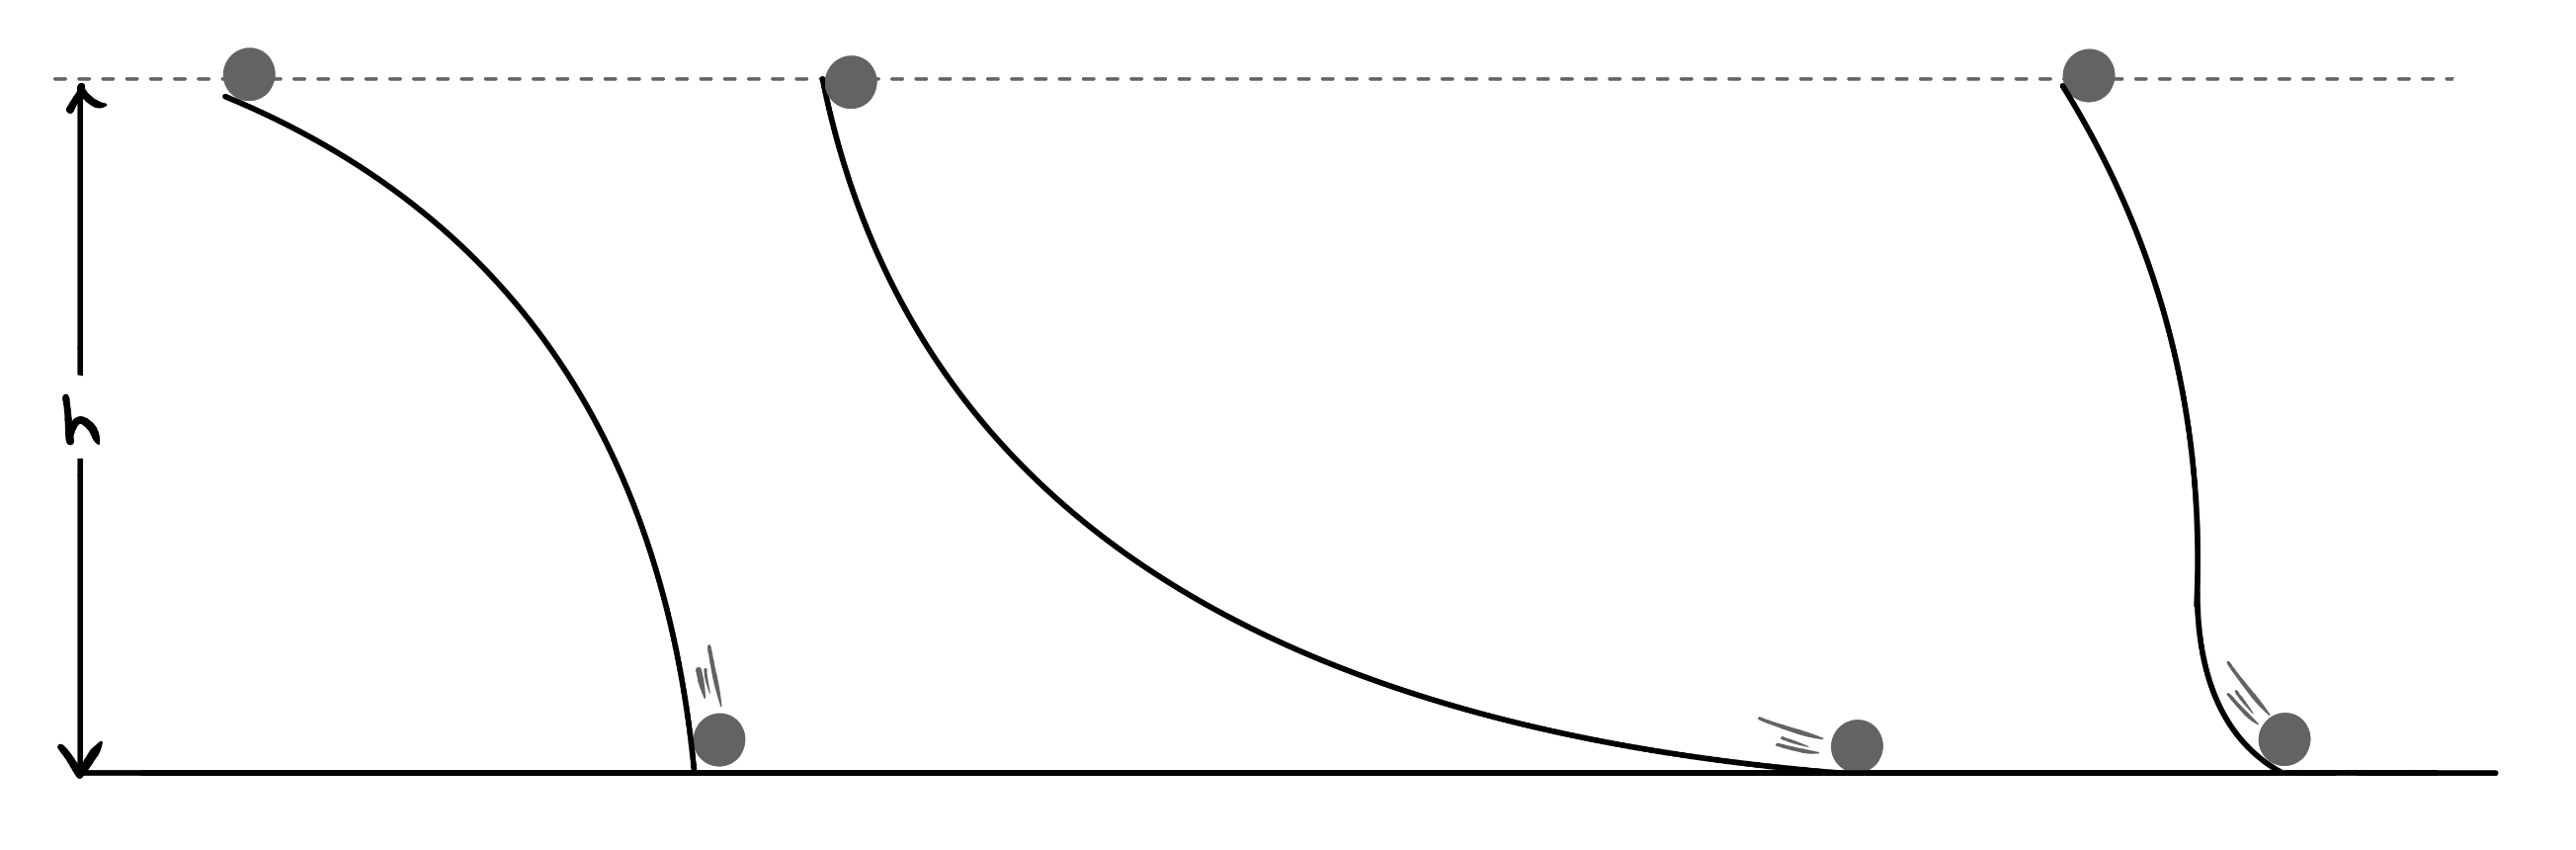
\includegraphics[width=0.9\linewidth]{imagensenergia/newtonvsleibniz3.png}
\captionof{figure}{Três problemas aparentemente distintos, mas com a mesma solução.}
\label{fig_energia_newtonvsleibniz3}
} 
\vspace{0.3cm}

Assim, espero que tal digressão tenha uma outra serventia ao leitor, além de satisfazer sua curiosidade: deixar claro em quais contextos é mais interessante se usar leis de Newton (a descrição vetorial da dinâmica) e em quais contextos é melhor usar trabalho e energia (a descrição escalar da dinâmica). Quando o meio do caminho é simples -- e o problema se reduz a um MUV -- tanto faz fazer por um método ou por outro, como é o caso da primeira situação da Figura \ref{fig_energia_newtonvsleibniz1}. Já quando o meio do caminho é complicado e incorreria em um movimento com aceleração variável -- coisa que o leitor sequer tem maturidade e matemática suficiente para encarar -- é melhor usar trabalho e energia, em que se ignora o meio do caminho.




Por fim, cabe aqui um breve contraste entre a descrição vetorial (leis de Newton) da dinâmica e a descrição escalar (trabalho e energia). Note que cada uma delas parte de uma grandeza fundamental que \emph{mede} o movimento, construindo a respectiva grandeza que gera sua \emph{variação,} o que se sintetiza em um teorema (teorema do impulso no caso newtoniano e teorema da energia cinética no caso escalar). Por fim, nas duas descrições existe uma grandeza que se conserva -- o que é o centro de cada teoria, usado para estudar a evolução dos movimentos. A tabela abaixo mostra essa relação. O leitor deve tirar algum tempo para refletir sobre ela e comparar as semelhanças fundamentais entre as duas descrições.




\begin{table}[h!]
\centering
\renewcommand{\arraystretch}{2.2}
\begin{tabular}{>{\RaggedRight\arraybackslash}p{3.2cm} | >{\centering\arraybackslash}p{3.8cm} | >{\centering\arraybackslash}p{3.8cm}}
\noalign{\hrule height 1.5pt}
\rule{0pt}{2.8ex}\textbf{Grandeza} & \textbf{Descrição Vetorial} & \textbf{Descrição Escalar} \\[0.3ex]
\noalign{\hrule height 1.5pt}
\small\textsc{que mensura o movimento}
    & $\vec{p} = m\vec{v}$
    & $E_c = \dfrac{1}{2}mv^2$ \\
\hline
\small\textsc{que mensura a variação do movimento}
    & $\vec{I} = \vec{F}\,\Delta t$
    & $W = F_{//} \cdot d$ \\
\hline
\small\textsc{relação entre as duas}
    & $\vec{I} = \Delta\vec{p}$
    & $W = \Delta E_c$ \\
\hline
\small\textsc{lei de conservação}
    & \parbox[c]{4.1cm}{\centering \rule{0pt}{2.8ex}$\Delta\vec{p} = \vec{0}$ \\[4pt]
      \small(sob a ação de\\[-2pt]forças internas)\vspace{4pt}}
    & \parbox[c]{4.1cm}{\centering \rule{0pt}{2.8ex}$\Delta E_\text{M} = 0$ \\[4pt]
      \small(sob a ação de\\[-2pt]forças conservativas)\vspace{4pt}} \\
\noalign{\hrule height 1.5pt}
\end{tabular}
\end{table}


% Note como nossas duas grandes teorias se propõem a fazer algo bem parecido: estudar como o movimento varia. Uma, contudo, usa como base grandezas vetoriais, enquanto a outra usa grandezas escalares. Os resultados, como vimos, se somam: uma teoria ilumina a sombra da outra, gerando análises que se complementam.







\vspace{0.3cm}

\begin{exemplo}[Nível I]\label{exemplo_energia_conservacaoenergiamecanica01}

Um pêndulo simples de comprimento $L = 1{,}25\ \text{m}$ é deslocado de sua posição
de equilíbrio até que o fio forme um ângulo $\theta = 60^\circ$ com a vertical, e então
solto do repouso. Qual é a velocidade do pêndulo ao passar pelo ponto mais baixo de
sua trajetória? 


\resolucao

A altura $h$ do ponto em que a massa é abandonada em relação ao ponto mais baixo é obtida pela diferença entre o comprimento do fio e sua projeção vertical:
%
\begin{equation*}
    h = L - L\cos\theta = L(1 - \cos\theta) = 1{,}25 \cdot (1 - 0{,}5)
    = 0{,}625\ \text{m}.
\end{equation*}

\vspace{0.3cm}
{
\centering
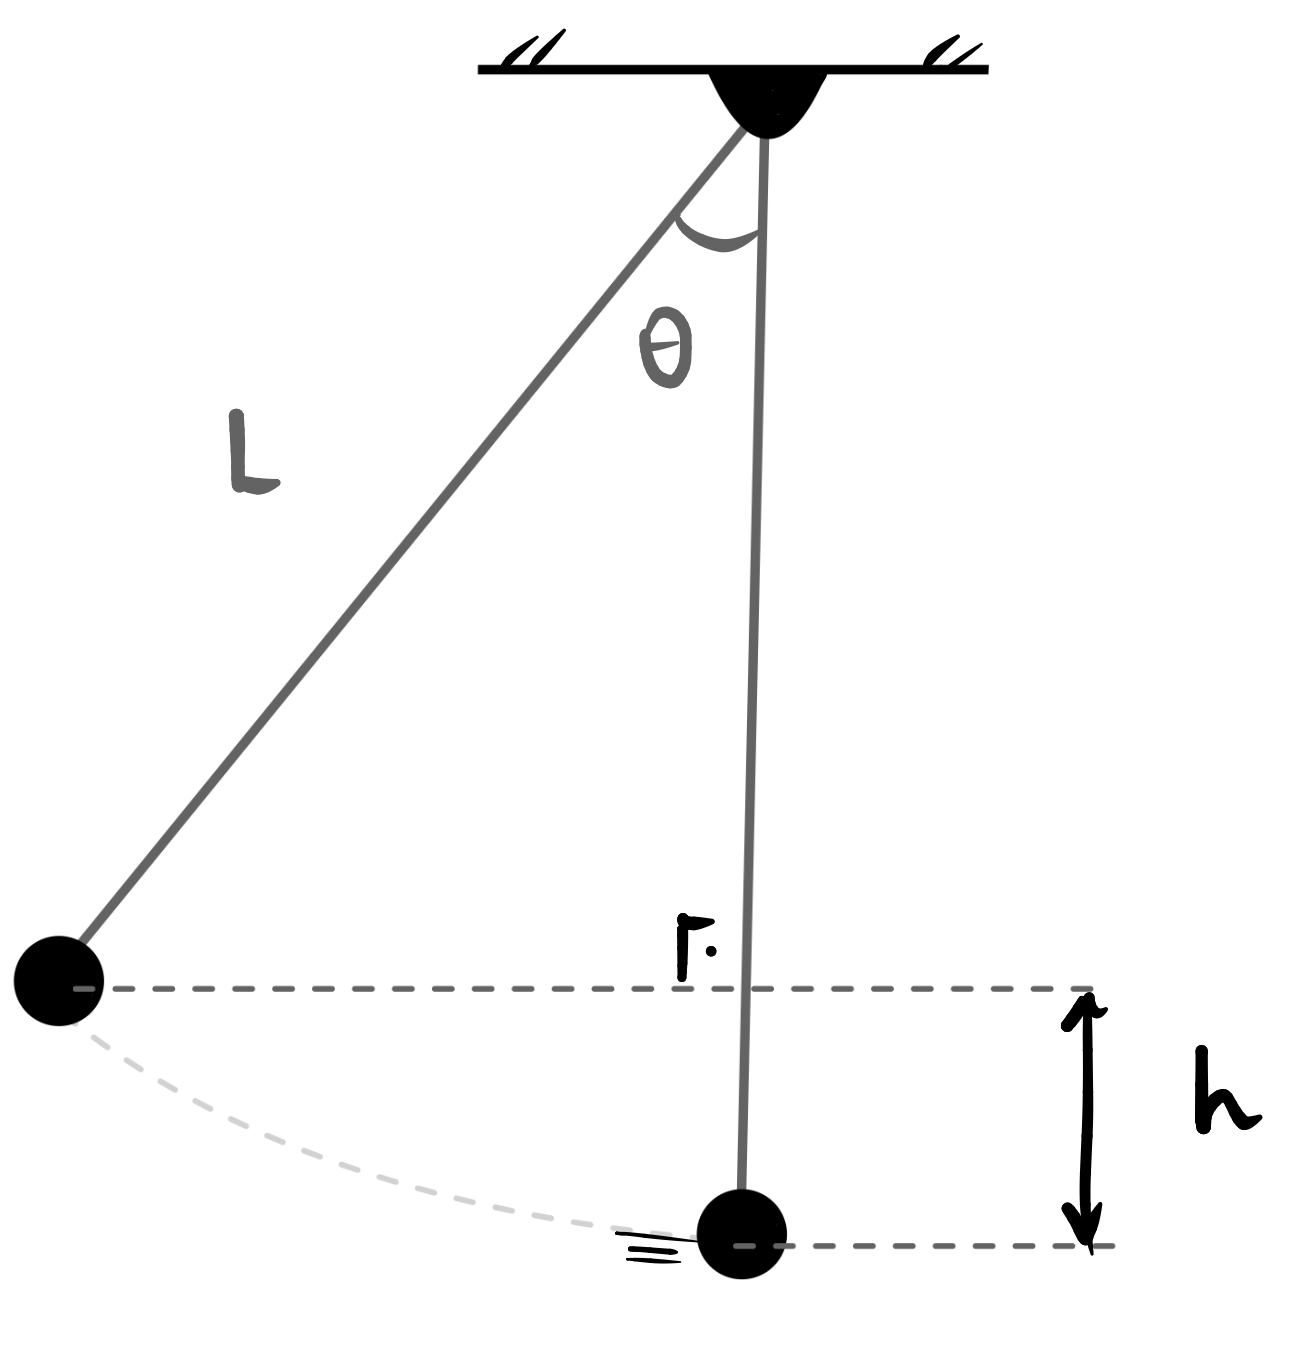
\includegraphics[width=0.30\linewidth]{imagensenergia/consenergiaex01.png}
\captionof{figure}{Conservação da energia mecânica no movimento pendular.}
\label{fig_energia_consenergiaex01}
} 
\vspace{0.3cm}

Tomando o ponto mais baixo como nível de referência e aplicando a conservação da
energia entre a posição em que a massa é abandonada (repouso, altura $h$) e o ponto mais baixo
(velocidade $v$ máxima, altura zero):
%
\begin{equation*}
    mgh = \frac{1}{2}mv^2
    \implies v = \sqrt{2gh} = \sqrt{2 \cdot 10 \cdot 0{,}625} = \sqrt{12{,}5}
    \approx 3{,}5\ \text{m/s}.
\end{equation*}

Pela Segunda Lei de Newton, esse mesmo resultado exigiria escrever as equações do
movimento circular com força resultante centrípeta variável ao longo da trajetória
curva --- um problema que, no Ensino Médio, não é tratável de forma elementar. A
conservação da energia o resolve em duas linhas, sem que seja necessário conhecer
nada sobre a trajetória entre os dois pontos.


\end{exemplo}


\vspace{0.3cm}





\begin{exemplo}[Nível II]\label{exemplo_energia_conservacaoenergiamecanica02}

Um bloco de massa $m = 2\ \text{kg}$ é solto do repouso no topo de uma rampa
circular sem atrito de raio $R = 0{,}8\ \text{m}$. No fundo da rampa, o bloco
comprime uma mola horizontal de constante $k = 2500\ \text{N/m}$ fixada a uma
parede. Determine a compressão máxima $x_0$ da mola. Adote $g = 10\ \text{m/s}^2$ e despreze os atritos.




\resolucao

Identificamos três estados relevantes: (A) bloco no topo da
rampa, em repouso, à altura $R$, mola relaxada; (B) bloco no fundo da rampa, em
movimento, à altura zero, mola ainda relaxada; (C) compressão máxima, bloco em
repouso, à altura zero, mola comprimida de $x_0$.

\vspace{0.3cm}
{
\centering
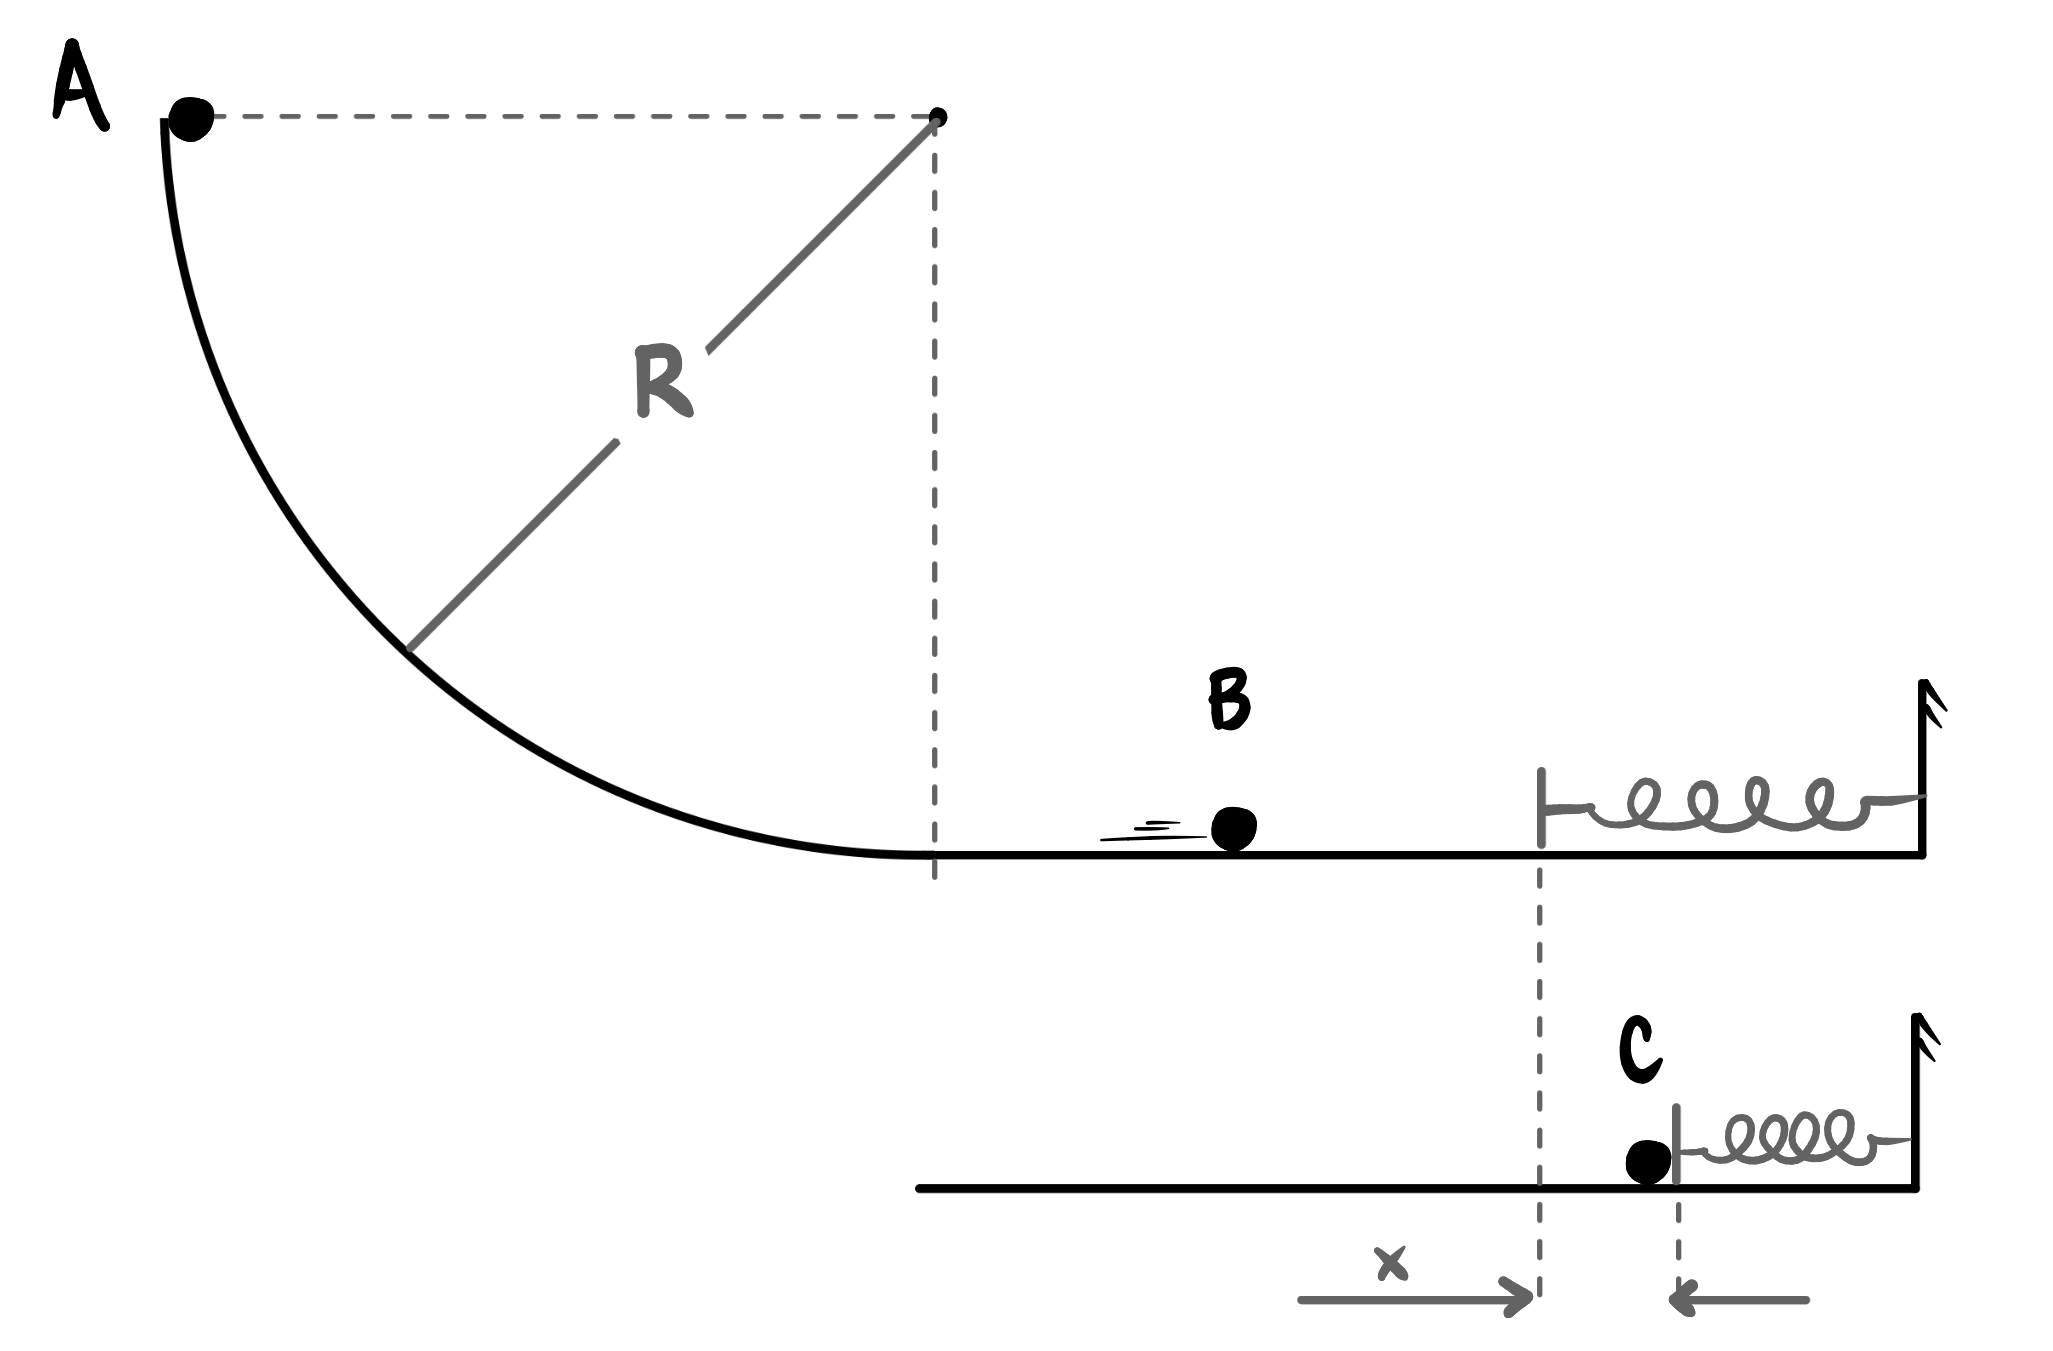
\includegraphics[width=0.5\linewidth]{imagensenergia/consenergiaex02.png}
\captionof{figure}{Conservação da energia mecânica no movimento pendular.}
\label{fig_energia_consenergiaex02}
} 
\vspace{0.3cm}

Poderíamos aplicar a conservação da energia em duas etapas (A)$\to$(B) e depois
(B)$\to$(C). Mas como a energia mecânica se conserva ao longo de \textit{todo} o
processo, podemos ir diretamente de (A) a (C), pulando o estado intermediário (B)
inteiramente, isto é: $E_{\text{M}_{A}} =E_{\text{M}_{C}},$ o que se escreve como:

\begin{align}
    E_{\text{M}_{A}} &=E_{\text{M}_{C}} \nonumber \\
     \underbrace{mgR}_{\substack{E_{PG} \text{ no topo}}} + \underbrace{0}_{E_C}
    + \underbrace{0}_{E_{PE}}
    &=
    \underbrace{0}_{E_{PG}} + \underbrace{0}_{E_C \text{ (repouso)}}
    + \underbrace{\frac{1}{2}kx_0^2}_{E_{PE} \text{ final}}. \nonumber
\end{align}

Isso resulta em

\begin{equation*}
    mgR = \frac{1}{2}kx_0^2
    \implies x_0 = \sqrt{\frac{2mgR}{k}}
    = \sqrt{\frac{2 \cdot 2 \cdot 10 \cdot 0{,}8}{2500}}
    \approx 0{,}113\ \text{m} \approx 11{,}3\ \text{cm}.
\end{equation*}

% \begin{figure}[H]
% \centering
% \begin{tikzpicture}[scale=1.0]

%     % --- Parede ---
%     \fill[pattern=north east lines] (5.0,-1.0) rectangle (5.4, 1.2);
%     \draw[thick] (5.0,-1.0) -- (5.0, 1.2);

%     % --- Mola COMPRIMIDA (mais curta) ---
%     \draw[decoration={coil, coil aspect=0.4, segment length=4pt, amplitude=4pt,
%           pre=lineto, pre length=3pt, post=lineto, post length=3pt},
%           decorate, thick] (3.85,0) -- (5.0,0);
%     % bloco encostado na mola
%     \fill[gray!50] (3.15,-0.3) rectangle (3.85, 0.3);
%     \node at (3.5, 0) {$m$};

%     % --- Chão horizontal ---
%     \draw[thick] (0,-0.3) -- (5.0,-0.3);
%     \fill[pattern=north east lines] (0,-0.6) rectangle (5.0,-0.3);

%     % --- Rampa circular ---
%     \draw[thick] plot[domain=180:270, samples=60]
%         ({-0.8*cos(\x)}, {0.5 + 0.8*sin(\x)});
%     \draw[thick] (-0.8, 0.5) -- (-0.8, 1.8);
%     \fill[pattern=north east lines] (-1.1, 0.5) rectangle (-0.8, 1.8);

%     % --- x0 comprimido ---
%     \draw[<->, >=stealth, red] (3.85, -0.65) -- (5.0, -0.65);
%     \node[below, red] at (4.42, -0.65) {$x_0$};
%     \draw[dashed, red] (3.85,-0.3) -- (3.85,-0.65);
%     \draw[dashed, red] (5.0,-0.3)  -- (5.0,-0.65);

%     % posição natural da mola (tracejada)
%     \draw[dashed, gray] (3.3,-0.3) -- (3.3, 0.5);
%     \node[above, gray] at (3.3, 0.5) {\tiny pos. natural};

%     \node[above] at (4.42, 0.2) {\small $k$};

% \end{tikzpicture}
% \caption{Estado de compressão máxima: o bloco está em repouso e toda a energia
% gravitacional inicial foi convertida em energia potencial elástica.}
% \end{figure}

A energia passou por três formas distintas ao longo do processo: gravitacional no
topo da rampa, cinética no fundo e elástica na compressão máxima. Em nenhum momento
precisamos calcular a velocidade no fundo da rampa --- ela foi um estado
intermediário que a conservação da energia nos permitiu ignorar por completo. Poderíamos ter equacionado direto a conversão de energia potencial gravitacional em elástica, isto é:

$$ mgh \to \dfrac{1}{2}kx^2 \implies mgR = \dfrac{1}{2}kx_0^2,$$

\noindent que foi justamente o resultado final que chegamos.

\end{exemplo}


\vspace{0.3cm}


\begin{exemplo}[Nível III (ITA - 2013)]\label{exemplo_energia_conservacaoenergiamecanica03}

Uma corda, de massa desprezível, tem fixada em cada uma de suas extremidades, $F$ e $G$, uma partícula de massa $m$. 
Esse sistema encontra-se em equilíbrio apoiado numa superfície cilíndrica sem atrito, de raio $r$, abrangendo um ângulo de $90^\circ$ e simetricamente disposto em relação ao ápice $P$ do cilindro, conforme mostra a figura. 
Se a corda for levemente deslocada e começa a escorregar no sentido anti-horário, o ângulo $\theta=\widehat{FOP}$ em que a partícula na extremidade $F$ perde contato com a superfície é tal que

\begin{center}
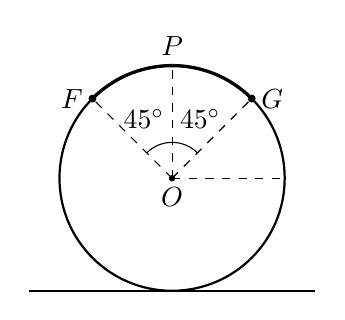
\begin{tikzpicture}[scale=0.65]
    % parâmetros
    \def\R{2.2}
    \coordinate (O) at (0,0);
    \coordinate (P) at (90:\R);
    \coordinate (F) at (135:\R);
    \coordinate (G) at (45:\R);

    % cilindro
    \draw[thick] (O) circle (\R);

    % chão
    \draw[thick] (-2.8,-\R) -- (2.8,-\R);

    % corda
    \draw[very thick] (135:\R) arc[start angle=135,end angle=45,radius=\R];

    % raios tracejados
    \draw[dashed] (O) -- (F);
    \draw[dashed] (O) -- (P);
    \draw[dashed] (O) -- (G);
    \draw[dashed] (O) -- (\R,0);

    % marcas de ângulo
    \draw (0,0.7) arc[start angle=90,end angle=135,radius=0.7];
    \draw (0,0.7) arc[start angle=90,end angle=45,radius=0.7];

    % partículas
    \fill (F) circle (2.2pt);
    \fill (G) circle (2.2pt);

    % centro
    \fill (O) circle (1.8pt);

    % rótulos
    \node[above] at (P) {$P$};
    \node[left] at (F) {$F$};
    \node[right] at (G) {$G$};
    \node[below] at (O) {$O$};
    % \node[left] at ($(F)+(-0.25,-0.2)$) {$m$};
    % \node[right] at ($(G)+(0.25,-0.2)$) {$m$};
    \node at (-0.55,1.15) {$45^\circ$};
    \node at (0.55,1.15) {$45^\circ$};
    % \node at (-1.1,-1.15) {$r$};
\end{tikzpicture}
\end{center}

\begin{enumerate}
    \item [a)] $2\cos\theta = 1$.
    \item [b)] $2\cos\theta - \sin\theta = \sqrt{2}$.
    \item [c)] $2\sin\theta + \cos\theta = \sqrt{2}$.
    \item [d)] $2\cos\theta + \sin\theta = \sqrt{2}$.
    \item [e)] $2\cos\theta + \sin\theta = \dfrac{\sqrt{2}}{2}$.
\end{enumerate}

\resolucao

\vspace{0.3cm}
{
\centering
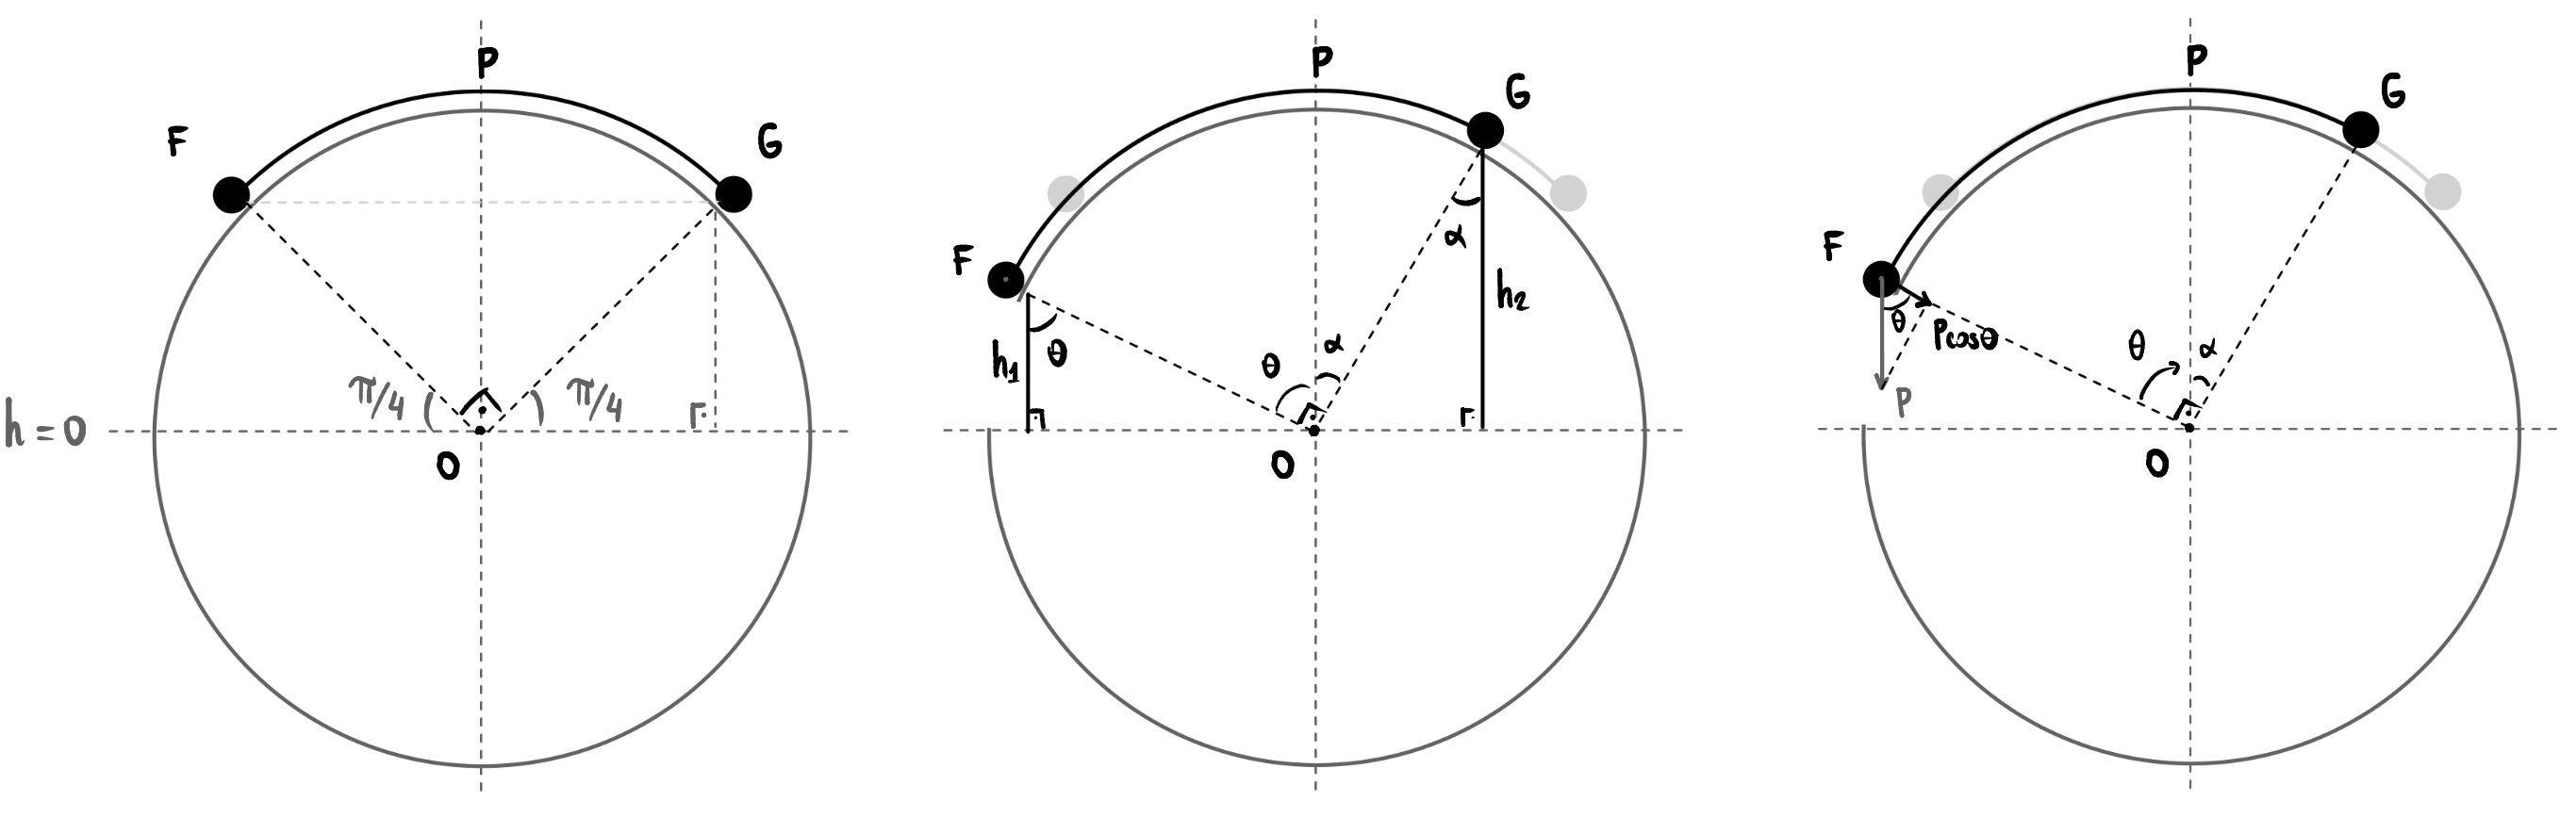
\includegraphics[width=1.0\linewidth]{imagensenergia/conservacaoenergiaitanivel3.png}
\captionof{figure}{}
\label{fig_energia_conservacaoenergiaitanivel3}
} 
\vspace{0.3cm}

A partir da primeira imagem da Figura \ref{fig_energia_conservacaoenergiaitanivel3} podemos calcular a energia mecânica inicial do sistema das duas partículas. Tomando como referência o diâmetro horizontal para o cálculo de energia potencial, a energia mecânica inicial do sistema é

$$ E_{\text{M}_i} = E_\text{P} + \cancelto{0}{E_\text{C}} = mg h_0 + mg h_0 = 2mgh_0,$$

\noindent em que $h_0$ é dado por $\sin (\sfrac{\pi}{4}) = \sfrac{\sqrt 2}{2} = \sfrac{h_0}{r},$ ou seja, $h_0 = r\sqrt 2/2,$ de modo que a energia mecânica inicial do sistema é 

\begin{equation}
     E_{\text{M}_i} = mgr \sqrt 2.
     \label{eq_consenergia_exemplo03emi}
\end{equation}

A segunda imagem da Figura \ref{fig_energia_conservacaoenergiaitanivel3} ilustra a situação em que a massa $F$ está perdendo o contato com o hemisfério. Nessa situação a energia mecânica final do sistema é


   $$ E_{\text{M}_f} = E_\text{P} + E_\text{C} = mg h_1 + mg h_2 + \dfrac{1}{2}mv^2 +  \dfrac{1}{2}mv^2,$$ 

\noindent em que $h_1=r \cos \theta$ e $h_2 = r \cos \alpha = r \cos (\sfrac{\pi}{2} - \theta) = r \sin \theta$ são facilmente obtidos pelos triângulos retângulos destacados. Note que o ângulo de abertura $\theta=F\widehat{O}P$ entre as duas partículas se mantém sempre reto: o sistema desliza como se fosse um corpo rígido. Sendo assim, o ângulo $\alpha$ é o complementar de $\theta$ e as partículas se movem sempre com a mesma velocidade $v.$ Assim, a energia mecânica final do sistema é

\begin{equation}
     E_{\text{M}_f}= mg r \cos \theta + mg r \sin \theta + mv^2.
     \label{eq_consenergia_exemplo03emf}
\end{equation}

As únicas forças que atuam nas partículas são o peso -- que é conservativo --, a normal -- que não realiza trabalho -- e a tração, porém pensando no sistema como um todo, tratam-se de forças internas que se anulam: o trabalho da tração no bloco $F$ é igual a menos o trabalho da tração no bloco $G$. Logo, somente forças conservativas realizam trabalho líquido (o peso)\footnote{Lembre-se: para aplicar o teorema de conservação da energia mecânica, em princípio, forças não-conservativas podem até atuar, o importante e imprescindível é que elas não realizem trabalho líquido.}, de modo que a conservação da energia exige que $E_{\text{M}_i}= E_{\text{M}_f},$ o que, pelas Equações \eqref{eq_consenergia_exemplo03emi} e \eqref{eq_consenergia_exemplo03emf}, se escreve como:

$$ \cancel mgr \sqrt 2 = \cancel mg r \cos \theta + \cancel mg r \sin \theta + \cancel mv^2.   $$

A terceira imagem da Figura \ref{fig_energia_conservacaoenergiaitanivel3} mostra a dinâmica das forças atuando na partícula $F$ na iminência de perder o contato: a normal (força de contato) é quase zero e apenas a componente $mg \cos \theta$ atua como resultante centrípeta:

$$ mg \cos \theta = \dfrac{mv^2}{r} \implies v^2 = rg \cos \theta, $$

\noindent o que, na relação anterior, produz

$$ gr \sqrt 2 = g r \cos \theta + g r \sin \theta + rg\cos \theta, $$

\noindent de modo que o ângulo $\theta$ deve satisfazer a equação

$$ \boxed{2 \cos \theta + \sin \theta = \sqrt 2 \implies \text{ letra D.}}$$

\end{exemplo}
\vspace{0.3cm}



% \begin{exemplo}[Nível III (ITA - 2010)]\label{exemplo_energia_conservacaoenergiamecanica03}

% Um pequeno bloco desliza sobre uma rampa e logo em seguida por um ``loop'' circular de raio $R$, onde há um rasgo de comprimento de arco $2R\varphi$, como ilustrado na figura. Sendo $g$ a aceleração da gravidade e desconsiderando qualquer atrito, obtenha a expressão para a altura inicial em que o bloco deve ser solto de forma a vencer o rasgo e continuar em contato com o restante da pista.
% \vspace{1cm}



% \begin{center}
% \begin{tikzpicture}[scale=0.6,line cap=round,line join=round]

% % parâmetros
%     %----------------------------
%     \def\R{2.0}          % raio do loop
%     \def\phi{28}         % semiabertura angular do rasgo
%     \def\th{-48}         % ponto de tangência da rampa com o círculo
%     \def\Lback{0.0}      % quanto prolongar "para trás" a rampa
%     \def\Lfwd{5.0}       % comprimento da rampa para cima

%     %----------------------------
%     % pontos principais
%     %----------------------------
%     \coordinate (O) at (0,\R);      % centro do círculo
%     \coordinate (B) at (0,0);       % ponto mais baixo do círculo

% % ponto de tangência
% \coordinate (T) at ($(O)+(\th:\R)$);

% % topo da rampa
% \coordinate (RampTop) at ($(T)+({\th+90}:8.2)$);
% \draw[thick] (T) -- (RampTop);

% % bloco sobre a rampa
% \coordinate (BlockC) at ($(T)+({\th+90}:7.2)$);
% \begin{scope}[shift={(BlockC)}, rotate={\th+90}]
%     \draw[fill=gray!20,thick] (-0.18,-0.18) rectangle (0.18,0.18);
% \end{scope}
%     % ponto de tangência da rampa no círculo
%     % \coordinate (T) at ($(O)+(\th:\R)$);

%     % % direção tangente no ponto T
%     % % raio faz angulo th; tangente faz th+90
%     % \coordinate (RampTop) at ($(T)+({\th+90}:\Lfwd)$);

%     % % posição do bloco sobre a rampa
%     % \coordinate (BlockC) at ($(T)+({\th+90}:7.0)$);

%     % base da seta da altura
%     \coordinate (Hbase) at (7.2,0);
%     \coordinate (Htop)  at ($(Hbase |- BlockC)$);

%     %----------------------------
%     % chão
%     %----------------------------
%     \draw[thick] (-3.2,0) -- (7.2,0);

%     %----------------------------
%     % loop com rasgo superior
%     %----------------------------
%     \draw[thick]
%         ($(O)+(90+\phi:\R)$)
%         arc[start angle=90+\phi,end angle=450-\phi,radius=\R];

%     % linhas tracejadas do rasgo
%     \draw[densely dashed] (O) -- ($(O)+(90+\phi:\R)$);
%     \draw[densely dashed] (O) -- ($(O)+(90:\R)$);
%     \draw[densely dashed] (O) -- ($(O)+(90-\phi:\R)$);

%     %----------------------------
%     % marcação do ângulo phi
%     %----------------------------
%     \draw[->] ($(O)+(90:0.58)$) arc[start angle=90,end angle=90+\phi,radius=0.58];
%     \node at ($(O)+(104:0.95)$) {$\varphi$};

%     %----------------------------
%     % rampa tangente ao círculo
%     %----------------------------
%     \draw[thick] (T) -- (RampTop);

%     % bloco
%     \begin{scope}[shift={(BlockC)}, rotate={\th+90}]
%         \draw[fill=gray!20,thick] (-0.18,-0.18) rectangle (0.18,0.18);
%     \end{scope}

%     %----------------------------
%     % altura h até o bloco
%     %----------------------------
%     \draw[thick,<->] (Hbase) -- (Htop);
%     \node[right] at ($(Hbase)!0.5!(Htop)$) {$h$};

%     %----------------------------
%     % rótulo R
%     %----------------------------
%     % \node at ($(O)+(-28:1.35)$) {$R$};
   
% \end{tikzpicture}
% \end{center}

% \resolucao


% \end{exemplo}
% \vspace{0.3cm}











\begin{secnivel}[Potência Mecânica]{I}{Potência Mecânica}
 

  \eqLdois{def}{eq_energia_potencia}{P := \dfrac{E}{\Delta t}}
  
\end{secnivel}







\secgfe{De onde vem}



Imagine dois operários que precisam transportar uma caixa de 50\,kg do térreo até o segundo andar de um armazém — que representa uma elevação vertical de 4\,m. Ambos chegam lá. Ambos realizaram exatamente o mesmo trabalho contra a gravidade:

\[
W = mgh = 50 \cdot 10 \cdot 4 = 2000\ \text{J}
\]

O trabalho é idêntico. A energia transferida é idêntica. E, no entanto, o primeiro operário levou 8 segundos e o segundo levou 2 minutos, ofegante e parando a cada degrau.

O leitor sente que há algo diferente nessas duas situações — algo que as grandezas \textit{trabalho} ou \textit{energia} não capturam. O primeiro operário tem um ritmo de transferência de energia muito maior que o segundo. Mas como podemos medir isso?

Note que é exatamente para isso que definimos na Equação \eqref{eq_energia_potencia}: a taxa à qual a energia é transferida ou transformada. Essa equação não descreve uma lei da natureza nem é derivada de outras grandezas -- ela dá nome a algo que a física precisava nomear: a rapidez com que a energia é transferida ou transformada. 

Potência não é o quanto de energia foi transferido. Potência é o \textit{quanto, por segundo}. A Equação \eqref{eq_energia_potencia} vem de uma necessidade semelhante àquela que tínhamos quando definimos a Equação \eqref{mecanica_eq_velocidademedia}: de medir o quão rápido algum processo ocorre.

Lá, o processo em questão era o movimento de um corpo. Aqui, é o processo de transferência de energia. Perceba, portanto, que a \eqref{eq_energia_potencia} mede justamente a \emph{velocidade} com que uma certa quantidade de energia $E$ é transferida em um processo que leva um intervalo de tempo $\Delta t$ para ocorrer.

A unidade no SI de potência é, em homenagem à James Watt -- cuja história em breve conheceremos -- o Watt (W). Ou seja:

$$ 1 \text{ W} =  \dfrac{1 \text{ J}}{\text{ s}}.$$

% O leitor poderia perguntar: por que dividimos energia pelo tempo? Por que não multiplicamos, ou elevamos ao quadrado? A resposta é a mesma de sempre nas definições: porque essa é a combinação que \textit{funciona} -- a que descreve o que queremos descrever de forma linear e intuitiva. Se dobrarmos a energia transferida no mesmo tempo, a potência dobra. Se transferirmos a mesma energia em metade do tempo, a potência dobra. Esse comportamento é exatamente a razão $E/\Delta t$ -- não $E^2/\Delta t$ ou $\sqrt{E/\Delta t}$.

% Existe também uma coerência estrutural com outras definições que o leitor já conhece. Velocidade média foi definida como $\Delta s / \Delta t$ -- deslocamento por tempo. Aceleração média, $\Delta v / \Delta t$ -- variação de velocidade por tempo. Potência segue o mesmo padrão: $E / \Delta t$ — energia por tempo. Há uma gramática na física, e potência fala a mesma língua.


\secgfe{Onde é usada}

O conceito de potência é usado em praticamente qualquer contexto no qual haja interesse em se medir o quão rápido a energia é consumida/transferida para um corpo.

Ao ligar a luz da sua casa, você tem o interesse em saber quanto de energia você consumirá (e, portanto, quanto irá gastar) para cada minuto ou hora que a lâmpada fica ligada. Por isso, ao comprar uma lâmpada, virá informado em sua caixa qual é a sua potência: 24W, 36W ou qualquer que seja o valor.

O seu chuveiro também vem com essa informação: 5.500W de potência máxima. Isso quer dizer que ele consumirá 5.500 joules de energia elétrica para cada segundo que estiver ligado. Aparelhos de ar condicionado, geladeiras, fogão e praticamente qualquer outro dispositivo elétrico terá uma potência associada a ele. Quanto maior for essa potência, mais energia tal dispositivo consumirá por unidade de tempo -- e mais caro será a sua conta de luz.

Diversas equações da física envolvem, portanto, a potência. Desde a termodinâmica, para o cálculo de potência de máquinas térmicas, como motores, ou de refrigeradores, como uma geladeira; até à elétrica, no cálculo de potências em resistores e dispositivos elétricos como uma lâmpada, um chuveiro ou uma televisão.

\secgfe{Erros comuns}

O erro mais comum é acabar confundindo potência com energia. Isso acontece, talvez, por um uso equivocado desses termos no cotidiano, em que é comum dizerem que uma lâmpada ``tem 60 watts de energia'' ou que um carro ``tem muita energia''. Ambas as frases estão erradas.

Uma lâmpada de 60\,W transfere 60 joules de energia por segundo. Ela não ``tem'' 60\,J —
ela gasta 60\,J a cada segundo que permanece acesa. Energia é o que foi transferido;
potência é o ritmo de transferência.




O kWh, por exemplo, gera uma confusão comum. O  quilowatt-hora (kWh) é uma unidade de energia -- aquela que mede o seu consumo energético na conta de luz -- não de potência:

\[
1\ \text{kWh} = 1000\ \text{W} \cdot 3600\ \text{s} = 3{,}6 \cdot 10^{6}\ \text{J} = 3{,}6\ \text{MJ}
\]

O kWh, portanto, é simplesmente uma unidade de energia conveniente para escalas domésticas. Dizer ``gastei 150\,kWh esse mês'' é o mesmo que dizer ``foram transferidos $150 \cdot 3{,}6$\,MJ de energia elétrica para o interior da minha casa nesse mês.'' A potência da sua residência
em determinado instante seria kWh dividido pelas horas -- ou seja, kW.

Portanto, lembre-se: potência se mede em watts (W); energia se mede em joules (J) ou kWh.
Se o problema pede quanto um aparelho vai gastar em 2 horas, a resposta é uma energia --
não uma potência. Se pede com qual rapidez ele transfere energia, é uma potência\footnote{O leitor pode pegar a conta de luz da sua casa e verificar que o que se paga mensalmente é justamente os kWh -- a energia consumida.}.



\secgfe{Observações}

No final do século XVIII, o engenheiro escocês James Watt tinha um problema. Ele havia aprimorado radicalmente a máquina a vapor -- tornando-a mais eficiente, mais confiável, mais econômica em combustível. Mas seus potenciais compradores, os donos de minas de carvão e fábricas têxteis do norte da Inglaterra, não entendiam de física. Eles entendiam de cavalos.

Os cavalos eram a principal tecnologia de tração da época. Cada mineradora sabia exatamente quantos cavalos precisava para bombear água de suas minas, içar carvão, mover moinhos. A pergunta natural que faziam a Watt era sempre a mesma: \textit{``quantos cavalos a sua máquina substitui?''}

Era uma pergunta de potência -- embora ninguém usasse essa palavra ainda. Um cavalo é eficiente em uma tarefa quando consegue puxar um carrinho cheio de carvão, da mina até um galpão, em, digamos, 120 segundos. Se ele fizer a mesma tarefa -- o mesmo gasto energético -- em 30 minutos, seria completamente ineficiente. Perceba, portanto, que ao comparar o desempenho de uma máquina a vapor com um cavalo, o que procuramos saber é quanto de energia, por unidade de tempo, essa máquina consegue entregar. 

\vspace{0.3cm}
{
\centering
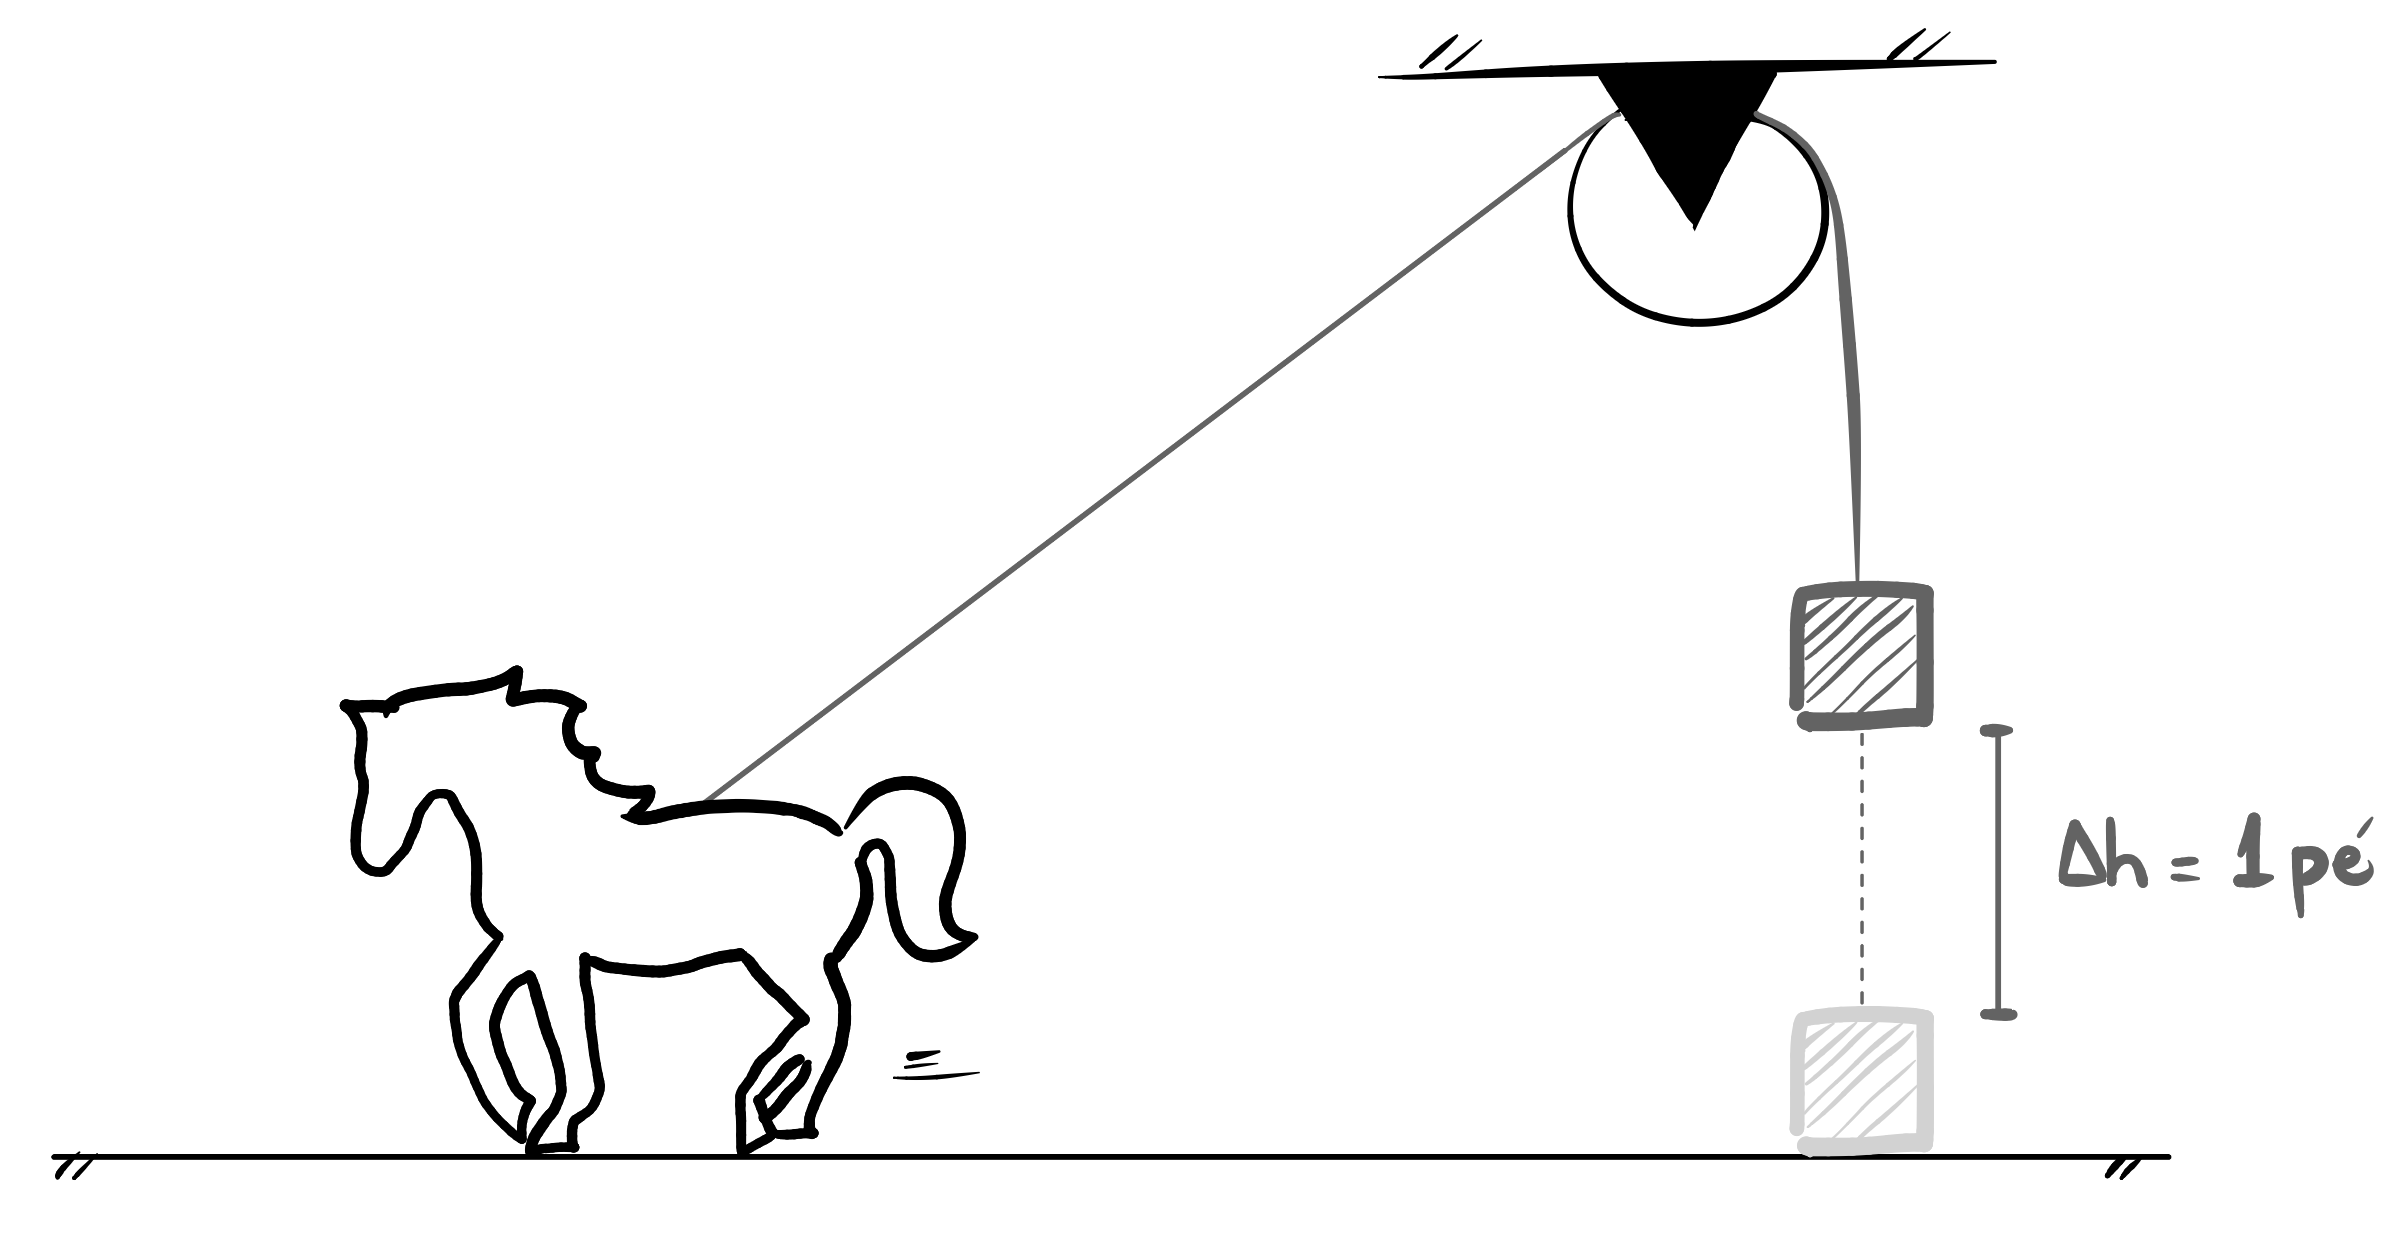
\includegraphics[width=0.5\linewidth]{imagensenergia/cavalovapor.png}
\captionof{figure}{O cálculo da potência de um cavalo: o \emph{cavalo-vapor.}}
\label{fig_energia_cavalovapor}
} 
\vspace{0.3cm}


Para responder essa pergunta, Watt precisava \textit{medir} a potência de um cavalo. O relato mais difundido é que ele realizou experimentos com cavalos de mina e observou que um cavalo típico conseguia elevar um peso de 550 libras a uma altura de 1 pé em 1 segundo, de forma sustentada. Convertendo para o SI, 1 pé $ \approx 0.3048$m; $550$lb $\approx 249.5$kg; de modo que a potência de 1 cavalo seria de

$$ P = \dfrac{E}{\Delta t} = \dfrac{W}{\Delta t} = \dfrac{F \cdot d}{\Delta t} =  \dfrac{2.445,1 \text{N} \cdot 0.3048 \text{m}}{1 \text{ s}} \approx \dfrac{746\text{ J}}{\text{s}} = \boxed{746 \text{ W} = 1 \text{ HP.}} $$



A unidade HP é o \emph{cavalo-vapor} (\emph{horse-power}), e uma potência de 1 cavalo vapor é exatamente igual à potência de um cavalo: ele entrega 746J de trabalho em 1 segundo.

Com esse número em mãos, Watt podia finalmente responder: \textit{``minha máquina Modelo~A equivale a 20 cavalos.''} O comprador entendia imediatamente o que estava comprando.

Um outro conceito que pode ser útil é o de \emph{rendimento,} representado pela letra $\eta$, e definido como a razão entre a potência útil e a potência total de uma máquina:

$$ \boxed{\eta = \dfrac{P_\text{ÚTIL}}{P_\text{TOTAL}}.}$$

O cálculo do rendimento está associado justamente ao fato de que, em qualquer processo, sempre há perdas. Assim, se um cavalo consegue imprimir uma potência, digamos, de $1000$ W, ao transferir essa energia -- por cordas, polias e sistemas desse tipo -- um pouco de energia sempre se perde no meio do caminho, de modo que a \emph{potência útil} final, ou seja, a potência que realmente é utilizada para realizar algum trabalho, é sempre menor do que isso. Digamos que ela seja de 900 W, de modo que, neste caso, o rendimento é de

$$ \eta = \dfrac{900\text{ W}}{1000 \text{ W}} = 90 \%.$$

Perceba que o rendimento se trata de um número adimensional. Note que uma máquina ter um rendimento maior do que a outra não necessariamente significa que ela seja melhor. Imagine uma máquina $A$ com potência total de 100 W e rendimento de 80\%, e uma outra máquina $B$, com potência total de $500 $ W e rendimento de 60\%. A máquina $A$ consegue entregar uma potência útil de 

$$ P_\text{A} = \eta \cdot P_\text{TOTAL} = 0.8 \cdot 100 = 80 \text{ W,}$$

\noindent enquanto a máquina $B$ entrega uma potência útil de

$$ P_\text{B} = \eta \cdot P_\text{TOTAL} = 0.6 \cdot 500 = 300 \text{ W.}$$

Se você precisa realizar uma tarefa que consuma 300 joules de energia por segundo, a máquina $B$ será a ideal entre as duas, ainda que ela \emph{desperdice} mais energia do que a máquina $A$: no final do dia ela consegue entregar uma potência útil maior.


\vspace{0.3cm}

\begin{exemplo}[Nível I]\label{exemplo_energia_potenciaex01}

Um elevador eleva uma carga de 300\,kg a uma altura de 10\,m em 15\,s,
em movimento uniforme. Qual é a potência desenvolvida pelo motor?
Adote $g = 10\ \text{m/s}^2$.

\resolucao

Em movimento uniforme, a força do motor iguala o peso da carga:
\[
F = P = mg = 300 \cdot 10 = 3000\ \text{N}
\]
O trabalho realizado pelo motor contra a gravidade:
\[
W = F \cdot d = 3000 \cdot 10 = 30\,000\ \text{J}
\]
A potência média é, portanto:
\[
P = \frac{W}{\Delta t} = \frac{30\,000}{15} = 2000\ \text{W} = 2\ \text{kW}.
\]

\medskip
\noindent Vale notar: 2\,kW é menos de 3\,CV. Um motor de motocicleta -- das mais simples --
tem mais potência que esse elevador. Isso ocorre por escolha: elevadores comerciais
são lentos por segurança e economia, não por falta de motor disponível.

\end{exemplo}


\vspace{0.3cm}





\begin{exemplo}[Nível II]\label{exemplo_energia_potenciaex02}

Considere um elevador, com 600 kg de massa e 5 passageiros, de 80 kg cada, subindo com velocidade constante.

\begin{enumerate}
    \item [a)] Mostre que a potência mecânica exercida pelo motor do elevador pode ser computada por $P=F\cdot v,$ em que $v$ é a velocidade do elevador e $F$ e força de tração nos cabos gerada pelo motor.

    \item [b)] Se o elevador sobe $12$m em 10 segundos, calcule a potência útil do motor.

    \item [c)] Sendo o rendimento do motor de 60\%, calcule sua potência real.
\end{enumerate}



\resolucao



\noindent\textit{a)} Em movimento uniforme, a força de tração $F$ nos cabos
equilibra o peso total do sistema. O trabalho realizado pelo motor ao longo
de um deslocamento $d$ é:
\[
    W = F \cdot d
\]
Dividindo ambos os lados pelo intervalo de tempo $\Delta t$ necessário para
percorrer $d$:
\[
    \frac{W}{\Delta t} = F \cdot \frac{d}{\Delta t}
\]
O lado esquerdo é, por definição, a potência média $P$. O lado direito contém
$d/\Delta t$, que é a velocidade $v$ do elevador. Portanto:
\[
    \boxed{P = F \cdot v.}
\]

\medskip
\noindent\textit{b)} A massa total do sistema é:
\[
    m = 600 + 5 \cdot 80 = 600 + 400 = 1000\ \text{kg}
\]
Em velocidade constante, a força de tração iguala o peso total:
\[
    F = mg = 1000 \cdot 10 = 10\,000\ \text{N}
\]
A velocidade de subida é:
\[
    v = \frac{d}{\Delta t} = \frac{12}{10} = 1.2\ \text{m/s}
\]
Portanto, a potência útil do motor é:
\[
    P_{\text{útil}} = F \cdot v = 10\,000 \cdot 1.2 = 12\,000\ \text{W}
    = 12\ \text{kW}.
\]

\medskip
\noindent\textit{c)} O rendimento $\eta$ relaciona a potência útil à potência real
(total fornecida pelo motor):
\[
    \eta = \frac{P_{\text{útil}}}{P_{\text{real}}}
    \implies
    P_{\text{real}} = \frac{P_{\text{útil}}}{\eta}
    = \frac{12 \text{ kW}}{0{,}60}
   = 20 \text{ kW}.
\]
Os outros 40\% da potência real — 8\,kW — são dissipados como
calor no motor, no sistema de cabos e nos mecanismos de transmissão.



\end{exemplo}
\vspace{0.3cm}





\begin{exemplo}[Nível III]\label{exemplo_energia_potenciaex03}
Uma pedra de massa $m$ é largada do repouso a uma altura $H$ acima do solo.
Considere apenas a força gravitacional ($g$ constante, sem resistência do ar).

\begin{enumerate}
    \item [a)] Determine a potência instantânea desenvolvida pela gravidade em
    função do tempo $t$.

    \item [b)] Determine a potência média da gravidade ao longo de toda a queda.

   
\end{enumerate}

\resolucao

\noindent\textit{a)} A força gravitacional é $F = mg$ (constante, dirigida para baixo).
A velocidade do objeto no instante $t$, partindo do repouso, é $v(t) = gt$.
Aplicando $P = Fv$:
\[
    P_{\text{inst}}(t) = mg \cdot gt = mg^2 t
\]
A potência instantânea da gravidade cresce \textit{linearmente} com o tempo:
ela é nula no instante inicial (objeto em repouso) e aumenta continuamente
durante toda a queda.

\medskip
\noindent\textit{b)} O trabalho total realizado pela gravidade ao longo da queda de
altura $H$ é:
\[
    W = mgH
\]
O tempo de queda $t_f$ é obtido de $H = \dfrac{1}{2}g t_f^2$:
\[
    t_f = \sqrt{\frac{2H}{g}}
\]
A potência média é, então:
\[
    \bar{P}
    = \frac{W}{t_f}
    = \frac{mgH}{\sqrt{2H/g}}
    = \frac{mgH\sqrt{g}}{\sqrt{2H}}
    = mg\sqrt{\frac{gH}{2}}
\]


\end{exemplo}
